% options:
% thesis=B bachelor's thesis
% thesis=M master's thesis
% czech thesis in Czech language
% english thesis in English language
% hidelinks remove colour boxes around hyperlinks

\documentclass[thesis=M,english]{FITthesis}[2012/10/20]

\usepackage[utf8]{inputenc} % LaTeX source encoded as UTF-8
% \usepackage[latin2]{inputenc} % LaTeX source encoded as ISO-8859-2
% \usepackage[cp1250]{inputenc} % LaTeX source encoded as Windows-1250

\usepackage{graphicx} %graphics files inclusion
% \usepackage{subfig} %subfigures
% \usepackage{amsmath} %advanced maths
% \usepackage{amssymb} %additional math symbols

\usepackage{dirtree} %directory tree visualisation

\usepackage{listings}
% % list of acronyms
% \usepackage[acronym,nonumberlist,toc,numberedsection=autolabel]{glossaries}
% \iflanguage{czech}{\renewcommand*{\acronymname}{Seznam pou{\v z}it{\' y}ch zkratek}}{}
% \makeglossaries

\usepackage{color}
\definecolor{lightgray}{rgb}{.9,.9,.9}
\definecolor{darkgray}{rgb}{.4,.4,.4}
\definecolor{purple}{rgb}{0.65, 0.12, 0.82}
\lstdefinelanguage{JavaScript}{
  keywords={break, case, catch, continue, debugger, default, delete, do, else, false, finally, for, function, if, in, instanceof, new, null, return, switch, this, throw, true, try, typeof, var, void, while, with},
  morecomment=[l]{//},
  morecomment=[s]{/*}{*/},
  morestring=[b]',
  morestring=[b]",
  ndkeywords={class, export, boolean, throw, implements, import, this},
  keywordstyle=\color{blue}\bfseries,
  ndkeywordstyle=\color{darkgray}\bfseries,
  identifierstyle=\color{black},
  commentstyle=\color{purple}\ttfamily,
  stringstyle=\color{red}\ttfamily,
  sensitive=true
}

\lstset{
   language=JavaScript,
   backgroundcolor=\color{lightgray},
   extendedchars=true,
   basicstyle=\footnotesize\ttfamily,
   showstringspaces=false,
   showspaces=false,
   numbers=left,
   numberstyle=\footnotesize,
   numbersep=9pt,
   tabsize=2,
   breaklines=true,
   showtabs=false,
   captionpos=b
}

% % % % % % % % % % % % % % % % % % % % % % % % % % % % % % 
% EDIT THIS
% % % % % % % % % % % % % % % % % % % % % % % % % % % % % % 

\department{Department of Software Engineering}
\title{GPS pinned messaging application}
\authorGN{Daria} %author's given name/names
\authorFN{Mikhailova} %author's surname
\author{Mikhailova Daria} %author's name without academic degrees
\authorWithDegrees{Mikhailova Daria \& Bc.} %author's name with academic degrees
\supervisor{Ing. Jan Vaclavik}
\acknowledgements{I would like to thank my supervisor Ing. Jan Vaclavik for his assistance and advice while leading this project and for giving me a chance to learn new technologies and bring one of my ideas to life.}
\abstractEN{The goal of this thesis is to explore a new way of creating mobile applications using Javascript technologies and implement a complete system for messaging. The system will comprise of mobile application in React Native which brings a new way of communicating by leaving messages at GPS locations, web application in React and a REST API server in node.js.}
\abstractCS{V n{\v e}kolika v{\v e}t{\' a}ch shr{\v n}te obsah a p{\v r}{\' i}nos t{\' e}to pr{\' a}ce v {\v c}esk{\' e}m jazyce.}
\placeForDeclarationOfAuthenticity{Prague}
\keywordsCS{Replace with comma-separated list of keywords in Czech.}
\keywordsEN{GPS messaging, React Native, React, Node.js, Redux, Augmented Reality, Wikitude.}
\declarationOfAuthenticityOption{1} %select as appropriate, according to the desired license (integer 1-6)


\begin{document}

% \newacronym{CVUT}{{\v C}VUT}{{\v C}esk{\' e} vysok{\' e} u{\v c}en{\' i} technick{\' e} v Praze}
% \newacronym{FIT}{FIT}{Fakulta informa{\v c}n{\' i}ch technologi{\' i}}

\setsecnumdepth{part}
\chapter{Introduction}

The rapid usage growth of messaging apps over the past several years can only be described as astronomic. Currently mobile messaging applications are offering so much more than just simple messaging and media exchange. Some of them connect users with brands, bring news and even let you shop through them. Messaging apps's user base is outweighing the most popular social networks.\cite{BI-apps} As you can see on figure \ref{fig:apps}, which compares WhatsApp, Facebook Messenger, WeChat and Viber to Facebook, Linkedin, Twitter and Instagram. The scale is in billions of users.\cite{hubspot}


\begin{figure}[!ht]
	\centering
	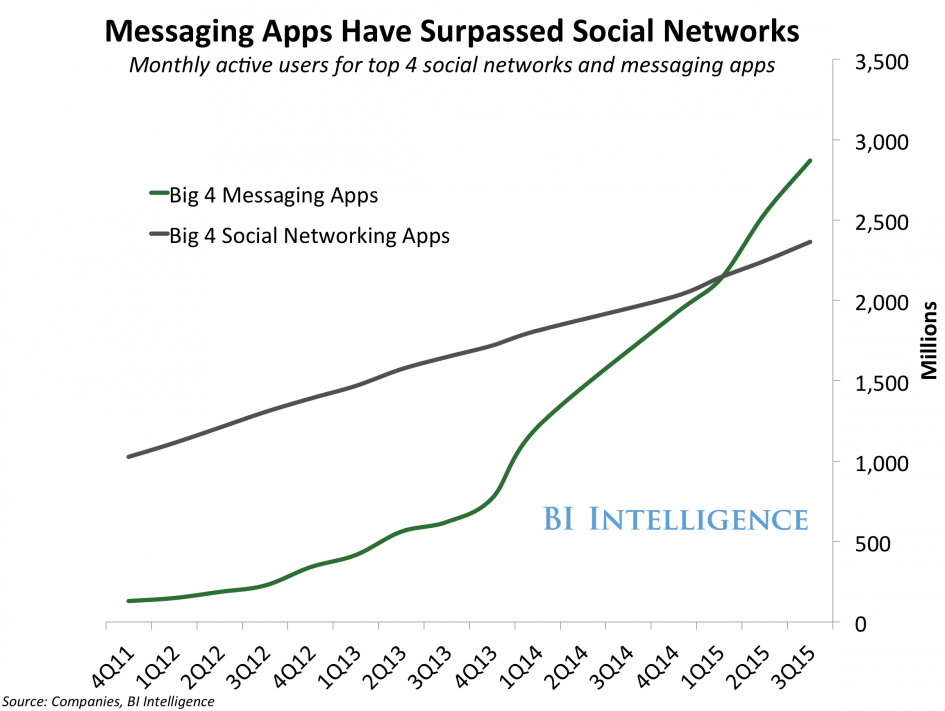
\includegraphics[width=0.9\textwidth]{assets/messaging_apps.png}}
	\caption{Messaging apps have surpassed social networks \\ Source: \cite{BI-apps}	}
	\label{fig:apps}
\end{figure}

All of the mentioned above makes messaging applications and social networks a vital part of our life. Nevertheless the rapid growth in functionality let's not forget their main aim. The main aim of both types is to connect people and  let them exchange messages in a cheap and easy way. Both messaging application and social network fulfil this goal very well. However there is a certain communication gap which has not been addressed yet.

We use messaging applications and social media to communicate with people we already know. We become highly suspicious when it comes to meeting new people in the case we do not have any friends in common. Let's use Facebook as an example. To be honest Facebook was not created for connecting with strangers and its main purpose is to stay connected with your friends and family. The old superstition that many people online, who are not your acquaintances, are not who they pretend to be is still on. So how do we meet new people online? Facebook offers many interest clubs and event pages where we come in contact with people we do not know, but hardly any meetings or friendships arise from that. Internet also offers old school forums and communities where people talk about their common interests such as movies or music. But in case you just want to meet someone not based on your interest, just a random person the only way to do it is via a dating site. You have to sign up for a dating website or download an app such as Tinder. There are many people on dating sites who are just looking for friends and not long life partners. In the wide circles looking for friends on dating websites is considered slightly strange. If you are extravert enough you can just meet people on the street or in the bus. But what do you do when you are in a foreign country? What do you do when you are just wandering around looking for a company to do some sightseeing? What if you just really liked this museum and want to find so-thinking people without the whole going extremely public about it?

Meet the GPS pinned messaging application. The idea is very simple. Usual messaging applications require the communicating parties to identify themselves with each other, either using their phone numbers or emails. This creates a certain barrier in communication. People are not that interested or afraid of just chatting with strangers online since in order to do so they have to reveal a lot of their personal information to the other party. The GPS pinned messaging application does not require any details from the other party in order to communicate. Imagine you are travelling and you just moved in a hotel. You do not know anyone in the city and would like to have a company for the sightseeing. In this case you just leave a message right on the GPS location of your room and everyone in the hotel would see it, since they would be within a shorsert reach o your GPS location. Anyone could answer your message and probably very quickly you will manage to find yourself a company for the walk in the city.

GPS messaging application allows a user to leave messages pinned to GPS location anywhere. It could be a review message saying how much someone liked a certain gallery or a message warning fellow travellers of scams or robberies happening in the area. University students could exchange messages with the whole lecture hall during the lecture. The only way to read such a message is to be within short distance of it. You cannot read the message if you are far away. This makes messaging a quest, when you go through the city with new messages appearing on the map. This brings freedom in messaging. It is almost the same as you would go and directly talk to someone. This messaging style leaves out all the unnecessary information which you have on the social networks, it keeps the users identity private and therefore you do not know complete biography of a person before talking to them. And most importantly it allows you to interact with anyone who is within your GPS reach. It is private and public at the same time, limited by location and messages validity only.

\setsecnumdepth{all}
\chapter{Requirements}

The main goal is to create a system consisting of a messaging application which will allow users to pin messages to GPS location, web application for uploading 3d objects and viewing statistics and a REST API server to communicate with both of them. 

Messaging application will offer two types of messages. Firstly users will post simple text messages with an option of attaching a picture. Secondly users will be able to post a 3D object. Both types of messages are comment-able. Each posted message can have a validity from 1 day up to 365 days. Users are only able to read a message once they arrive at its GPS location. The user will be able to browse through his messages and in case someone commented on his message he will be notified of it. 

Web application is a complimentary portal which allows to browse through a common 3d gallery and choose objects for messages, upload your own 3d objects and view messaging statistics.

The server will be providing data for both applications and will also serve as an authorization authority.

\section{System functional requirements}

\begin{enumerate}
\item{Registration}

User can register using their email and password using mobile application.

\item{Authentication}

Users will be authenticated through tokens using OAuth 2 protocol. 

\item{Leave a message}

The user is able to leave a message pinned to his/her GPS location using mobile application. There is an option of adding an image to the message.

\item{Leaving a 3D object}

The user is able to leave a 3D object pinned to his/her GPS location. The user can choose a 3D object from the gallery of objects or upload their own object following the instructions on the web.

\item{Read a message}

The user is able to read a message only once he/she is close to its GPS location.

\item{Comment message}

The user is able to comment any message he stumbled upon.

\item{User browses through his messages}

The user will be able to browse through a list of the messages he posted and see how many people viewed the message and whether there are any new comments since the last time he viewed the message.

\item{View statistics}

Users can view statistics of their messages, for instance how many times the message has been viewed and how many comments were left. There will also be general statistics for everyone showing popularity of different countries by the number of messages.

\item{View and change user details}

The user will be able to update his profile using mobile application. He will be able to upload a profile picture, choose a country, change email or password.

\end{enumerate}


\subsection{System non functional requirements}

\begin{enumerate}

\item{Performance} 

There must be short response time for server requests. The system must be ready to deal with high request load.

\item{Recoverability}

Should be able to recover fast in case of server crash or any other failures.

\item{Documentation}

Extensive and detailed documentation must be provided.

\item{Extensibility}

The application should be created using technologies that it would be easy to extend and create new features in the future.

\item{Scalability}

The application needs to be able to cope with a growing amount of requests.
\end{enumerate}

\section{System use cases}

\subsection{User registeration}
\begin{enumerate}
	\item The user opens the application and taps the button \textit{Become a member} on the main screen.
	\item The user fills in his username, email and password.
	\item In the case no validation errors occur the user is redirected to the map.
\end{enumerate}

\subsection{User leaves a message on his GPS location}
\begin{enumerate}
	\item The user opens the application and logs in.
	\item The user views the map, where his current location is marked.
	\item The user taps on Add message to create a message.
	\item The user chooses \textit{text message} and types in the text. He attaches a picture by pushing add image button and chooses the picture from his photo library. Then the user saves it and the app performs a redirect to the map view again.
	\item The user can see that now next to the marker with his current location appears an icon symbolising his message.
\end{enumerate}

\subsection{User reads messages in the area}
\begin{enumerate}
	\item The user logs in.
	\item The user opens the application and views the map.
	\item There are icons on the map showing where different messages are. The user can only see messages in the preset radius from his current location.
	\item The user walks closer to the chosen message on the map.
	\item Once the user is close enough he can view the message and comment on it.
\end{enumerate}

\subsection{User comments on a message}
\begin{enumerate}
	\item The user logs in.
	\item The user opens the application and views the map.
	\item The user walks close to the chosen message on the map.
	\item The user opens message detail.
	\item There is a list of comments under the message and a comment box
	\item The user posts a comment on a message an it immediately appears under the post box
\end{enumerate}

\subsection{User uploads a 3D object and posts it as a message}
\begin{enumerate}
	\item The user opens the web application.
	\item The user logs in and chooses upload a 3D image from the menu.
	\item There are instructions on uploading the image, which size and which formats are accepted.
	\item The user uploads the 3D object, which is added to his object collection.
	\item The user clicks on object collection in his profile and sees that his new object has been added.
	\item The user opens the mobile application and performs Use case 1, but chooses to create a \textit{3d message} instead of \textit{text message} Under the message text box there is an option to view user's 3d gallery.
	\item 3d gallery offers an option of viewing the object in AR before adding it to the message.
	\item The user chooses a 3d object by viewing its thumbnail and the object is attached to the message
	\item Once the message is saved the user is redirected to the map and can see that a new message has been added to his current location
\end{enumerate}

\subsection{User checks on updates for his mesages}
\begin{enumerate}
	\item The user opens the application and views the map, where his current location is marked.
	\item The user opens the menu and chooses My messages.
	\item The user sees a list of his messages with numbers of total views. In the case there has been a new comment on the message the user will see a new comment icon next to his message with a number of new comments.
	\item The user can tap on the message and open the message detail. The user can read new comments and comment himself.
\end{enumerate}

\subsection{Profile change}
\begin{enumerate}
	\item The user opens the application and views the map, where his current location is marked.
	\item The user opens the menu and chooses Profile.
	\item The user can see his information on the profile page.
	\item The users taps on edit and now can edit his profile information. Each profie edit is confirmed with password. The user can add a profile picture, change email, password and country.
	\item Once the profile changes are saved the user is redirected to the profile preview where he can see the changes.
\end{enumerate}

\chapter{Analysis and design}
\section{Technology used}
\subsection{Node.js}

Node.js is open source and cross-platform runtime environment with most of it being written in Javascript. Node.js uses non blocking event-driven I/O to remain flexible and lightweight when faced with intensive real-time application with high data transfer demands.\cite{why-node} The non blocking part means that some commands, such as reading from a file, are delegated and executed in parallel and they use callbacks to signal completion. For instance in a blocking language such as PHP, the command executes only after previous command has finished running.\cite{node-benefits} Node should not be used for heavy computations, since it will eliminate all of its benefits. Node manipulates with one thread. Therefore resource consuming computations can clog the thread and prevent other requests from being processed. It is best used for creating fast, scalable network applications, since its biggest advantage is its ability to handle a massive number of simultaneous connections. Another massive advantage of Node.js is built in support for package management using NPM tool. NPM provides the developer with a set of reusable components which are easily installed and used in the project. It is one of the largest set of open source libraries.\cite{nodejs}

The way Node.js works is demonstrated on figure \ref{fig:nodejs}. The whole action of Node.js happens in the Event loop. Event loop is a set of events defined in your application which node is waiting for to be fired. Once an application sends a request, an event is fired and is placed in the event queue. Event loop picks up the event  and processes it. In the case that the event is blocking such (e.g. image reading) it passes its processing to one of its worker threads from its own worker thread pool. When the worker is finished processing the event, it returns the response using a callback which was passed to it with the task. The result is passed to the application through Node.js bindings \cite{node-benefits}

\begin{figure}[!ht]
	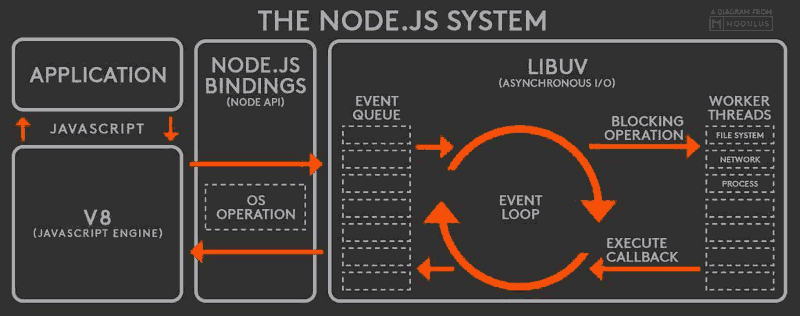
\includegraphics[width=1\textwidth]{assets/nodejs_system.png}}
	\caption{Node.js system}	
	\label{fig:nodejs}
\end{figure}

The main advantages of running a node.js server:

\begin{itemize}
\item{} Node.js server can asynchronously process incoming requests. Therefore the response rate is faster. 

\item{} Node.js is event-driven, and uses non blocking I/O by utilising callbacks, event loop and event queue. This means that we use browser style concurrency model on the web server.

\item{} Since it is javascript we are able to take advantage of the V8 Javascript Engine. V8 Javascript Engine compiles Js code into native machine code which brings better performance comparing to usual techniques such as interpreting.

\item{} Node js is well suited for real time application that run across various devices. It is perfect for fast delivering of data to many requestors at the same time.
\end{itemize}



Figure \ref{fig:nodejsVsTraditional} shows a comparison of request processing on a node server and a traditional web server (e.g. web server Apache). On a traditional web server for each request a new connection thread is created from a limited thread pool or the server waits for any of the working threads to finish so it can delegate the request to them. Many threads use a lot of RAM and the system eventually slows down or even crashes in the case of a lot of requests.
What Node.js does differently is it operates on a single-thread using non blocking I/O calls, which allows it to support a lot of simultaneous connections.
Assume that each request-thread will demand 2MB of memory. Let's also assume that the server is running on an 8GB of RAM. This leaves us with a conclusion that when using a traditional web server it is capable of processing about 4000 simultaneous requests. Node.js in contrary is theoretically able to process over 1M simultaneous requests due to its scalability. \cite{why-node}

\begin{figure}[!ht]
	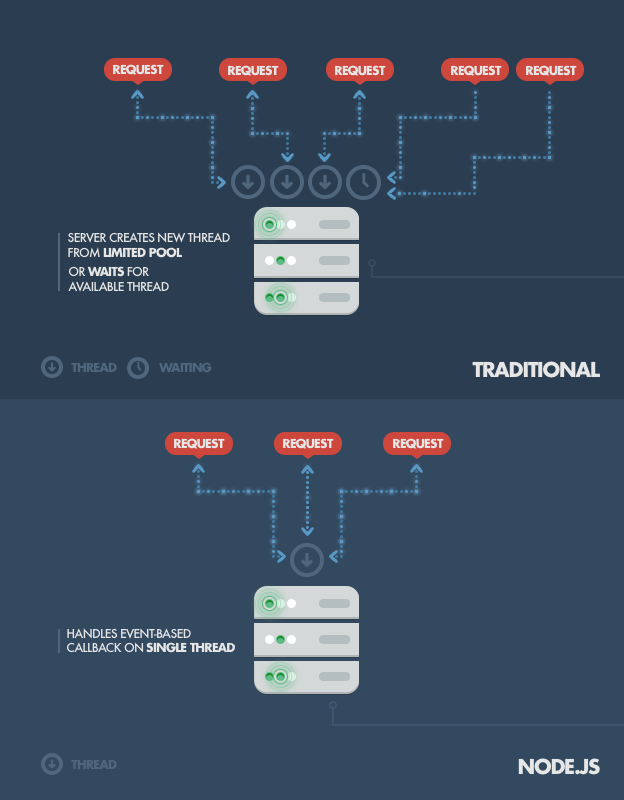
\includegraphics[width=1\textwidth]{assets/nodejsVsTraditional.png}}
	\caption{Node.js server processing compared with traditional web server processing of requests}	
	\label{fig:nodejsVsTraditional}
\end{figure}


\newpage
\subsection{React}
React is a very flexible view layer written in javascript. 
%http://developer.telerik.com/featured/introduction-to-the-react-javascript-framework/
It has many advantages over the existing ways of treating front-end, with the main one being the way it is organised. It breaks down the application into components and makes it very easy to make changes without affecting other code. The components, each of them representing a single view (e.g. a button, form), can be reused for other applications since each component represents an independent part of the programme. This also makes it easy to code and read code since looking at one file tells you how the whole part of the system functions. \cite{react-ant}

It uses a declarative programming style. Declarative programming is when we tell the machine what we want to see as the result and let it figure out how it should be done. \cite{react-fb}

React's way of creating application might not seem correct to many developers since it embeds css and html in javascript, which has been considered a bad practice throughout the past decade. Mixing markup with logic is what we have been always avoiding. However there are quite a few issues with CSS which React JS, due to its approach, solves without any hacks. For instance no need to worry about dependencies, dead code elimination, minification, isolations, etc. Moreover this approach allows us to create independent and easy to read components which can be changed at any time without worrying about affecting the rest of the application.

One of the biggest advantages is the virtual DOM. React does not re-render the whole DOM every time you make a change. React creates a diff between the existing DOM and your changes and applies the patch to the existing DOM, changing only a part of it and saving loads of time.

Server rendering is another very important point. Server rendering allows to render the whole page on the server side (e.g. Node.js), which is faster and SEO-friendly. Both virtual DOM and server side rendering make React's performance very high.

Furthermore React has good descriptive warnings which make the debugging process easy. Its declarative approach makes the code predictable and easier to understand. Therefore the learning curve is flat and developers start making changes with confidence faster. 

React relies on unidirectional data flow. The data, called props in React, are passed from parent to child. When the props change the component is re-rendered in order to keep up to date with the application data changes. Also every component has its own private data called state. \cite{react-ant}\cite{react-fb-native}\cite{react-telerik}

\subsection{ReactNative}

\subsubsection{Why not use Native?}
The native mobile development is difficult and cumbersome. Firstly it is difficult to place different components of your app on the screen since you often need to compute exact positions of all of your views. Moreover every time the developer makes a change in the app they need to recompile the whole application, even if it is the smallest change, such as enlarging fontSize. This takes a lot of time from the development process and slows down the whole development cycle. In the case the developer wants to create a multi platform application, let's say for iOS, Android and Windows, they need to write the same application three times in three completely different languages. Apart from the need to learn specific platform implementation and principles, which are usually not reusable for other platforms, the developer also has to think about memory management, thread concurrency and deployment process. All these issues are important and bring a necessary overhead when developing native applications

Even though development of native applications is a lengthy and difficult process, there are reasons why it is worth it. One of the main reasons why developers go and make native apps is the access to mobile native functions which allow to create a better-feeling experience, such as UI components - date pickers, sliders, etc. This main feature of native development is reproduced in ReactNative as you can read further.\cite{react-fb-native}

\subsubsection{Why ReactNative?}

It is the JS framework which works with mobile's native functions directly, which is it's huge advantage.

React Native runs the code using an interpreter and provides a native bridge to construct and fully interact with platform's native elements. Just like React, which renders divs and spans in the browser React Native renders native higher-level platform-specific components inside of an embedded instance of JavaScriptCore in the application. It also allows to use CSS Flexbox which creates a better User Experience and an easier placement of the elements with no need for computing their position.

Furthermore working with React is faster than with other platform native languages, since you do not have to recompile the whole app any time you make the tiniest change, you just refresh the application and view your changes straight away. Its very handy and it saves a lot of development time. React Native also provides us with the ability of parallelising the work, which increases the speed of the application.

This framework introduces a totally new approach for developing mobile apps and enforces a new principle: 'Learn once, write anywhere'. Facebook provides implementations and supports both IOS and Android versions. Since React Native is a very recent framework it does not fully support native features for both systems. At the moment Facebook has more components and APIs ready for use with IOS than for Android. Android, on the other hand has a lot of open source components which are easily accessible.

ReactNative can be used alongside with the native code. In order to use native code functions the developer has to create a bridge between ReactNative and native and export the functions they want to use in javascript.

The last but not the least, ReactNative uses React, view framework described earlier. \cite{react-fb-native}


\subsection{Objective C}

React Native is a very young framework and it has not been fully developed, not all the native components have been wrapped with javascript in order to use in React Native applications. Therefore using Objective C while developing react native application is one of the conditions when the application requires a little extra functionality.

\subsection{MongoDb}
MongoDb is a non relational database which stores its data in documents. If well designed it provides a very fast way of retrieving data. Among the main advantages over usual RDBMS belong:

\begin{itemize}
\item{Easy structure.} The developer does not need to create difficult relations, foreign keys and relation tables in the schema, since there is no schema. It is a document based database, which holds collections of documents.\cite{mongo-docs}

\item{No complex joins.} When retrieving data you simply ask for a certain document and get all the needed information straight away. It takes just one request to the database to get your data. The documents are usually comprised of key-value pairs by which  are easy to filter.\cite{mongo-docs}\cite{mongo-article2}

\item{Flexible.} It usually happens that some entities populate certain fields and some do not and then the developer ends up with a lot of NULL value fields. Also adding/removing a new field to/from the RDBMS gets very complex, depending on the relations and the data which the database is already filled in with. Mongodb provides incredible flexibility here, since you can just add fields in some documents and do not add them in others. Doing so you eliminate null value fields and also get rid of the problem of adding/removing the field without breaking the whole structure. \cite{mongo-article2}

\item{Easy conversion.} The data in Mongodb is stored in json format, therefore once retrieved it is ready to use, with no need of conversion and mapping between formats and structures.\cite{mongo-docs}

\item{Query ability.} MongoDb uses its own query language which is similar to SQL and easy to learn to those who are familiar with SQL. \cite{mongo-docs}
\end{itemize}

In terms of security MongoDb does not allow sql injection since it does not use Structured Query Language to retrieve data. However it is still vulnerable to NoSQL injections. When querying the document set you can use a string containing a Javascript expression or you can pass a javascript function. Providing a great flexibility it also provides a loophole for attackers. In the case of passing a function if the user input is not properly validated and escaped the attacker can pass various malicious parameters. Therefore the developers have to make sure they take proper care of the user input. Moreover before version 2.4 mongo had a db variable available in the javascript context, which if misused could provide the attacker with a lot of information about document collections. For more information about this issue please refer to \cite{mongo-injection} and \cite{mongo-injection-docs} or have a look at this article \cite{mongo-article}, which contains working examples of malicious code.

%To conclude MongoDB serves best for the systems with a lot of unstructured or semi-structured data which might require frequent schema changes.
 
\subsection{Webpack}
Webpack is a module bundler, a tool which packs the whole application together, translates everything needed to pure javascript, html and css. The bigger your app becomes the more modularised it is. It is a good development approach to break up your javascript application into multiple modules. The code becomes cleaner and easier to read, the loading time of your application also decreases since you do not load everything at once. Webpack takes these different modules with dependencies and merges them serving the content understandable by the browsers. \cite{webpack}

 
\subsection{Augmented Reality}

One of the options this mobile application provides is leaving 3D objects pinned to GPS. In order to implement this I used technology called  Augmented Reality.

Augmented reality is the real world enhanced by the virtual reality. Virtual reality objects are placed in the real world settings and can be viewed with the help of various devices: mobiles, tablets, smart glasses etc.

There are several different types of Augmented reality and it is not within the scope of this thesis to mention and describe all of them. However I would like to mention a few interesting types which I was researching about when choosing which type of Augmented Reality I would use.

\begin{itemize}
	\item{Marker based AR}
	
	The marker was created to help the device overcome the difficulty determining orientation of the camera and  understanding what environment it was observing. The marker is an easily detectable external sign placed on any surface. Once the camera detects and recognises the marker it can define the correct scale and pose of the camera. This technique is commonly known as marker based tracking. Marker can be anything from a clear black and white image to a colour photo. The main condition is that the marker has to be recognisable and not visually merge with the environment surrounding it. Preferably the marker should be a square since four points are enough for the camera to recognise its orientation precisely. Figure \ref{fig:marker} and Figure \ref{fig:marker2} are examples of different types of markers. Each marker can have information encoded in it, which would be identified by the device and further processed, for instance commercials might encode video links, which are played when the marker is recognised. Marker based systems are popular due to their fairly easy implementation and a number of accessible frameworks implementing that functionality out of the box. \cite{ar-research}
	
	\begin{figure}[!ht]
		\centering
		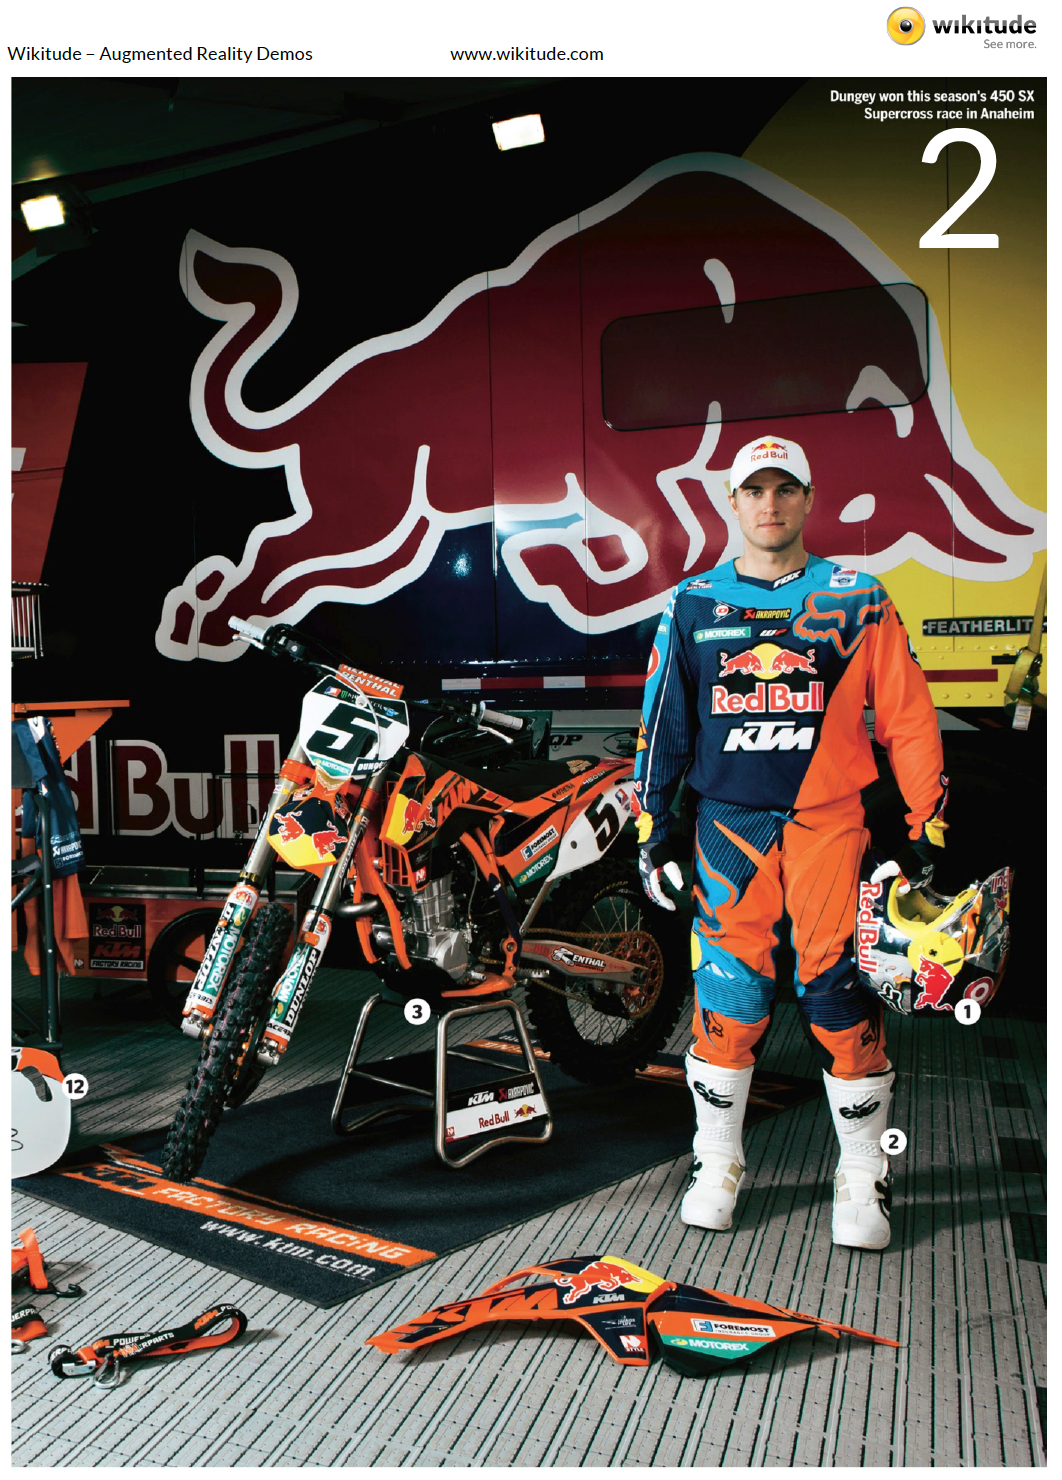
\includegraphics[width=0.5\textwidth]{assets/marker.png}}
		\caption{Photo marker example \\ Source: \cite{wikitude}}	
		\label{fig:marker}
	\end{figure}

	\begin{figure}[!ht]
		\centering
		
\includegraphics[width=0.5\textwidth]{assets/marker2.png}}
		\caption{Black and white marker example \\ Source: \cite{ar-research} }	
		\label{fig:marker2}
	\end{figure}
	
	Marker based AR is implemented in the famous IKEA application which came out in 2014. IKEA made a smart move and made their catalog a marker. The user would place catalog on the floor, point their phone at it and an IKEA piece of furniture would appear.\cite{truong2013today}
	
	\item{Markerless AR}
	
	Markerless Augmented Reality as states the name uses no marker which makes its task more difficult. There are different methods of how to implement markerless tracking but I will only mention the following two as they seem of the biggest interest to me. They are simultaneous tracking and mapping (SLAM) and extensive methods or parallel tracking and mapping (PTAM). Both of these method use no prior knowledge of the environment. Both methods map the environment creating feature maps using various feature detection methods and algorithms. It is not within the scope of this thesis to describe these methods in detail however if interested please refer to \cite{ar-research}. 
	
	\item{Location based AR}
		\begin{figure}[!ht]
		\centering
		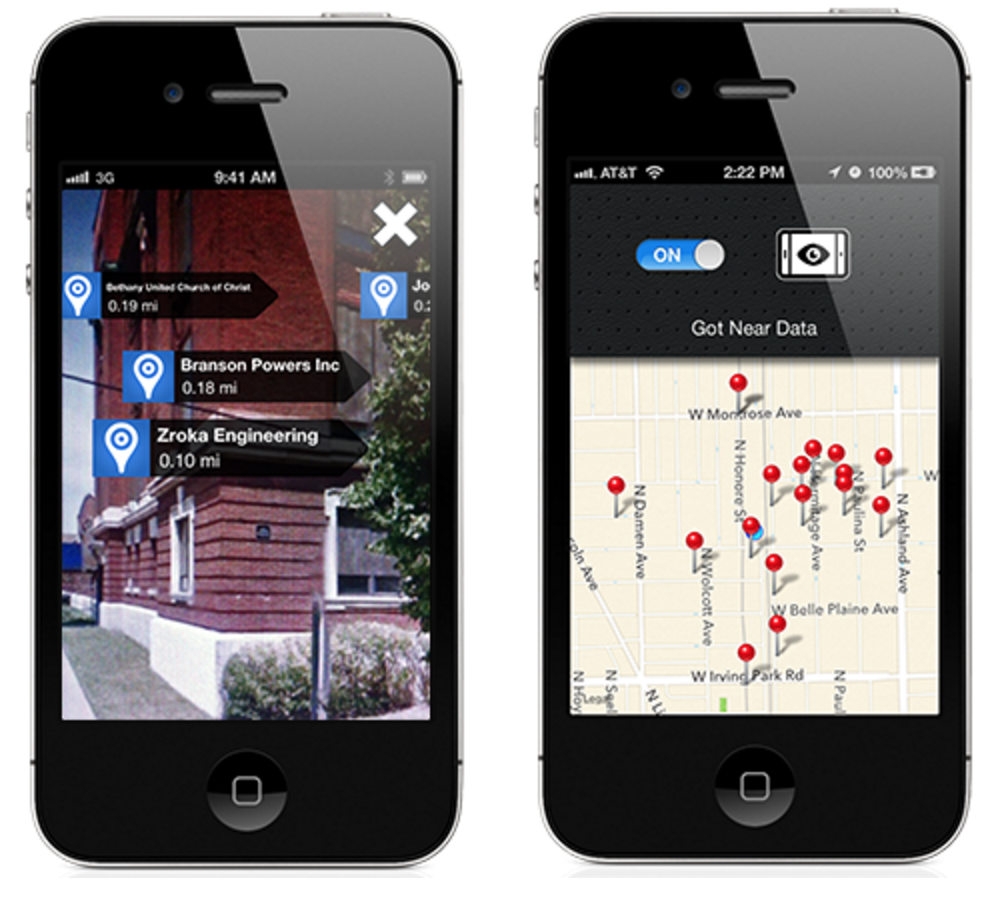
\includegraphics[width=0.7\textwidth]{assets/poi.png}}
		\caption{Points of interest \\ Source: \cite{ar-github} }	
		\label{fig:poi}
	\end{figure}
	This type of Augmented Reality places objects in real world on the pre-defined GPS coordinates. There are several subtypes for location based Augmented Reality: 
	\begin{itemize}
	\item POI or Points Of Interest is when an application registers a list of points of interest and shows them to the user based on his location. For instance it could be different restaurants or shops in the area. Figure~\ref{fig:poi} shows a sample application with POI AR.
	\item Placing of 3D objects. This type is similar to POI but instead of 2D markers on the screen it uses 3D objects which are placed on the given GPS coordinates. Depending on the implementation some object are interactive while others are only for observation. 
	\end{itemize}
\end{itemize}

Augmented Reality can be interactive with user clicking on links and objects to get more information about the scene, product or a building. 

\section{System design}
The goal of the thesis is to create a messaging system which will comprise of a mobile application, web application, server and a database. Figure \ref{fig:system} shows the proposed system's design. As the figure states the core of the system is a Node.js REST API server. It stores data in a NoSQL document database mongodb. Web application will be implemented in React and will be communicating with server through its API. Mobile application will also communicate with the server through API and will be implemented in React Native. The request load is expected to be high due to the system's purpose - messaging. Therefore Nginx http server will be configured as a load balancer using strategy least connectivity for helping to deal with requests. Least connectivity strategy forwards the incoming request to the server with the smallest number of connections. %SOURCE
	\begin{figure}[!h]
		\centering
		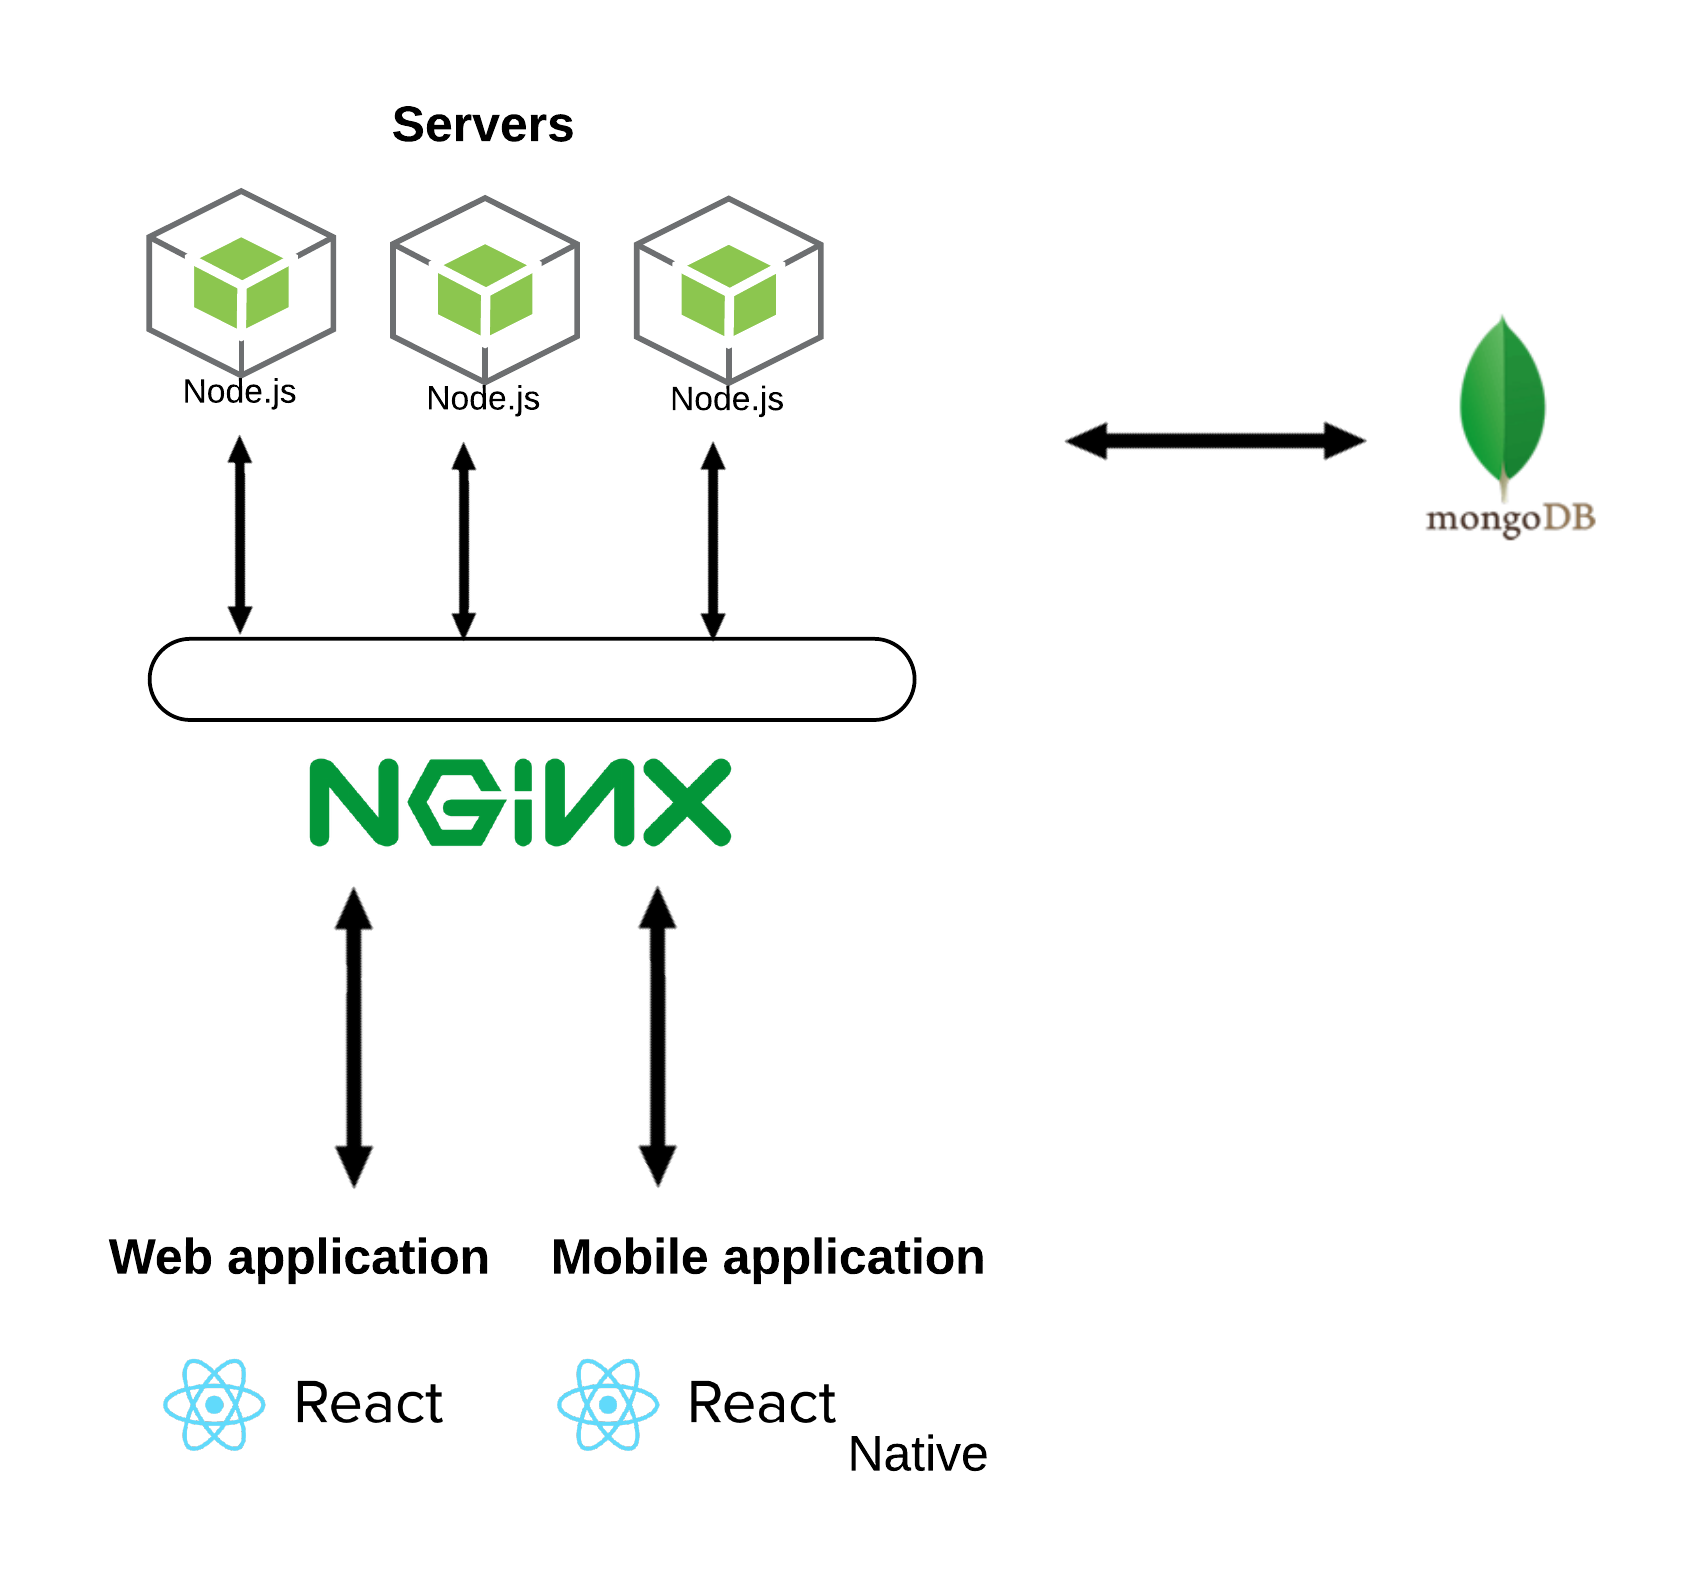
\includegraphics[width=1\textwidth]{assets/system.png}}
		\caption{Interaction between parts of the system  }	
		\label{fig:system}
	\end{figure}

\section{Database}
One of the most important parts of any application is the database design. It is essential to understand how your data will be handled, saved and organised before starting to build an application. As was already mentioned in the previous chapter I chose MongoDB for this implementation. MongoDB does not define a scheme design principles or design notation which I could use. Therefore I used a simple notation where each square element represents a single collection as the figure \ref{fig:model} shows. The arrows are the references, the way where the arrow is pointing the reference is provided.

MongoDb has a different view on data than relational databases. Relational databases are focused on what answers we have when document based databases are more focused on what questions we have. Therefore minor duplications are allowed, because they will save time preventing the database performing joins and looking up information in other tables.

In GPS pinned application the main concern is the messages. We need to know on one request what is the message and all details about it. 
\begin{itemize}
\item Message

Message contains all the necessary data about the message. The message document contains message text, description, which is a 150 characted substring of text, its location with latitude and longitude and also city and country, which will be populated based on the Google Api response using coordinates. The message also contains object user with user's id and username. The case is that when previewing the message the only information we need to show the user is the username of the person who left the message. This minor duplication saves us time we would have spent looking through the user table in order to find correct user and get his username. MongoDb being a document database allows us saving the image as a base64 string right into the document. Maximum size of the MongoDB documents is 16 MB. We are dealing with mobile phone pictures which are on average between 2 and 5MB so we don't need to worry about space. %SOURCE! 
Just for the information in case of bigger images it is also possible to save them in the collection. MongoDb has a tool which splits big documents in several smaller allowing any size to be safely saved in the collection.  %SOURCE

	\begin{figure}[!ht]
		\centering
		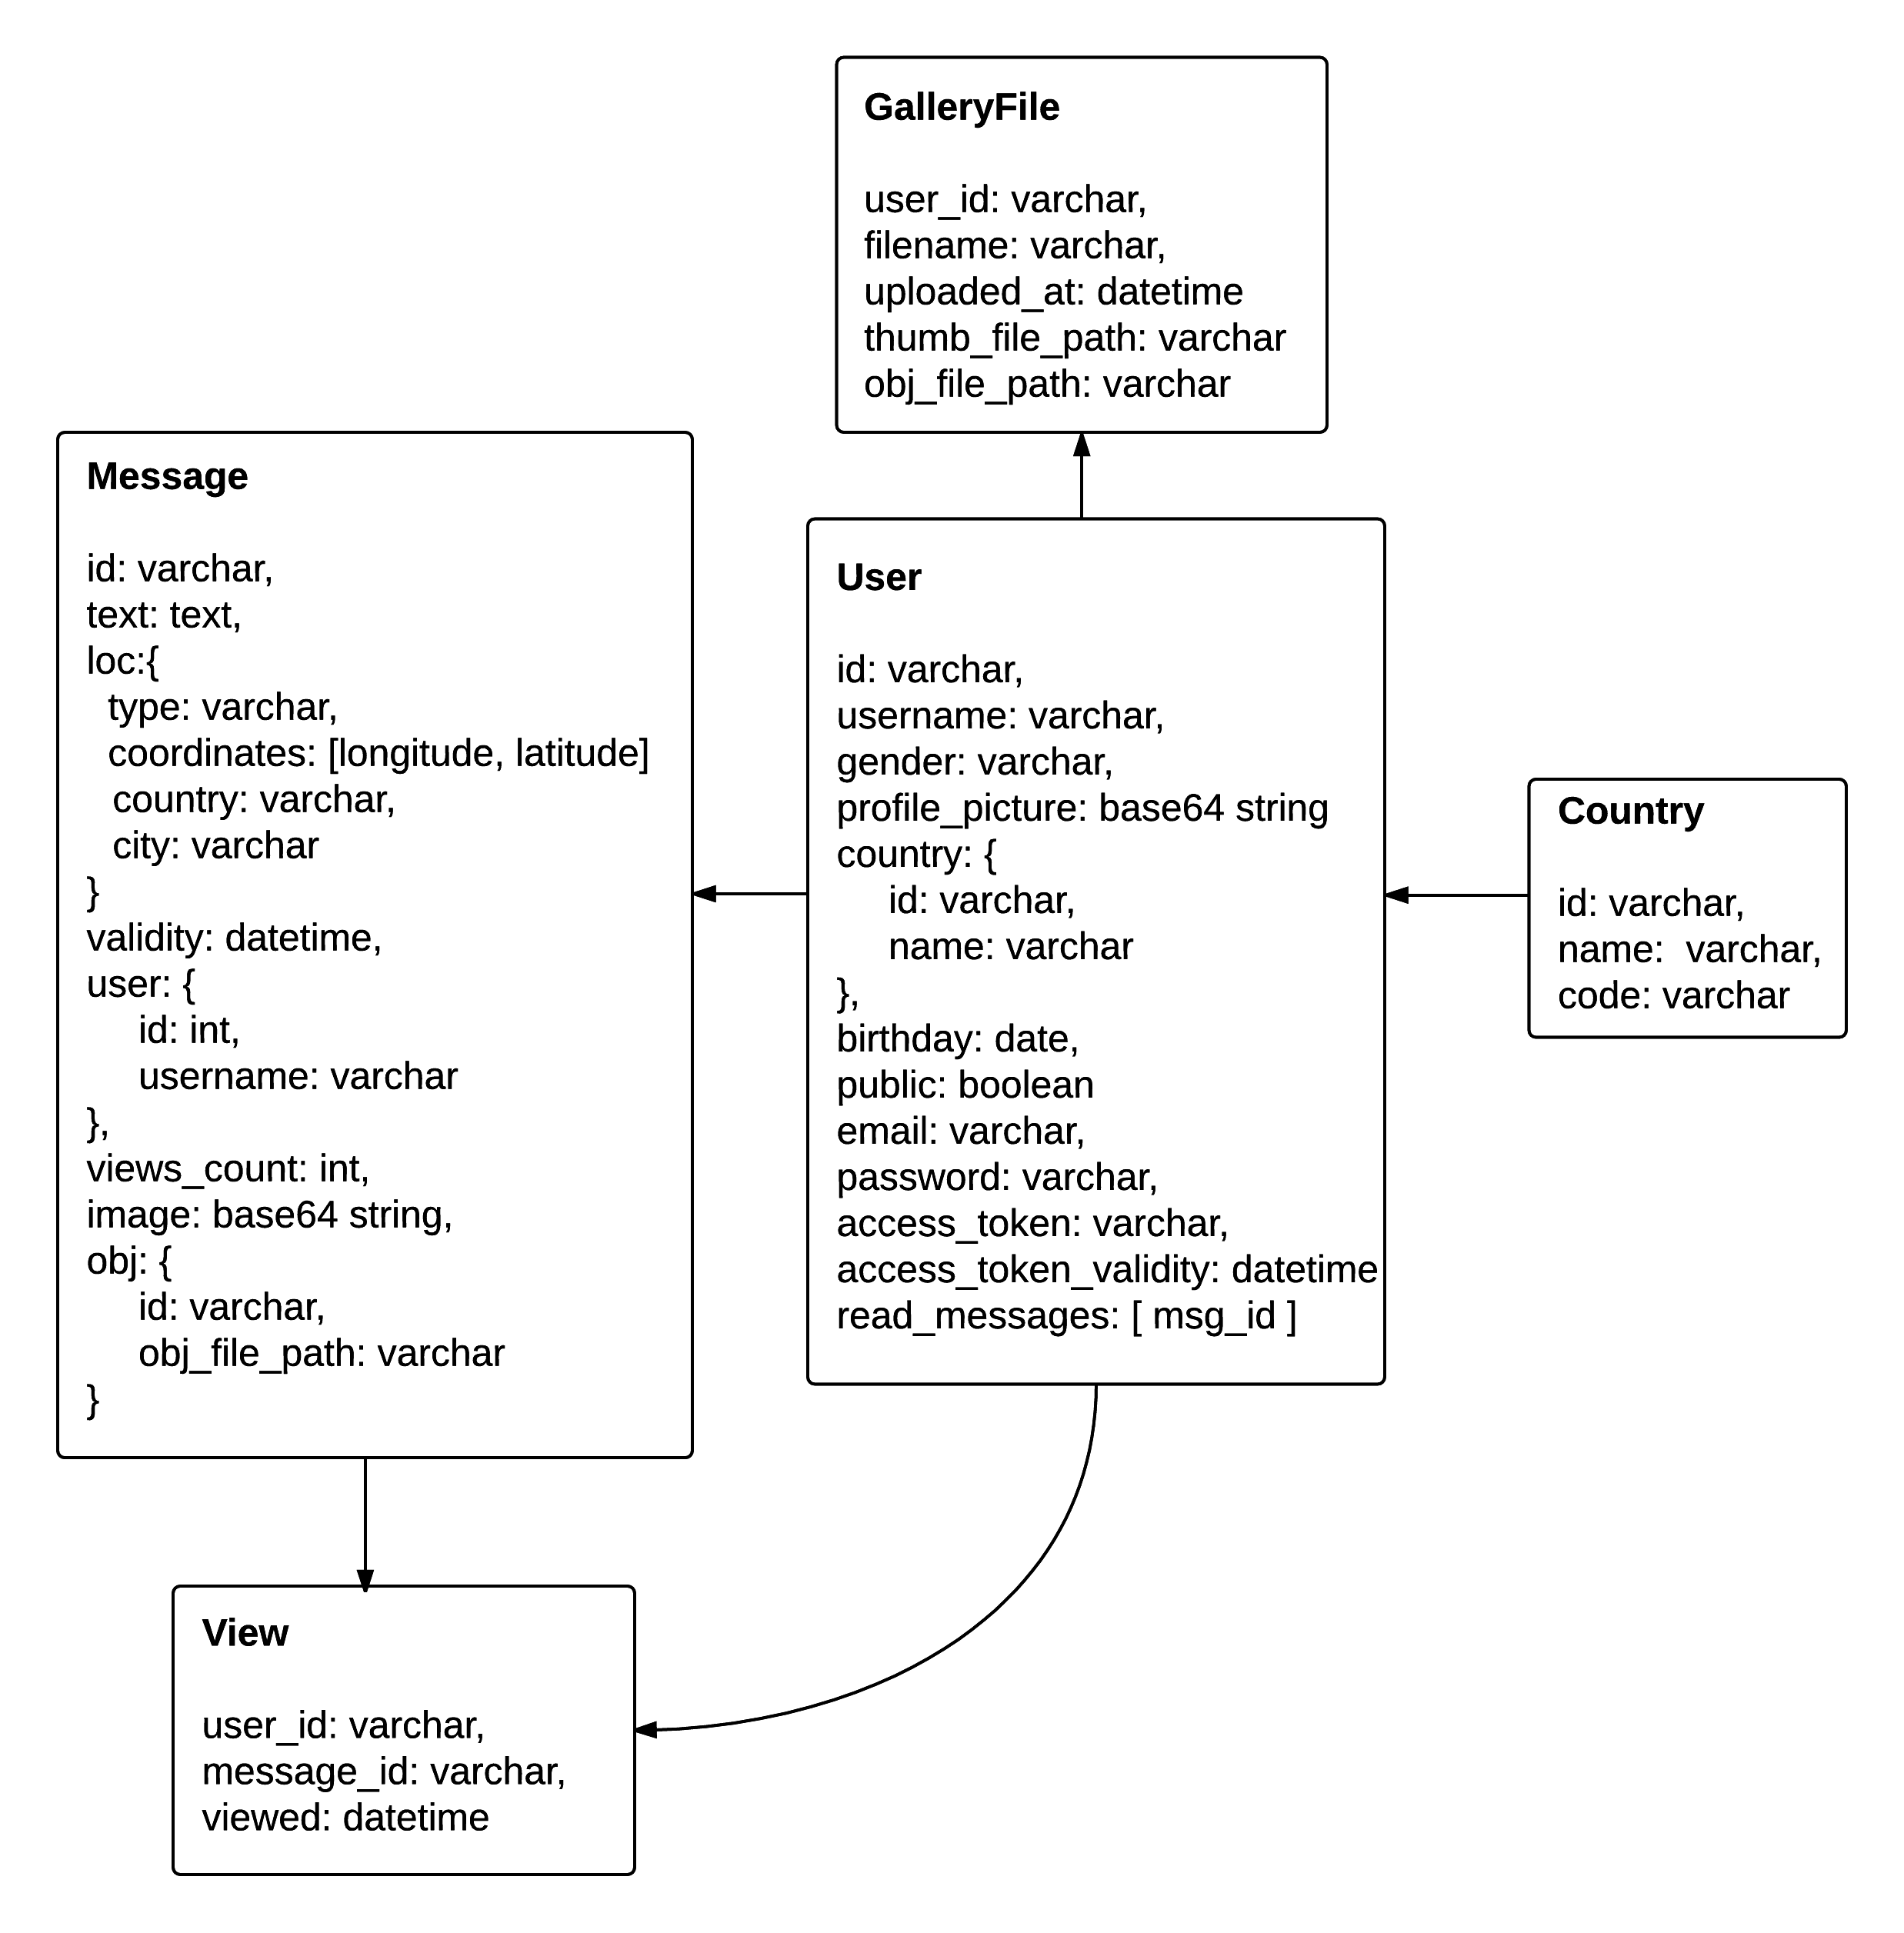
\includegraphics[width=1\textwidth]{assets/model.png}}
		\caption{MongoDB model of GPS pinned messaging application }	
		\label{fig:model}
	\end{figure}

Some messages will be 3d obj and in order to save time and server side operations object id and its path will be saved directly in the message document.

\item User

User document contains standardised user data, authentication fields and a profile picture. User document also has a country string saved in it. The country list is saved in a json file and is provided to the user as a dropdown select in the mobile application.

\item GalleryFile

Every user will have their own object gallery. They can upload their 3d object there according to the instructions given on the web. There will also be a common gallery from which users can choose objects they like and add them to their gallery. User gallery objects will have field user id populated while common gallery objects will have that field set to null. Each object will have a thumbnail and an actual file paths saved.

\item View

This collection will have info about when and which user viewed which message. This collection will be used for statistics and when checking for new comments and views of users messages.


\item AccessTokens

Access tokens are generated on the server side and are connected with a user and a client.

\item RefreshTokens

Refresh tokens are used for regaining an access token after it expired.

\item Clients

Clients documents is a list of client application communicating with the API. 

\end{itemize}


\section{Augmented Reality Feasibility study}
\label{section:ar}

After conducting a thorough research concerning various Augmented reality implementations, techniques and frameworks I limited my options to three choices. My goal is to be able to place a 3D object at a given GPS location. Therefore I was looking for a location aware solution. Below are listed different AR solutions I was considering.

\begin{itemize}
	\item{Open source Augmented Reality SDK}
	
	There are a few open source AR SDKs with IOS support, implemented in Objective C. The one which seemed to be the most relevant can be found at  \cite{ar-github}. This is a neat small framework which supports even the older iPhones. It supports a type of AR called POI or Points Of Interest. It is well documented and has a video tutorial on how to get started with the framework. There are also well commented code and a sample application.
	
	Advantages:
	\begin{itemize}
		\item{Support for Points of Interest} therefore Geo location support.
	\end{itemize}
	
	Disadvantages:
	\begin{itemize}
		\item{No support for 3D object. The developer would have to implement 3D object rendering himself.}
		\item{Implemented in Objective C, which is not the most developer friendly language.}
		\item{The last update of the framework was performed 2 years ago. The framework is not supported anymore. There is no community and in case of problems or bugs the developer has to deal with everything himself. There is an option of communicating with the author, but he didn't respond to my email inquiring about the possible support of 3D images, so I would not rely on that.}
	\end{itemize}

	\item{Unity 3D - Kudan AR plugin}
	
	Kudan is an Augmented Reality SDK.  Kudan supports iOS, Android and Unity cross platform game engine. It claims to offer a much better Augmented Reality experince using its Advanced tracking for both marker and markerless augmented realities then the existing frameworks. For more information about Kudan please see official website at \cite{kudan}.
	
	Advantages:
	\begin{itemize}
		\item{SLAM} - Simultaneous localisation and mapping is a great technique displaying 3d objects. It has already been shortly described in the previous chapter. The beauty of it is that it maps the environment and puts the object in it so it looks natural. For instance if your camera would be facing a table the object will be put on the surface of the table.
		
	\end{itemize}
	
	Disadvantages:
	\begin{itemize}
		\item{SLAM} - even though it is an advantage, it is also a disadvantage since for my purposes I need to have an object placed at a certain location. Unfortunately it is not possible with SLAM since it is not a location based technique. Therefore when using SLAM and turning the camera around, the object will always stay in front of the camera, which is an unwanted result for me.
		\item{New framework} - it is not a severe disadvantage, but usually new frameworks tend to be buggy. It is better to wait some time until the next version is released to start using any new system.
		\item{Resource changing} - the mobile application is supposed to serve the url of the AR object to render. Kudan Unity plugin did not offer an easy and pretty way of doing so. With Kudan serving new AR object would involve physical moving of files and recompiling which would not be possible in my application.
	\end{itemize}	
	\item{Wikitude AR}
	Advantages:
	\begin{itemize}
		\item{Javascript API} - Wikitude provides a clean API with good documentation. It is a huge advantage since the main technologies I am using in my thesis are all javascript based.
		\item{Big community and support} - The Wikitude AR has a big community and a forum with a lot of different issues to browse through. It has been already developed for several year, which means loads of useful features were implemented and bugs eliminated.
		\item{iOS integration} - My application starting point is objective C project and I was looking for a solution which would be easily integrated in Native - React Native flow. The documentation provides with a good example of how to work with the Wikitude.
		\			
	\end{itemize}
	
	Disadvantages:
	\begin{itemize}
		\item{Trial version} - the only available version to use is a free version, however with full support of all SDK's features, is trial. There is a watermark on the camera screen when using AR.
	\end{itemize}		
\end{itemize}

The first option did not seem to be suitable as it would require deep understanding of Objective C in order to implement rendering and fix possible problems which might arise during development. The focus of this thesis is to explore new ways of creating applications such as using javascript wrappers for objective C to create pure native experience. Moreover this thesis is taking advantage of different other javascript techniques and I would mainly want to focus on possibilities offered by javascript frameworks.

The second option Augmented Reality wise is a good choise, but it doesn't support location awareness and brings a lot of difficulties when trying to serve it with new resources.

After careful consideration I decided to choose the Wikitude AR SDK with trial version. It seems to be the best solution, not minding the trial flags on the camera. It provides an easy way of integrating the framework in my application. Javascript API is also a very big advantage.



\chapter{Realisation}

\section{Server}


The server is implemented as a REST API Node.js server using Express framework. Express is a commonly used base for a server. It includes the main components and libraries the developer needs to create a server. It is a minimalistic framework that serves as a solid starting point, providing a robust set of features, middleware and methods. It makes creating API quick and easy. Many frameworks created for working with Node.js are based on express. Express is even shipped with a generator which provides you with a basic directory structure. Detailed info about the framework, including documentation and examples can be found at \cite{express}. 
\subsection{Endpoints}
REST API design is an important part of the realisation process. It helps defining application's functions and capabilities and develops an overall understanding of the workflow.

\begin{itemize}
\item{Index}
	
	 \verb GET  \url{/}	
	
	renders API documentation	\\
\item {Messages}

	 \verb GET  \url{/messages?lat=''&lng=''} 
		\begin{itemize}
			\item \verb|lat| - latitude coordinate
			\item \verb|lng| - longitude coordinate		
		\end{itemize}	
	
	retrieves all messages within the preset radius of 50 meters from the given location specified by latitude and longitude \\~\\
	
	 \verb POST  \url{/messages}	
	
	saves a message to the database	\\~\\
	
	 \verb GET  \url{/messages/:id}	
		\begin{itemize}
			\item \verb|:id|	- message id, string
		\end{itemize}		
	
	returns a message with the given id		\\~\\
	
	 \verb GET  \url{/messages/user/:id?page=''&limit=''}	
		\begin{itemize}
			\item \verb|:id| - user id, string
			\item \verb|page|
			\item \verb|limit|
		\end{itemize}		
	
	returns user's messages, supports pagination	\\~\\	 
	
	 \verb GET  \url{/messages/:id/comments?page=''&limit=''}	
		\begin{itemize}
			\item \verb|:id|	- message id, string
			\item \verb|page|
			\item \verb|limit|
		\end{itemize}		
	
	returns message's comments, supports pagination \\~\\	 
	
	 \verb POST  \url{/messages/:id/comments}	
		\begin{itemize}
			\item \verb|:id|	- message id, string
		\end{itemize}		
	
	saves a comment for a message specified by id \\

\item {Files}	
 
	 \verb|POST|  \url{/files/form}	
	
	special endpoint for saving the web form for uploading gallery images \\~\\	 
	
	 \verb GET  \url{/files/gallery?page=''&limit='}	
		\begin{itemize}
			\item \verb|page|
			\item \verb|limit|
		\end{itemize}		
	returns common gallery files, supports pagination \\~\\	 
	
	 \verb GET  \url{/files/gallery/user/:id?page=''&limit='}	
		\begin{itemize}
			\item \verb|:id| - user id, string
			\item \verb|page|
			\item \verb|limit|
		\end{itemize}	
	returns gallery for the user, specified by id,  supports pagination \\
	
\item {Users}	
 
	 \verb GET  \url{/users/me}	
	
	returns information about the currently authenticated user	\\~\\	 
	
	 \verb GET  \url{/users/:id}	
		\begin{itemize}
			\item \verb|:id|	- user id, string
		\end{itemize}		
	returns information about the user specified by id \\~\\	 
	
	 \verb POST  \url{/users}	

	creates a new user \\~\\	 
	
	 \verb PUT  \url{/users/:id}	
		\begin{itemize}
			\item \verb|:id|	- user id, string
		\end{itemize}		
	updates information about the user specified by id	\\
\item {OAuth} 

	 \verb POST  \url{/oauth/token}	
	 
	 Request body content-type is \verb application/json   and it must contain
		\begin{itemize}
			\item \verb|client_id|
			\item \verb|client_secret|
			\item \verb|username|
			\item \verb|password	|								
		\end{itemize}		
	
	If username and password are correct the endpoint returns a token for authenticated communication with the server.
\end{itemize}
	All of the above listed endpoints are only accessed with a valid token with exception of the index which provides documentation.
	
\subsection{Authentication}

One of the functional requirements for the server is to provide authentication for users. The authentication will be implemented using OAuth 2 protocol. It fits well our needs because we will be communicating with our server through API from two different applications. Figure \ref{fig:oauth} demonstrates OAuth 2 authentication flow. There are 3 main actors in the authentication process.

\begin{itemize}


\item User

The user owns a resource which an application wants to access. In the case of authentication the resource is user information, their credentials and personal information. The 3d party needs to access it in order to identify and authenticate the user.

\item Service API

Service API is an Authorisation and a Resource Server. It hosts user protected information and verifies the identity of the user so it can provide the client application with an access and refresh tokens to communicate with the server.

\item Client

The client is an application which wants to access user information and other resources which user allows it to use. Before the application is able to access any of that information the user has to authorise it's activity.

\end{itemize}

The authentication flow is the following:

\begin{enumerate}
\item The client application sends the user an authorisation request asking them to allow permission to access their information. It usually appears as a new window, where the application shows the user a list of information it wants to access.
\item In the case that user agrees he provides the client application with an authorisation grant, which is used for further verification of user's identity
\item The Client application uses obtained authorisation grant to form another request to the Authorisation/Resources server, which contains it's client id, client secret, authorisation grant type and the details of authorisation grant sent by user.
\item If the server identifies the client application and the user it issues a response which usually contains an access token, a refresh token and a token expiration date. Authorisation process is complete at this stage. Both client and user were verified by the server.
\item Once application has the token it can issue requests to server to access protected resources which belong to the user.
\item If the client application sends the correct token it is granted access to protected resource. In the case the token has expired the client can always use refresh token in order to receive a new access token.
\end{enumerate}

There are several different authorisation grants that are supported by OAuth 2. It is not within the scope of this thesis to discuss all of them however if interested please refer to \cite{oauth}. The Password authorisation grant was chosen for authentication with the server. It requires the user to provide the client with their username and password. This grant should only be used in the case when the application is trusted by the server such as our case, when both applications and the server are created as one system.

In order for this whole process to work the client application has to be previously registered with the Authorisation/Resource server. After the registration it will receive a client id and a client secret or so called client credentials which are used for authenticating with the server.

Example of the request with authorisation grant which is described in the step 4 is showed below. \\~\\
\verb|POST| \url{https://oauth.example.com/api/oauth/token} \\ Request body:

\begin{lstlisting}[language=JavaScript]
{
    "grant_type": "password",
    "client_id": "public_client_id",
    "client_secret": "very_secret_client_secret",
    "username": "mark",
    "password": "secretpassword"
}
\end{lstlisting}


\begin{figure}[!ht]
	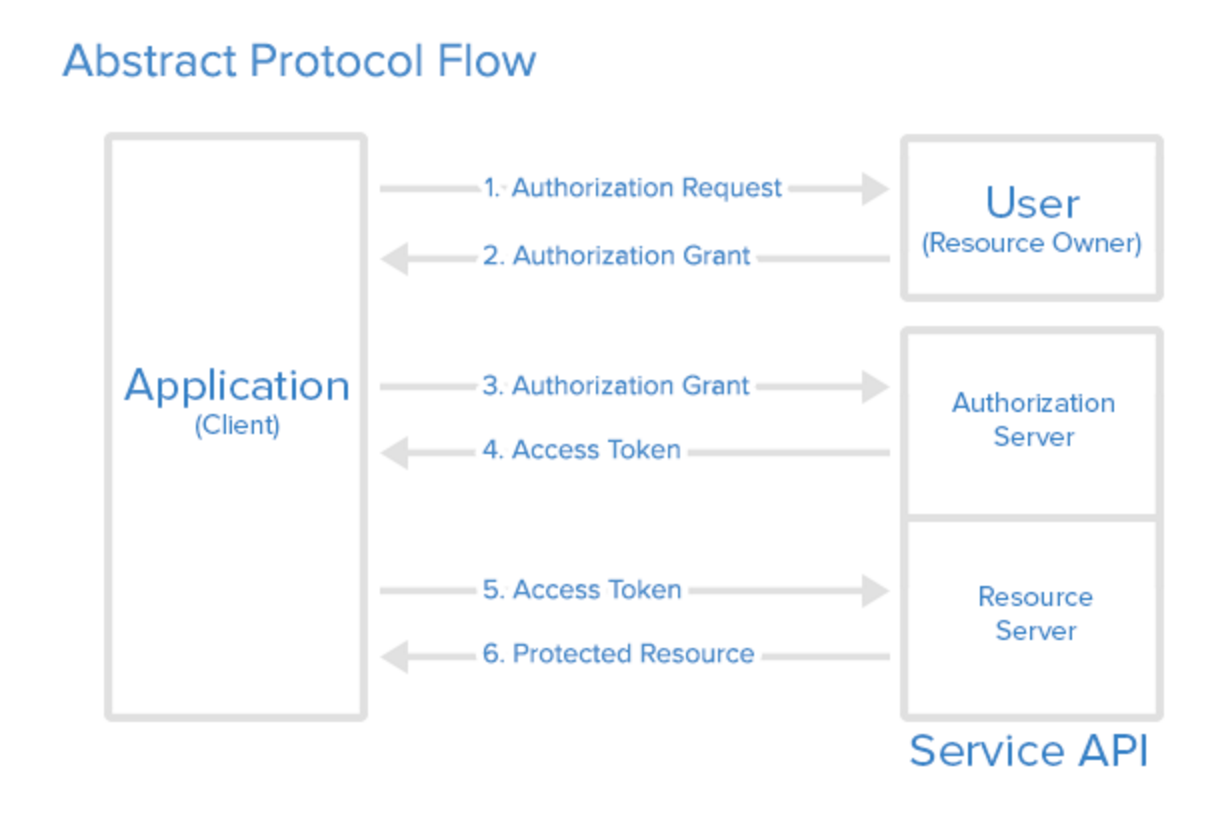
\includegraphics[width=1\textwidth]{assets/oauth.png}}
	\caption{OAuth2 authentication protocol flow. \\ Source: \cite{oauth}}	
	\label{fig:oauth}
\end{figure}

\subsection{Files processing}

The server is working with files attached to the messages, 3d objects and their thumbnails. 

Web application will have a form which will be used for uploading 3d objects and their thumbnails to the server. The application will be sending a request with content type  \verb|multipart/form-data| which needs to be parsed in order to retrieve information and files from it. Node.js offers a number of handy middleware which parses \verb|multipart/form-data| and works with files. After a thorough research I chose \verb|node-multiparty| available at \cite{multiparty}. This library parses the form data and makes files attached accessible. 

Thumbnails for 3d objects have to be resized to smaller size not to waste space on the server. For resizing  a \verb|node-imagemagick| library available at \cite{node-imagemagick} was chosen, which uses original \verb|ImageMagick| library availble at \cite{imagemagick}.

Message attachment files which are not objects are resized on the side of the mobile application. Therefore no further server side processing is needed. 

\subsection{Distance and radius retrieval}

One of the main functions of the server will be returning messages within a given radius of user's current GPS location. The calculation of the distance from the user's GPS location will be done using sphere geometry.

In the case of distance calculation there are two ways one can choose - either using Euclidean geometry or spherical geometry. Euclidean geometry is also known as the 'plane geometry'. It is a type of geometry where the internal angles of triangles add up to 180 degrees, parallel lines do not ever cross and everything is flat. Spherical geometry on the contrary does not take account of flat world and works with 3d. Since the earth is shaped in a form of a sphere it would be better to use spherical geometry for distance calculations, since they will be more precise.
%SOURCE

The messages endpoint returns messages within the preset radius from given GPS coordinates. Retrieval of messages needed to be fast and effective with the expected growing message collection. Simple search with comparing distances between given GPS and message's location was not suitable. 

MongoDb has a powerful system of geo queries. It supports both 2d and sphere geo queries. To use these queries document data have to be saved in GeoJSON format. Documents in this format consist of an array of coordinates (longitude, latitude) and a type. There is a vast selection of types such as for instance "Polygon" or "Geometry Collection". My geo location data are representing a single point therefore I chose type "Point". The example of data in preferred GeoJSON format is shown below.

\begin{lstlisting}[language=JavaScript]
"loc" : {
    "type" : "Point",
        "coordinates" : [
        14.422061,
        50.087657
    ]
}
\end{lstlisting}

The following is an example of geo query. Another optimisation of search performance is creation of a 2dsphere index on location field.

\begin{lstlisting}[language=JavaScript]
loc: {
    $geoWithin: {
        $centerSphere: [
            [
                longitude,
                latitude
            ],
            radius
        ]
    }
}
\end{lstlisting}

This is a simplified example of mongoose message model with index definition. The actual example of the model is more complicated and can be found in the server implementation in folder \verb|models| under name \verb|message.js|.

Firstly you include \verb|mongoose| library on line 1 and define Schema on line 2. Specific schema definition follows on lines 4 to 9. The line 11 defines index \textit{2dsphere} over \verb|loc| field of the model. Lines 12 and 13 register and export the model.
 
\begin{lstlisting}[language=JavaScript]
var mongoose = require('mongoose');
var Schema = mongoose.Schema;

var messageSchema = new Schema({
        loc: {
            coordinates: {type: [Number], required: true},
            type: {type: String, required: true}
        }
    });
messageSchema.index({loc : '2dsphere'});
var Message = mongoose.model('Message', messageSchema);
module.exports = Message;
\end{lstlisting}


\subsection{Load balancer}

Among the non functional requirements there are Scalability and Performance. In other words the server has to be able to cope with growing requests load and it should be easily scalable if needed. Using load balancer fulfils both of these requirements. Load balancer will forward requests to the chosen server instance in case others are too busy to process new requests. Scalability of the server can be achieved with running more instances and configuring load balancer to register these new server instances.

Load balancer I used is called \verb|Nginx|. It is an http server but is also a reverse proxy server and used for load balancing. Load balancing strategy used on the server is \textit{least connectivity}. \textit{Least connectivity} strategy means that the server with the smallest number of connections will receive new request. \cite{nginx-lb} Another advantage of having nginx taking care of incoming requests is that it can also take care of serving static content instead of the actual server. 

The main part of the Nginx configuration file with registered load balancer is showed below. It is preferable to use \textit{ssl} connection for running the server. The example contains configuration for connecting over \textit{ss}l and without. Lines 3 to 8 of the configuration file define the upstream, the servers which will be processing incoming requests. The load balancing strategy is defined on line 4. Lines 13 and 14 indicate path to log files. The static content serving is configured on line 16. Line 20 defines the proxy pass, which name matches name of the upstream. This configuration allows all requests coming to \url{http://127.0.0.1:8080} be forwarded to one of the server from upstream according to \textit{leact connectivity} strategy. The configuration on lines 27 to 34 does the same but for the secure connection via \verb|https://| .


\begin{lstlisting}[language=JavaScript]

http {
    upstream air_servers {
        least_conn;                 # Least Connections strategy
        server 127.0.0.1:3000;      # NodeJS AirServer 1
        server 127.0.0.1:3001;      # NodeJS AirServer 2
        server 127.0.0.1:3002;      # NodeJS AirServer 3
    }

    server {
        listen       8080;
        
        access_log /var/log/nginx/access.log;
        error_log  /var/log/nginx/error.log error;

        location ~ ^/(images/|img/|javascript/|js/|css/|stylesheets/|flash/|media/|static/|robots.txt|humans.txt|favicon.ico) {
             root /path/to/static/files;
        }        

        location / {
            proxy_pass http://air_servers;
        }
    }

    # HTTPS server
    
    server {
        listen 443;
        
        ssl on;
        ssl_certificate     /etc/ssl/example.com/example.com.crt;
        ssl_certificate_key /etc/ssl/example.com/example.com.key;

       # plus the same configuration as above
    }
}


\end{lstlisting}


\subsection{Queue}

Priority job queue was used in this project to solve the following problems. 

Firstly when creating a new message the user has to set message's validity in days, from 1 up to 365 days. When a message is created it is valid immediately and becomes invalid after the validity time expires. I was looking for a way to set the valid flag to false when the message expires. Job queue seemed like the perfect solution. 

Secondly I needed to update message's location details with city and country for the statistics endpoints. This involved calling The Google Maps Geocoding Api \cite{maps-api}, waiting for response, parsing the response and updating the document in the database. This slightly lengthy process could not take part while saving the message as it would affect user experience negatively and the application could seem slow. Furthermore in the case of potential problems which could arise from calling 3d party API the whole message saving process could be sabotaged.

\subsubsection{Kue}

Kue is a very simple priority job queue backed up by Redis and created specifically for node.js .

"Redis is an open source (BSD licensed), in-memory data structure store, used as database, cache and message broker. It supports data structures such as strings, hashes, lists, sets, sorted sets with range queries, bitmaps, hyperloglogs and geospatial indexes with radius queries. Redis has built-in replication, Lua scripting, LRU eviction, transactions and different levels of on-disk persistence, and provides high availability via Redis Sentinel and automatic partitioning with Redis Cluster." The description of Redis is taken from its official website found at \cite{redis}

The complete documentation for \verb|kue| is available at \cite{kue}

\subsubsection{Configuration}

Kue as every job queue needs to have consumers and producers created. The producer part of the code was put in the processing of message POST request. Here is the example of the producer code. 

\begin{lstlisting}[language=JavaScript]
function addToValidQueue(queue, message){
    var job = queue.create('valid-queue', {
            title: 'unset valid',
            message_id: message.id,
        })
        .delay(message.validity)
        .save(function (err) {
            if (err) {
            	log(err);
            }
         });
}
\end{lstlisting}


I created a \verb|queue.helper.js| which took care of putting jobs in the queues. There are two queues for two types of jobs: 'valid-queue' and 'geo-queue'. Valid flags jobs had to be delayed so they had set delayed time period calculated from the number of valid days input by the user. The delaying of a job is part of the kue and is implemented by using \verb|delay()| function on line 6 in the example above. I also created two consumers - \verb|geoConsumer.js| and \verb|validConsumer.js|. The example of geo consumer is showed below. The \verb|geoCode| function in the example on line 5 further processes received job data.

\begin{lstlisting}[language=JavaScript]
var kue = require('kue');
var queue = kue.createQueue();

queue.process('geo-queue', function (job, done) {
    geoCode(job.data, done);
});

\end{lstlisting}

\subsection{Supervisord}
 
Nodejs server needs supervision and fast recovery in the case it fails. For this reason I needed a tool which would keep my server running and restarts it in the case of fatality.

Supervisor is client/server system that allows easy monitoring and manipulations with UNIX processes. It has a very detailed and well readable documentation available at \cite{supervisor}. Once started it runs as a daemon process. It also has a command line utility for easy manipulation with processes. They can be restarted, stopped or started from the command line. To specify the programs one needs to run the configuration file is created. Below is showed an example of configuring a server to run. The full configuration file can be found in Appendix \ref{apx:supervisor} \\

\begin{lstlisting}[language=C]
[program:airServer]
directory=/server/directory
command=npm start
autostart=true 
stdout_logfile=/logs/server_out.log
stderr_logfile=/logs/server_err.log  
\end{lstlisting} \\
Queue consumers were also added to the supervisor configuration. 

Supervisor provides standard output and error logging, which eliminates the need to setup a logging flow yourself.

\subsection{Libraries used}

I have used the npm package manager for taking care of the dependencies in the project. Among all the libraries I have used there are a few I would like to mention.

\begin{itemize}
	\item \textit{Passport} 
	
	It is a middleware used for authenticating requests. It uses so called strategies to define different authenticating techniques. There is around 300 strategies including authenticating through social networks and enterprise generation and more. \cite{pass}
	\item {Async}
	
	Async is a powerful library providing functionality for working with asynchronous Javascript. Working with asynchronous functionality get tedious sometimes and this library helps to make it easy. You only need to provide your asynchronous function with a callback which will symbolise its completion.\cite{sync}
	
	\item {Babel}
	
	I needed a compiler to transform some of the Javascript syntax that I was using, for instance JSX  and ES2015. Babel supports latest versions of Javascript using syntax transformers. This lets developer use new features before the browser support comes out. \cite{babel}
	
	\item{Mongoose unique validator}
	
	This small library is extremely helpful. It is connected as a middleware to a model in which unique indexes are defined. Mongoose unique validator does a great job in returning readable and user friendly validation messages. MongoDb unfortunately fails drastically in this. Its validation messages have to go through some serious parsing and analysing before being used. \cite{mvalid}
\end{itemize}

\subsection{Structure}

The directory structure of the server is shown on figure \ref{fig:server_dir}. The base for this structure was generated by the Express directory generator. 

The main logic happens in \verb|app.js|, which defines the whole server, includes important dependencies and connects routes.
The \verb|route| folder describes different endpoint operations. The endpoints in \verb|route| folder use helpers from \verb|util|. 

% source - mongoDb flexibility, changing schema on the fly
The \verb|models| folder consists of \verb|mongoose| models. \verb|Mongoose| is an ORM wrapper for talking to MongoDB. MongoDb is very flexible and does not enforce the developer to have a database scheme defined however it is easier and better to have at least defined models for different collections. Mongo allows changing 'database scheme' on the fly, by adding new keys without any overhead. This advantage might serve as a weak point for an attacker in the case models are not defined, which could allow unwanted and unexpected malicious values get in collections.

The \verb|views| folder consists only of one view because our server serves strictly as a REST API server. The only template shows server's API documentation on the index page.

The \verb|controllers| folder consists of two authorization controllers. The \verb|auth.controller.js| defines authorization strategies of library \verb|passport| such as \textit{BasicStrategy}, \textit{ClientPassword Strategy} and \textit{BearerStrategy}. The \verb|oauth2.controller.js| takes care of token generation, verification and issuing new token on refresh token.

\begin{figure}
	\dirtree{%
		.1 bin .
		.1 config \DTcomment{server configs}.
		.1 controllers \DTcomment{authorization controllers}.				
		.1 data\DTcomment{mongodb documents directory}.
		.1 docs \DTcomment{api documentation api blueprint}.
		.1 kue\DTcomment{kue consumers}.
		.1 logs .		
		.1 models\DTcomment{mongoose models}.									
		.1 public .
		.1 routes\DTcomment{the thesis text directory}.
		.1 tests .		
		.1 util\DTcomment{helpers}.
		.1 views .
		.2 index.jade\DTcomment{server index file showing api docs}.	
		.1 app.js\DTcomment{main server file}.
		.1 package.json\DTcomment{npm packages}.
		.1 README.md .
	}
	\caption{Server directory structure}	
	\label{fig:server_dir}
\end{figure}

\newpage
\section{Mobile Application}

\subsection{Platform}

The chosen platform for mobile application implementation is \verb|IOS|. Facebook released IOS support earlier than for \verb|Android|. There is more native components wrapped for \verb|IOS| than for \verb|Android| at the moment, which makes it a more plausible choice.

\subsection{Functionality}

Mobile application has the following functionality:

\begin{itemize}

	\item Registration
	
	On the main view there are options for log in and becoming a member. When the latter ia chosen the user is redirected to the registration view. He fills in his username, email and password. If no validation errors occur, such as the username or email are already in the database or the password is too short (has to be at least 8 symbols) the user is redirected to the map view.
	
	\item Login
	
	The user logs in on the main login view using his username and password. After successful login he is redirected to the map view. If login is unsuccessful the error message is showed.
	
	\item Map
	
	After the login the user is redirected to the map and the messages around him are loaded. The user can tap on different messages to see short descriptions. Each message description also contains a link to see the complete message. When the link is clicked and the user is too far from the message (more than 1-2 meters) an information modal appears informing the user that he is not able to view the message.
	
	\item Read a message
	
	Once the user is close enough to the message he clicks on the icon on the map, sees the description and clicks on the link to see the whole message. The message detail opens view shows up. In case there is an image it is showed on the top, followed by the message text, user who added the message and the date of creation. Further follows a number of comments, a comment box and a comments list. There are only 10 last comments showed. There is a link to load more comments, which when clicked loads another 10 comments and appends them to the existing list.
	
	\item Comment on a message
	
	On the message detail the user types in his comment in the comment box, presses post and immediately sees his comment added as the newest one.
		
	\item Side menu
	
	The user can access side menu by pulling the left side of the screen or tapping on the menu sign in the top left corner. The option in the menu are My Messages, Profile and Logout.
	
	\item Add a new message
	
	The user, while being on the map can add a new message by tapping Add message in the top right corner. When on the messaging creating view the user can choose between text message and object message. 
	If the user chose a text message he can attach a picture to it by tapping on Add image. Next the user is offered a choice of camera or photo gallery. If choosing camera the user can take a picture and it will be attached to the message. Choosing photo gallery allows to choose an image from the photo gallery of their phone.
	If the object message is chosen the user can choose an object from his gallery. The user taps a button Choose an object and his object gallery is showed to him. In the case his object gallery is empty the user is showed a warning message telling him to go to the website and add objects to his gallery.
	
	\item View my messages
	
	The user pulls the left side of the screen or taps on the menu sign in the top left corner to open the menu. There is My messages option, which when pressed redirects the user to the view with his messages. The user sees a list with his messages, next to a short description of each message is a number of views and in the case there are any new comments he will see a small comment icon with a number of new comments. The user can click on each message and view the detail. The user can comment on the message.
	
	\item Edit the profile

	The user pulls the left side of the screen or taps on the menu sign in the top left corner to open the menu. There is a Profile option, which when pressed redirects the user to his profile. The user can edit the profile by changing his email, adding a country, changing password or uploading a picture.
	
	\item Logout
	
	The user pulls the left side of the screen or taps on the menu sign in the top left corner to open the menu. There is a logout option, which when pressed logs the user out and redirects him to the login view.

\end{itemize}

The screenshots of the application with description are available in the Appendix.

\subsection{Redux}
\label{redux-section}
Redux is a predictable state container for Javascript applications. It is a small library which helps control and structure application's state hierarchy. Redux was inspired by Flux, which is an architecture Facebook uses for  their client side applications. It is not within the scope of this thesis to explore Flux but if interested please refer to \cite{fb-flux}. 

Redux's biggest advantage is the way it handles the data. It has a unidirectional data flow, which provides the developer with a clear and easy way to develop and debug applications.

The structure of the application using redux is showed on figure \ref{fig:redux}. The following is the description of each actor of Redux flow.

\begin{itemize}
\item{Presentational and Container Components}

Presentational components are components which do not hold any logic. Everything they need for functioning they receive passed in their props from the Container Components. In the case presentational component needs to dispatch an action or perform any other logic it uses callbacks that are passed to it in its properties during initialization.

Container Components are the ones that dispatch actions when presentational components receive user interaction. They also take care of navigation and other application logic. Sometimes they are referred to as smart components and presentational components as dumb components.

\item{Action makers}

Action makers return action objects for the actions dispatched in Container Components.

\item{Store}

Store holds the application state. The application state changes with different actions and throughout the whole run of the application it is held by the store. Application state can be defined as a set of objects, collections of objects, cached data from the server, there could be booleans, integer or string values which are requested by the application. For instance the state can hold an authentication token value if the user was successfully logged in the system.

\item{Reducers}

Reducers are pure functions. Pure functions are functions which do not modify their arguments. Reducers accept the current state of the application and an action which was dispatched as arguments. They return a new state of the application, by returning a completely new object. It can be the clone of the current state but it can never be a modified current state. Reducers are basically state machines which tell which state follows after the state you are in if you dispatch the given action.

\end{itemize}

If you need to perform some preprocessing of data before it reaches the reducer you can use middleware, which will be registered in the store. The middleware part could be placed in between action dispatched and reducer decision about changing the state.

\begin{figure}[!ht]
	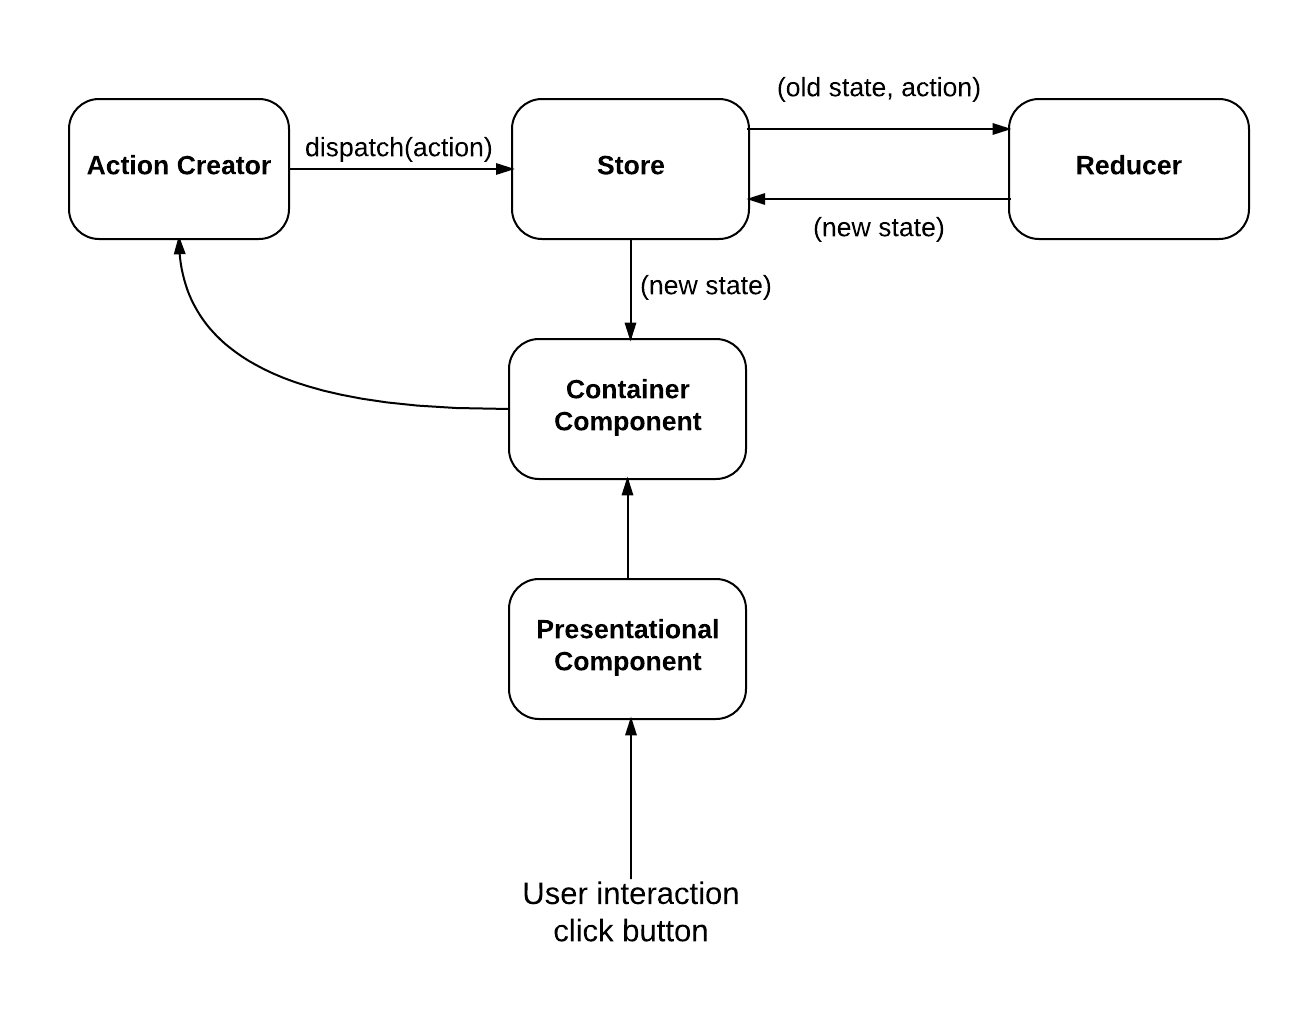
\includegraphics[width=1\textwidth]{assets/redux.png}}
	\caption{Redux structure. Unidirectional dataflow.}	
	\label{fig:redux}
\end{figure}

\subsection{Redux-saga middleware}

The above mentioned Redux flow does not specify where 3d party API calls can be taken care of. It doesn't make much sense to place API calls in container components because then the action dispatching structure will not be utilised. Redux has different middlewares written to take care of that. I chose \verb|redux-sagas| middleware.

Redux-saga is a middleware for taking care of asynchronous actions such as calling 3d party API. Sagas are invoked once at the start of the application and run in the background. Each saga is registered in the store for watching or waiting for a certain action. Once the action is fired saga notices it and performs further logic based on the action. Sagas are created using generator functions. For more information about generator functions please refer to \cite{redux-sagas} chapter External Resources. The generator nature of redux sagas allows writing code in a simple synchronous way. That is a big advantage especially when it comes to API calls and is also easier then creating Promises or using callbacks. Using redux-saga allows to have application logic in two places - reducers which decide on state changes and sagas which take care of data retrieval. \cite{redux-sagas}

The redux-saga midlleware and any other middleware goes in between action creator and the store from the figure  \ref{fig:redux}. Sagas basically catch the action before it reaches the reducers, make some changes and dispatch another action which if not used by any other sagas reaches the reducer.

\subsection{Redux flow example}
Here, I would like to give a simple demonstration of one Redux round for posting a message. The examples are purely for demonstration of the Redux principle. They are inspired by the mobile application implementation but simplified in order not to confuse with extra details. I will describe each snippet and then will summarised the whole process in the end. The following setup is for the application which would serve only one purpose to create messages.

The following is a store registration. \verb|Redux| is imported on line 1, followed by \verb|redux-saga| middleware import. Root reducer is the state changer logic, its example is below.  On line 4 we import a watcher from sagas files and add it to the middleware on line 6. Lines 8 to 16 initialise the store.
\begin{lstlisting}[language=JavaScript]
import { createStore, applyMiddleware } from 'redux'
import createSagaMiddleware from 'redux-saga'
import rootReducer from '../reducers/index.reducer'
import { watchMessagePost } from '../sagas/sagas'

const sagaMiddleware = createSagaMiddleware(watchMessagePost);

export default function configureStore(initialState) {
    return createStore(
        rootReducer,
        initialState,
        applyMiddleware(
            sagaMiddleware
        )
    )
}
\end{lstlisting}

\verb|Index.js| - the entry point of the application. We create the store that was registered in the snippet above here on line 6. The \verb|Provider| import on line 2 enables our application to have access to the store from anywhere. This is very important, since the store holds the application state. You can see that on line 10 the store is passed as the property to the Provider which wraps our CreateContainer.

\begin{lstlisting}[language=JavaScript]
import React, {AppRegistry,Component} from 'react-native';
import { Provider } from 'react-redux'
import configureStore from './app/store/configureStore'
import CreateContainer from './app/containers/create.container'

const store = configureStore();
class AirMsg extends Component {
    render() {
        return (
            <Provider store={store}>
                <CreateContainer />
            </Provider>
        );
    }
}

AppRegistry.registerComponent('AirMsg', () => AirMsg);
\end{lstlisting}

\verb|messages.actions.js| - defines actions and action creators. Each action creator returns a new object. The advised structure of the returned object is as on the following example. It must contain properties type and payload. Each action has its own action creator. 

\begin{lstlisting}[language=JavaScript]
/** Actions */
export const MESSAGE_POST = 'MESSAGE POST';
export const MESSAGE_POST_SUCCESS = 'MESSAGE POST SUCCESS';
export const MESSAGE_POST_FAILURE = 'MESSAGE POST FAILURE';

/** Action creators */
export function postMessage(data) {
    return {
        type: MESSAGE_POST,
        payload: {
            message: data        
        }
    };
}

export function postMessageSuccess(data) {
    return {
        type: MESSAGE_POST_SUCCESS,
        payload: {
            new_message: data
        }
    };
}

export function postMessageFailure(error, action) {
    return {
        type: MESSAGE_POST_FAILURE,
        payload: {
            error: error
        }
    };
}

\end{lstlisting}

\verb|index.reducer.js| can be implemented as a simple switch. It receives state and action in its parameters. The default part of the switch should always return the current state. The initial state is an empty array. Reducer is a place where you could insert some logic which would process action data. 
\begin{lstlisting}[language=JavaScript]
import {
    MESSAGE_POST_SUCCESS,
    MESSAGE_POST_FAILURE
} from "../actions/messages.actions";

const index = (state = [], action) => {
    switch (action.type) {
        case MESSAGE_POST_SUCCESS:
            // place for some processing logic
            return { 
            	new_message: action.payload
				};
        case MESSAGE_POST_FAILURE:
            return action.payload;
        default:
            return state;
    }
};

export default index;
\end{lstlisting}

Part of \verb|sagas.js|. The watcher on line 19 to 21 listens to MESSAGE\_POST action. It will react on every action of this type fired. Once the action is fired the watcher will call postMessage function on line 9. The function will perform the api call on line 11. Thank to the generator nature of sagas we can write code synchronously. Then line 12 dispatches a success action in the case no errors were thrown during the api call. Otherwise the errors are caught and the failure action is dispatched on line 14.

\begin{lstlisting}[language=JavaScript]
import {takeEvery} from "redux-saga";
import {put, call} from "redux-saga/effects";
import {MESSAGE_POST} from "../actions/messages.actions";

var api = require('../api');
var messageActions = require('../actions/messages.actions');

/** workers */
function* postMessage(data) {
    try {
        const resp = yield call(api.post, data.payload);
        yield put(messageActions.postMessageSuccess(resp));
    } catch (error) {
        yield put(messageActions.postMessageFailure(error));
    }
}

/** watchers */
export function* watchMessagePost() {
    yield* takeEvery(MESSAGE_POST, postMessage);
}
\end{lstlisting}

\verb|create.container.js| is a container which renders a \verb|createComponent| on line 10. It is connected to the store and has full access to the state. The function which maps the state to container properties is on line 19. Another function mapping functions that dispatch actions to the store is on line 25. And finally on line 31 both of these functions are connected with our container. On line 27 I map postMessage action from \verb|messages.actions.js| to the container properties. On the line 21 i make part of the state available to my container to access through its properties. Once I call function from line 27 the POST\_MESSAGE action will be dispatched to the store. On line 13 this function is passed as a property to the Component, keeping the logic on the side of containers and providing component with a callback to react on user interaction.

\begin{lstlisting}[language=JavaScript]
var React = require('react-native');
import {connect} from "react-redux";
import {bindActionCreators} from "redux";
import * as messageActions from "../actions/messages.actions";

var CreateComponent = require('../createComponent');

class CreateMsgContainer extends React.Component {

    render() {
        return ( 
        		<CreateComponent 
        			postMessage={(m) => this.props.postM(m)} 
						/>
				);
    }
}

const mapStateToProps = (store) => {
    return {
			message: store.new_message    
    };
};

const mapDispatchToProps = (dispatch) => {
    return {
        postM: bindActionCreators(messageActions.postMessage, dispatch)
    };
};

CreateMsgContainer = connect(mapStateToProps, mapDispatchToProps)(CreateMsgContainer);
module.exports = CreateMsgContainer;
\end{lstlisting}

There is no example of component since it is just a simple form with a button, the button would have onclick event set to the function passed to it in properties.

Now I would like to sum up all of the above snippets in order to form a whole picture. The application starts and \verb|index.js| is called. It initializes the store with initial state null and creates the application, passes the store to the application through properties and renders the \verb|create.container.js|. Container render function renders \verb|createComponent| which has a form for user interaction. User submits a message. The \verb|onClick| event fires (it was passed from the container through properties). The event fires POST\_MESSAGE action. The saga watcher is waiting for that action. It grabs the action and passes it to its worker. The worker calls api to save the message. If everything goes ok and the returned response status is 200 the POST\_MESSAGE\_SUCCESS action is fired. The reducer receives the action and changes the state according to implementation. By changing the state the reducer forces re-render of container and component. Container has state store.new\_message mapped to its properties. Now once the whole cycle is finished the container can do something with the received data. 

\subsection{Augmented Reality}
As I have previously stated in chapter Analysis and design section \nameref{section:ar} I chose Wikitude SDK for implementation of Augmented Reality in the mobile application. 

Wikitude SDK has a plugin for IOS development with Javascript API which I decided to use. There is no direct support for React Native, but the plugin provides a developer with Wikitude framework and there is a set of instructions how to integrate AR in the native iOS application on their website (for reference see official setup guide \cite{wikitude}). 

\subsubsection{Connecting React Native and Objective C}
React Native is a set of javascript functions wrapped around native code. Therefore you can make your application communicate with the native code using Native Modules or Native UI Components. This is particularly useful when you want to implement part of you application's functionality natively.  

There are two macros which one can use:  \verb|RCT_METHOD_EXPORT(*method*)| and \verb|RCT_MODULE_EXPORT()|. Further is described the one that I used.

\begin{itemize}
\item  \verb|RCT_MODULE_EXPORT()| 
This macro says that the given class is exported to React Native and can be referenced by its name. It is considered to be good programming style to separate your files into header (\verb|.h| extension) and implementation files (\verb|.m| extension). For an example of exporting a module see the following classes below: \verb|ExampleManager.h|, \verb|ExampleManager.m| and \verb|Component.js|.


\begin{lstlisting}[language=C]
// ExampleManager.h
#import "RCTViewManager.h"

@interface ExampleManager : RCTViewManager
@end

\end{lstlisting}

\begin{lstlisting}[language=C]
// ExampleManager.m
#import <YourCustomView.h>

#import "RCTViewManager.h"
#import "ExampleManager.h"

@implementation ExampleManager

RCT_EXPORT_MODULE()

- (UIView *)view
{
  return [[YourCustomView alloc] init];
}

@end
\end{lstlisting}

\begin{lstlisting}[language=javascript]
// Component.js
import {React, requireNativeComponent} from 'react-native';

var Example = requireNativeComponent('Example', Component);

class Component extends React.Component {
  render() {
    return <Example />;
  }
}

module.exports = Component;
\end{lstlisting}
  
  \verb|ExampleManager.h| is a header file and it solely defines the interface and possible attributes or parameters for the main class. For our purposes it extends RCTViewManager who takes care of views in React Native, hence the suffix RCT.
  
  \verb|ExampleManager.m| implements \verb|view| function which returns \verb|UIView*| on line 11. This function is called by default on any class representing a view in Objective C, when it is mounted in the view hierarchy.
  
  \verb|Component.js| is the actual component we use in our React Native application. In order to use Native UI Component which we defined in  \verb|ExampleManager.h| and \verb|ExampleManager.m| we add an import on line 2 and require native component on line 4. After that the native view is ready to use as a simple react component as you can see on line 8.
  

\end{itemize}
\subsubsection{Object format}

The supported format for 3d files by Wikitude is \textit{wt3}, which is their own 3d format. For now there is no support for programatic conversion which I could have implemented in my web application. This bring a certain overhead. However wikitude provides their own converter which converts \textit{fbx} file to \textit{wt3}. It is free and available at wikitude website \cite{wikitude}. 


\subsubsection{Integration of Wikitude and RN}
To start using Wikitude SDK you first need to add it to our XCode project and create a ViewController as described in the official setup guide at \cite{wikitude}. There is also a sample project available at \cite{wiki-project} that shows an example of ViewController implementation. For my purposes I had to modify the sample implementation. The complete implementation for integration of Wikitude and React Native is found in Appendix: \nameref{apendix:integration}. 

However this implementation works while testing in simulator and with cable attached, it crashes the application once tested on device not connected with the cable. After thorough research I found out that React Native core mounts each view twice for styling reasons \cite{RNcode}.
This creates a memory leak because the ArchitectWorld object in the application is allocated twice, which is an unwanted behaviour for the Wikitude. The simulator only throws warning and is not affected by the memory leak. On the contrary when the application is tested on device and the Augmented Reality is launched it crashes the application, shutting it down with no chance of continuing using it. I didn't come accross that issue sooner because my initial research didn't show any signs of incompatibility of React Native and Wikitude. Furthermore I didn't find any example of their integration so I simply thought due to the young age of React Native that it hasn't been tried out before.

To conclude Wikitude is not entirely suitable for using with React Native at the moment. However I believe with growing popularity of React Native there will be a plugin released for it soon. Once the plugin is out I could change the Augmented Reality logic part of the application and replace it with the plugin.

\subsection{Libraries used}


I have used npm package manager for taking care of the dependencies in the project. Among all the libraries I have used there are a few I would like to mention.

\begin{itemize}
	\item react-native-image-picker 
	
	This React Native module allows access to the phone's photo gallery and the camera. Also it sends the photo taken to the camera back to javascript in base64 format. \cite{image-picker} \item react-native-autocomplete 
	
	Neat module, wrapping around native autocomplete module. It shows a dropdown of suggested autocomplete matches as user types. It is also highly configurable, from styles to the actual funciton \textit{onTyping()}. It provides callback on every event fired by the native module. \cite{autocomplete}
	
	\item react-native-maps 
	
	The official facebook documentation for React Native offers this map as a better alternative to their own map implementation. This library offers different map manipulations such as controlling map events, tracking location, programatically changing region, using animated API and many others. \cite{maps}
\end{itemize}


\section{Web Application}

Web application is implemented using React and Redux, which has been already described in detail in the previous section \nameref{redux-section}.


\subsection{Functionality}

The main functionality is access through the menu sections: 3D gallery, My Gallery, Upload 3D and Statistics.

\begin{itemize}
\item 3D Gallery

Web application allows user to browse through a common object gallery to choose 3d objects. Each object can be added to user's gallery.

\item Upload 3D 

The user can upload his own 3D images in the request format following the guidelines next to the upload form.

\item My Gallery

In this part the user can see which object were added to his gallery.

\item Statistics

The user can view statics for TOP 10 messaging country and city by accessing Statics in the menu. Furthermore the user can see statistics on his messages. How many times each message has been viewed and how many comments was left on each message, when was the last comment.
\end{itemize}

Screenshots of each part of the web application are found in the appendix.
\subsection{Routing}

I used \verb|redux-router| \cite{react-router} for handling the routing in the web application. It is a routing library for the React which allows to create user friendly, pretty urls without hashes and use browser history.  Since React is view only framework the navigation is purely on the client side and all the routes work only if you start navigating from the index route. Basically you have to have the application loaded and then you are able to move around changing routes. When your route is missing the hash, which is usually present in javascript application routes, the request is sent to the server. Once you refresh any of the pages which is not the index page the route will not be found since there is no such route on the server unless you specifically created it. Therefore for React routing to function properly there is a need for a server. There are several options of how to accomplish that. 

Firstly there is server side rendering option. The server will be serving complete html pages with data and everything needed. In the case of high load and data heavy websites it is a very good choice since it brings high performance and is also SEO friendly. However Google seems to be enhancing their indexing and crawling mechanisms in order to be able to crawl through javascript pages \cite{google-blog}. 

Secondly a simple server which will serve as a proxy can be created. This option seemed more suitable for me. The web application is pretty basic so the performance increase from moving to server rendering will not be that essential. For the meantime for the purposes of my web application server with a proxy is enough.

I implemented a simple express server which on all incoming requests redirects to index.html allowing the application to load and serve the user requested route. The example of the express server can be found in Appendix \ref{apx:react-server}

\subsection{Libraries used}

Here are a few of the most helpful libraries I came across while working on the web application.

\begin{itemize}
	
	\item react-bootstrap 
	
	Famous Bootsrap library wrapped with React Components. As the original Bootstrap library allows easy styling. \cite{react-boot}
	\item react-masonry-component
	
	Neat masonry library, which allows easy organizing of objects on the gird.  \cite{react-masonry}
	\item react-d3 
	
	D3 chart utilities enabled for React. The library supports various types of charts, for instance: line chart, scatter chart, bar chart and area chart. \cite{react-d3}
	
\end{itemize}
\section{Testing}


\subsection{Unit tests}
Unit testing is a type of automated testing focused on testing functionality of separate units of system in isolation. Targets of unit testing could be functions, React components and classes. Unit tests are tests closest to the code itself, they do not test any business logic but pure functionality. To make sure the tested code is isolated a developer mocks subcomponents and services used by the class/component he is testing. \cite{redux-tests} Unit tests help during development. If they are frequently written the developer can make bold changes to the code and easily check whether any of the previous functionality is broken by simply running the tests. Tests should be maintained and changed with the growing code base to make sure they have a solid code coverage.

\subsubsection{Framework}

When looking for a testing framework my main concern was to find one framework I could easily use for all the technologies involved in my project. I needed a framework with support for testing node, easily calling API endpoints, traversing React tree, accessing React's components, and being able to parse, and deal with React Native components.

There is a plethora of javascript testing frameworks. However, not that many of them support or have a smooth way of working with React or React Native. The main issue with React Native is that it does not render html but native components. Therefore, each component needs to be mocked separately. While some like \verb|Text| are easy to mock others like \verb|Animate| leave you puzzled. Therefore, a big part of testing React Native is mocking which should not be the focus of the testing process. The developer needs to focus on the tests, not on mocks. Until recently the best way to test React and React Native was \verb|Jest| \cite{jest}. It is a very good choice for testing since it mocks everything automatically and the developer can focus on writing tests rather than creating mocks for components. I tried Jest. However, I was dissatisfied with its speed and after reading about possible other issues that might arise such as mocking everything, event the libraries you do not want to have mocked, I decided to look for another solution. \cite{redux-tests}

The next testing framework I tried was Mocha \cite{mocha}. Mocha is not created for testing React but there are complimentary libraries which help with that. For instance \verb|enzyme| \cite{enzyme} was designed specifically for this purpose. \verb|Enzyme| is a javascript testing utility which allows traversing React DOM, assert and manipulate with React's components with ease. Moreover, recently \verb|react-native-mock| \cite{react-native-mock} came out, which is a mocker for all the React Native components written by Leland Richardson. Combining \verb|react-native-mock|,  \verb|mocha| and \verb|enzyme| provides a powerful setup with easy and elegant testing process.

\subsubsection{Execution}

Before running unit tests first of all make sure all the dev dependencies are installed. Test dependencies are included for the development environment only. That saves time when installing the project and disk space.

\lstdefinestyle{nonumbers}
{numbers=none}

\begin{lstlisting}[language=C, style=nonumbers]
 npm install --only=dev
\end{lstlisting}

To run unit tests in any of my applications simply run the following in the command line.

\begin{lstlisting}[language=C, style=nonumbers]
npm test
\end{lstlisting}

\subsection{Redux testing}

Unit testing on its own is not enough to test the mobile and web applications. It is also important to test the data flow system I am using - Redux.
Redux tests can be broken down into several categories: 
\begin{itemize}
	\item Action Tests
	
	These tests will make sure the action creators return the correct actions upon being called.
	\item Reducer Tests
	
	These test take care of verifying the correct transition between states. The test checks if the reducer returns the correct state upon receiving dispatched action.
	\item Middleware Tests
	
	The middleware in Redux flow is responsible for catching the dispatched action before it reaches reducer, performing some logic and then dispatching another action based on result of the performed logic. These tests are very important for both web and mobile applications since they are testing communication and data retrieval.
\end{itemize}

Redux testing will be performed using \verb|mocha|, \verb|enzyme| and \verb|react-native-mock|.

\subsubsection{Execution}

These tests are run the same way as the unit tests.

\setsecnumdepth{part}
\chapter{Conclusion}

The main task of using only Javascript technologies for creating a messaging system with mobile application, web application and a server was accomplished. Both non functional requirements and functional requirements have been fulfilled. The system is highly performant due to the chosen technologies: \verb|node.js|, \verb|React| and \verb|React Native|. It would easily recover in case of a crash.  External processes such as \verb|supervisor| make sure the server and the queue consumers are restarted in case of failure. The server API is well documented with documentation easily accessible from the index page. Moreover, the system is scalable and is ready for high request load. Load balancer is configured to serve that purpose. In case of the server overloading it only takes a minute to add a new server to load balancer's configuration to scale the system. The system is easily extendable due to the nature of chosen implementation technologies.

It must be also mentioned that Javascript is a very powerful technology, which is underestimated by many. It is flexible and has a lively community with many contributors. React has already transformed the way web front-end is made. React Native, an amazing creation of Facebook engineers, is definitely worth while and has a big future ahead of it. It revolutionises the way mobile applications are created and gives access to mobile development to wider audience. And last but not the least is \verb|node.js| which makes writting server side code pleasant.

To conclude I would like to say that I am very happy for having an opportunity to explore these amazing technologies and to have a chance to create a solid, highly functional system using them.




\bibliographystyle{iso690}
\bibliography{bibliography/bibliography}

\setsecnumdepth{all}
\appendix

\chapter{Acronyms}
% \printglossaries
\begin{description}
	\item[AR] Augmented Reality	
	\item[DOM] Extensible markup language	
	\item[JS] Javascript	
	\item[MB] Megabyte	
	\item[POI] Point of Interest
	\item[SDK] Software Development Kit	
	\item[SQL] Structured Query Language				
	\item[3D] Three dimensional		
	
\end{description}

\chapter{Installation guide}

\section{Server}

\subsection{Dependencies}
\begin{itemize}
  \item Npm
 \item Redis
  \item MongoDb
  \item Supervisor 
  \item Nginx
\end{itemize}

\noindent
Start installing dependencies by running the following command.
\begin{lstlisting}[language=C, style=nonumbers]
 npm install
\end{lstlisting}

\noindent
The rest of dependecies are available for download at their official websites.
Configuration files for \verb|Supervisor| and \verb|Nginx| are provided in folder \verb|configuration| on the enclosed CD.

\subsection{Execution}
\noindent Start the Redis server.
	\begin{lstlisting}[language=C, style=nonumbers]
	 redis-server
	\end{lstlisting}
	
\noindent Start the MongoDb in the server directory. It will be using directory data, in case u want mongo to use another directory, just specify it as the command argument.
	\begin{lstlisting}[language=C, style=nonumbers]
	 mongod --dbpath=data
	\end{lstlisting}	
	
\noindent Now you configure supervisor, by adding both consumers and a server in the configuration. Run supervisor and specify the configuration file path. You can either configure your commands to run at the start or run the command line utility \verb|supervisorctl| and start them from there. If you used provided supervisor config the commands will run on start.
	\begin{lstlisting}[language=C, style=nonumbers]
	 supervisord --configuration=FILE
	\end{lstlisting}	
		
\noindent The server is ready to take requests now. It is running on \url{http://localhost:3000}


\section{Mobile application}

\subsection{Dependencies}
\begin{itemize}
  \item XCode
  \item Npm
  \item Rnpm
\end{itemize}
\subsection{Execution}

Install XCode from the official website or through the AppStore.
\\~\\
\noindent
Start installing dependencies by running the following command.
\begin{lstlisting}[language=C, style=nonumbers]
 npm install
\end{lstlisting} 

\\~\\
\noindent Link the external dependencies to the Objective C project in XCode.
\begin{lstlisting}[language=C, style=nonumbers]
 rnpm link
\end{lstlisting} 

\\~\\
\noindent Open \verb|AppDelegate.m| from the \verb|ios| folder and make sure there is a correct address set for the \textit{jsCodeLocation}.

\\~\\
\noindent There is a folder \verb|/app/config| which has configuration for the server address. Set the correct address of the server in there.

\\~\\
\noindent Compile the project. You can either run it on the in-built simulator or on a connected device.


\section{Web application}

\subsection{Dependencies}
\begin{itemize}
  \item Npm
\end{itemize}

\subsection{Execution}
\noindent
Start installing dependencies by running the following command.
\begin{lstlisting}[language=C, style=nonumbers]
 npm install
\end{lstlisting}

\\~\\
\noindent The web application needs to have a server started to run. In folder \verb|server| in the web application implementation run the following command.
\begin{lstlisting}[language=C, style=nonumbers]
 npm run
\end{lstlisting}
\noindent An express server is ready to take requests now. 

\noindent In your browser navigate to \url{http://localhost:3001}. You should be able to interact with the web application now.

\\~\\
\noindent There is a folder \verb|/app/config| which has configuration for the server address. In case the web and the server will not be running on the same machine that configuration will have to be replaced with the actual server address.

\chapter{Mobile application screenshots}

\begin{figure}[!ht]
	\centering
	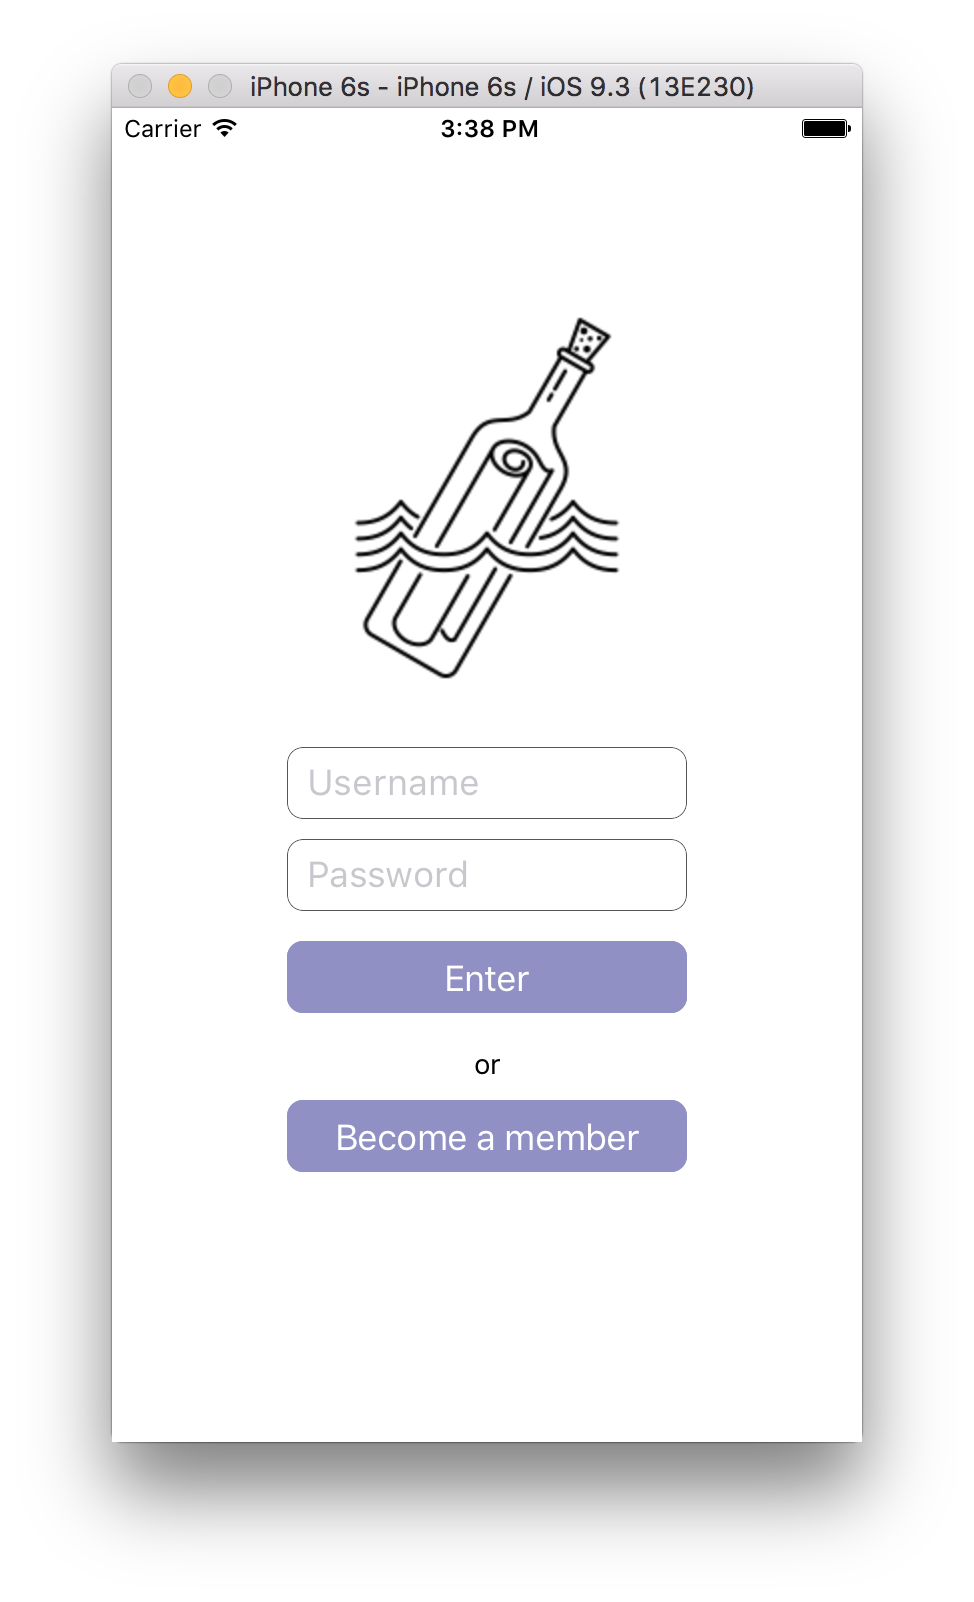
\includegraphics[width=0.6\textwidth]{assets/mobile_screens/login.png}}
	\caption{Mobile application. Login}
\end{figure}


\begin{figure}[!ht]
	\centering
	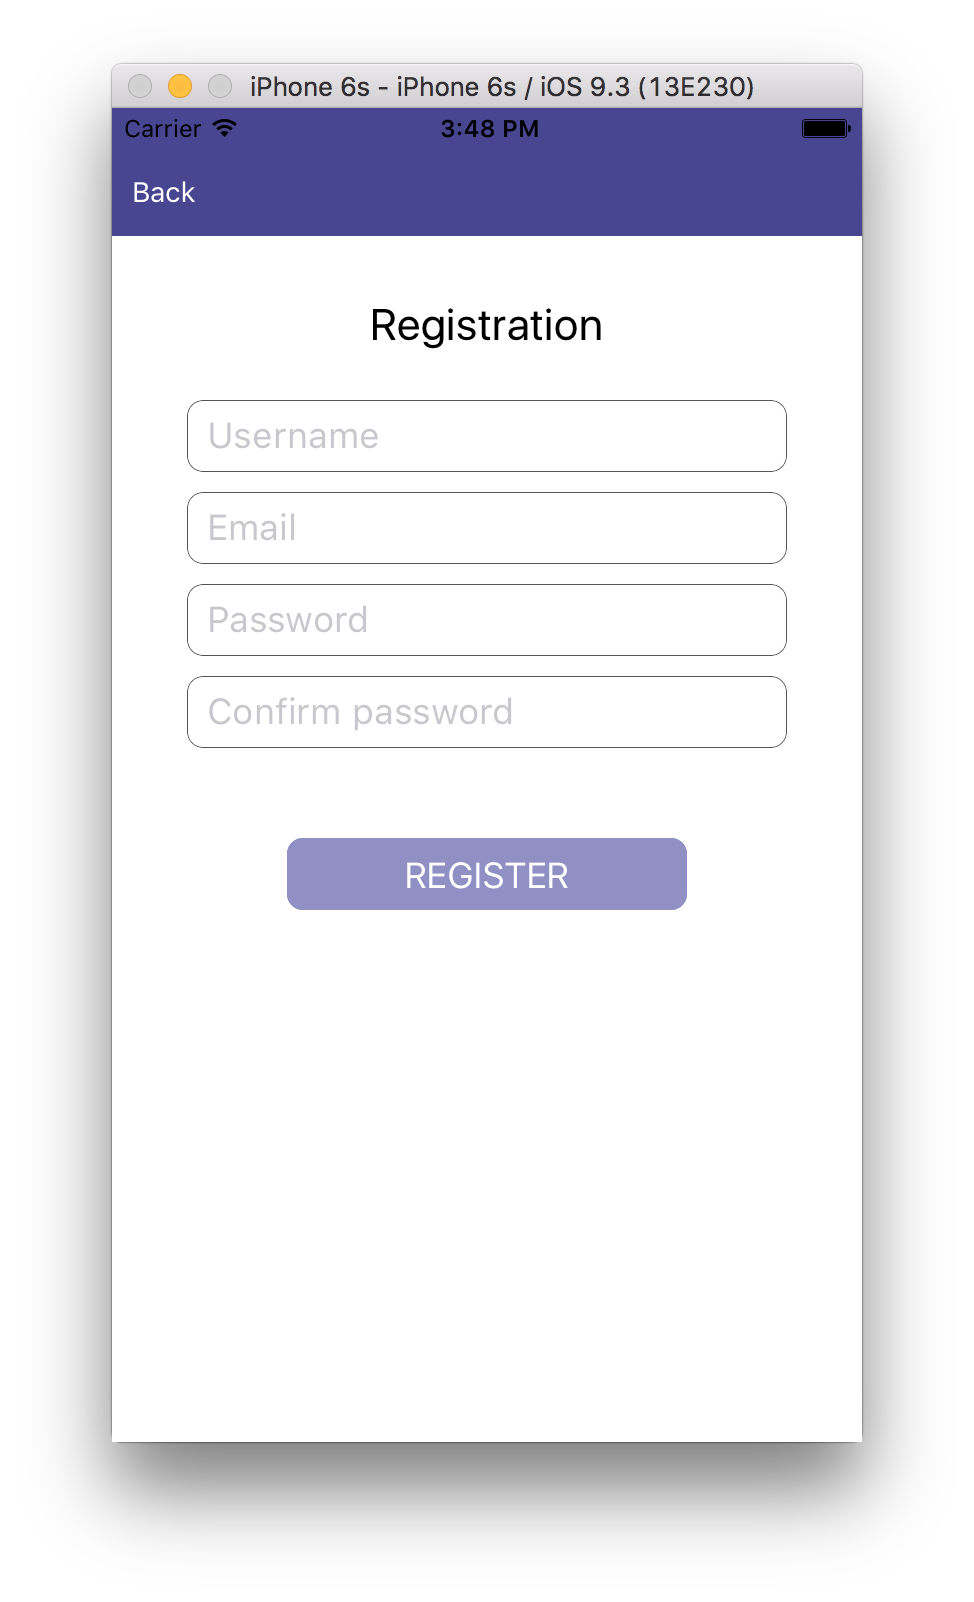
\includegraphics[width=0.8\textwidth]{assets/mobile_screens/register.png}}
	\caption{Mobile application. Registration}
\end{figure}

\begin{figure}[!ht]
	\centering
	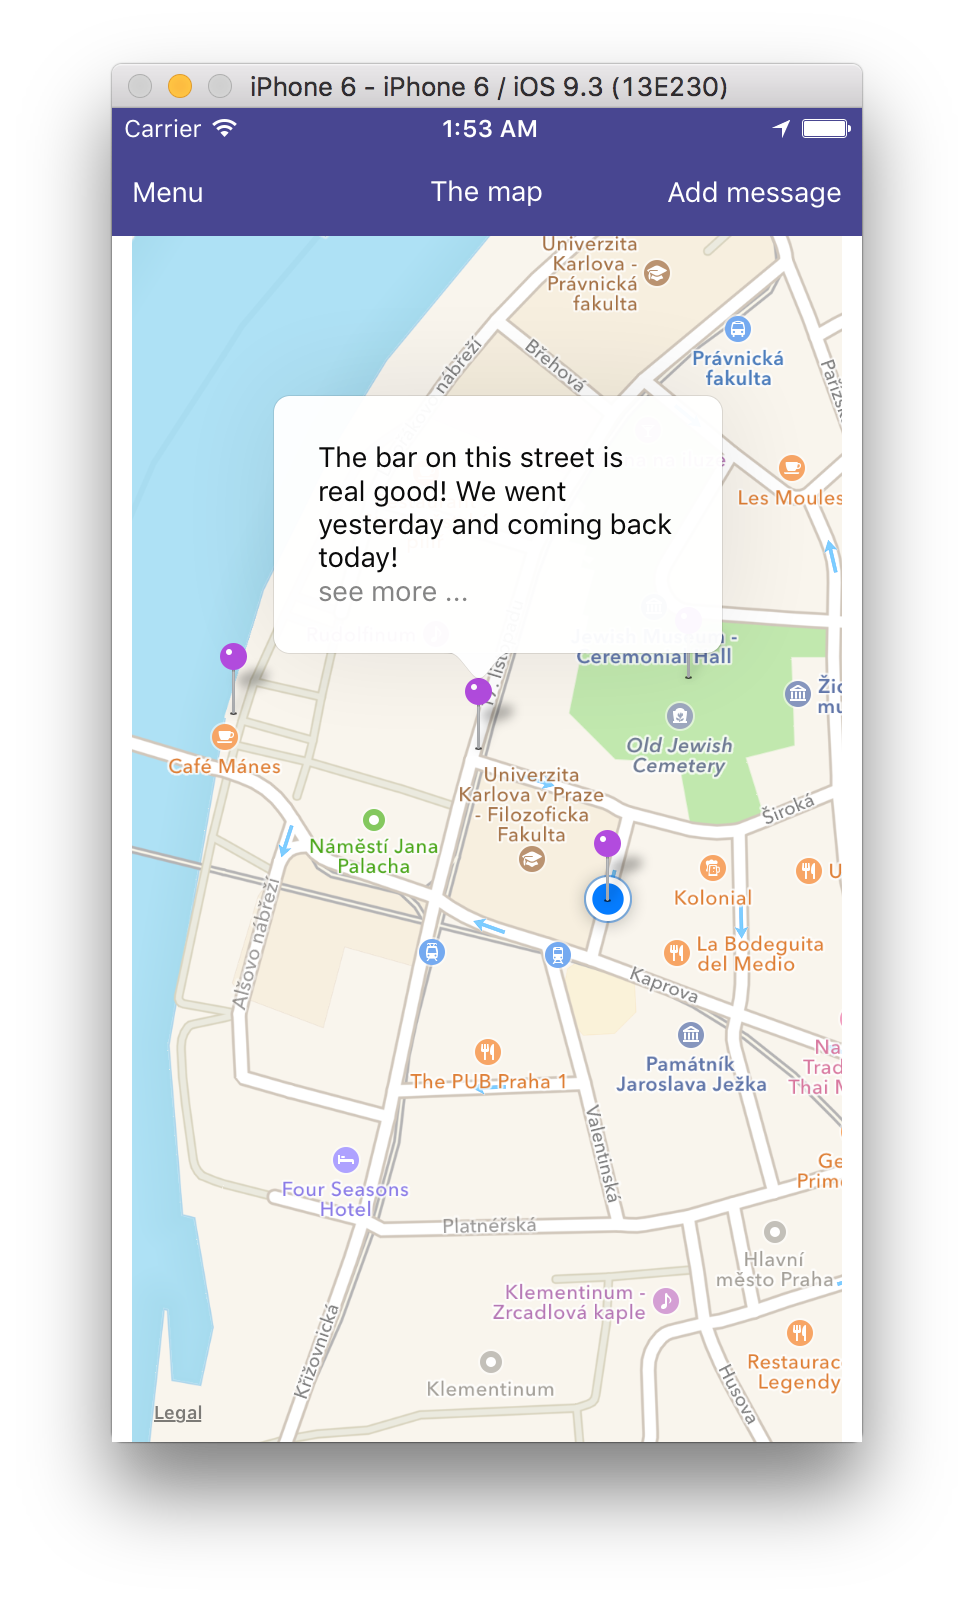
\includegraphics[width=0.8\textwidth]{assets/mobile_screens/map.png}}
	\caption{Mobile application. Messages map}
\end{figure}


\begin{figure}[!ht]
	\centering
	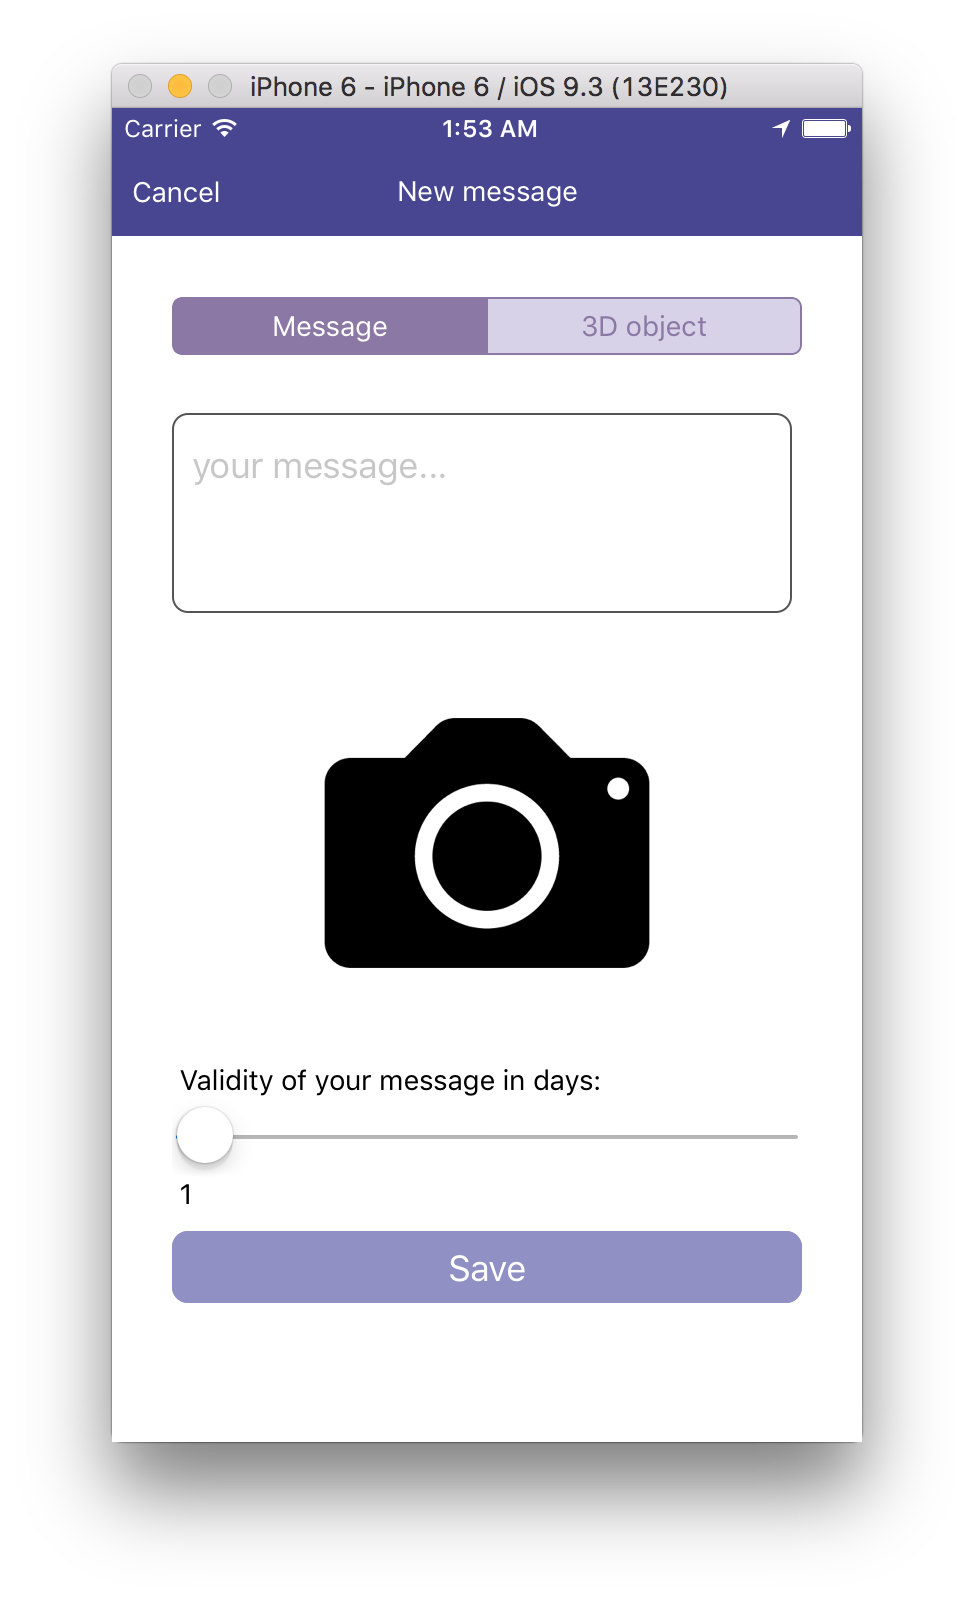
\includegraphics[width=0.8\textwidth]{assets/mobile_screens/add_text_message.png}}
	\caption{Mobile application. Adding a text message}
\end{figure}

\begin{figure}[!ht]
	\centering
	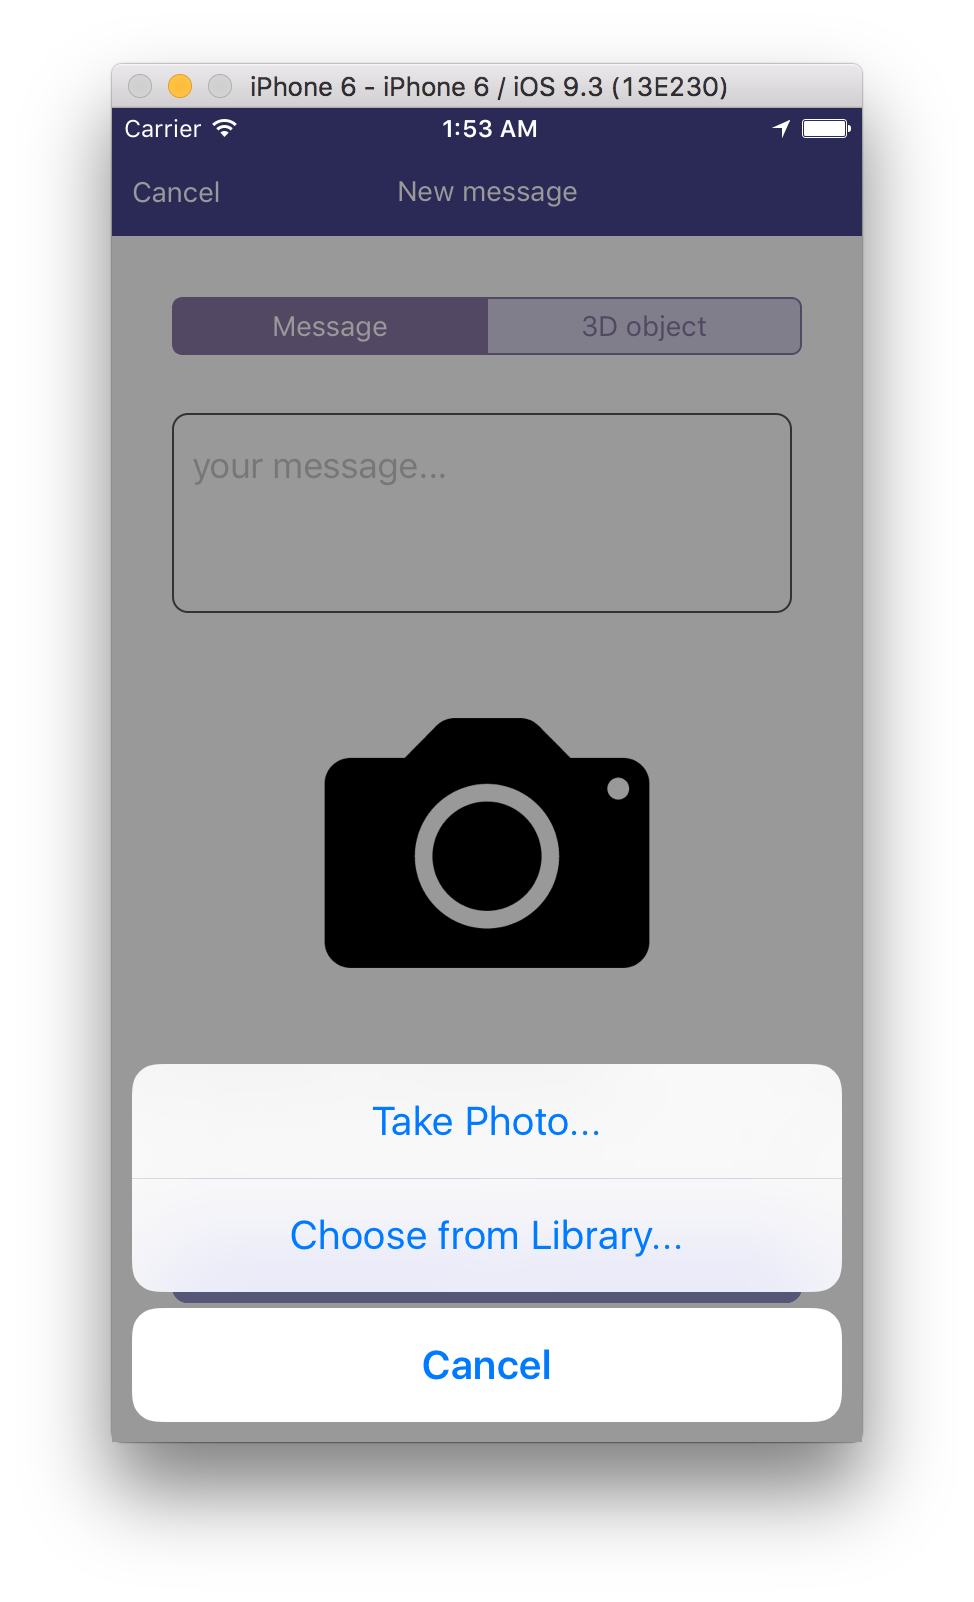
\includegraphics[width=0.8\textwidth]{assets/mobile_screens/adding_image.png}}
	\caption{Mobile application. Adding image to text message}
\end{figure}


\begin{figure}[!ht]
	\centering
	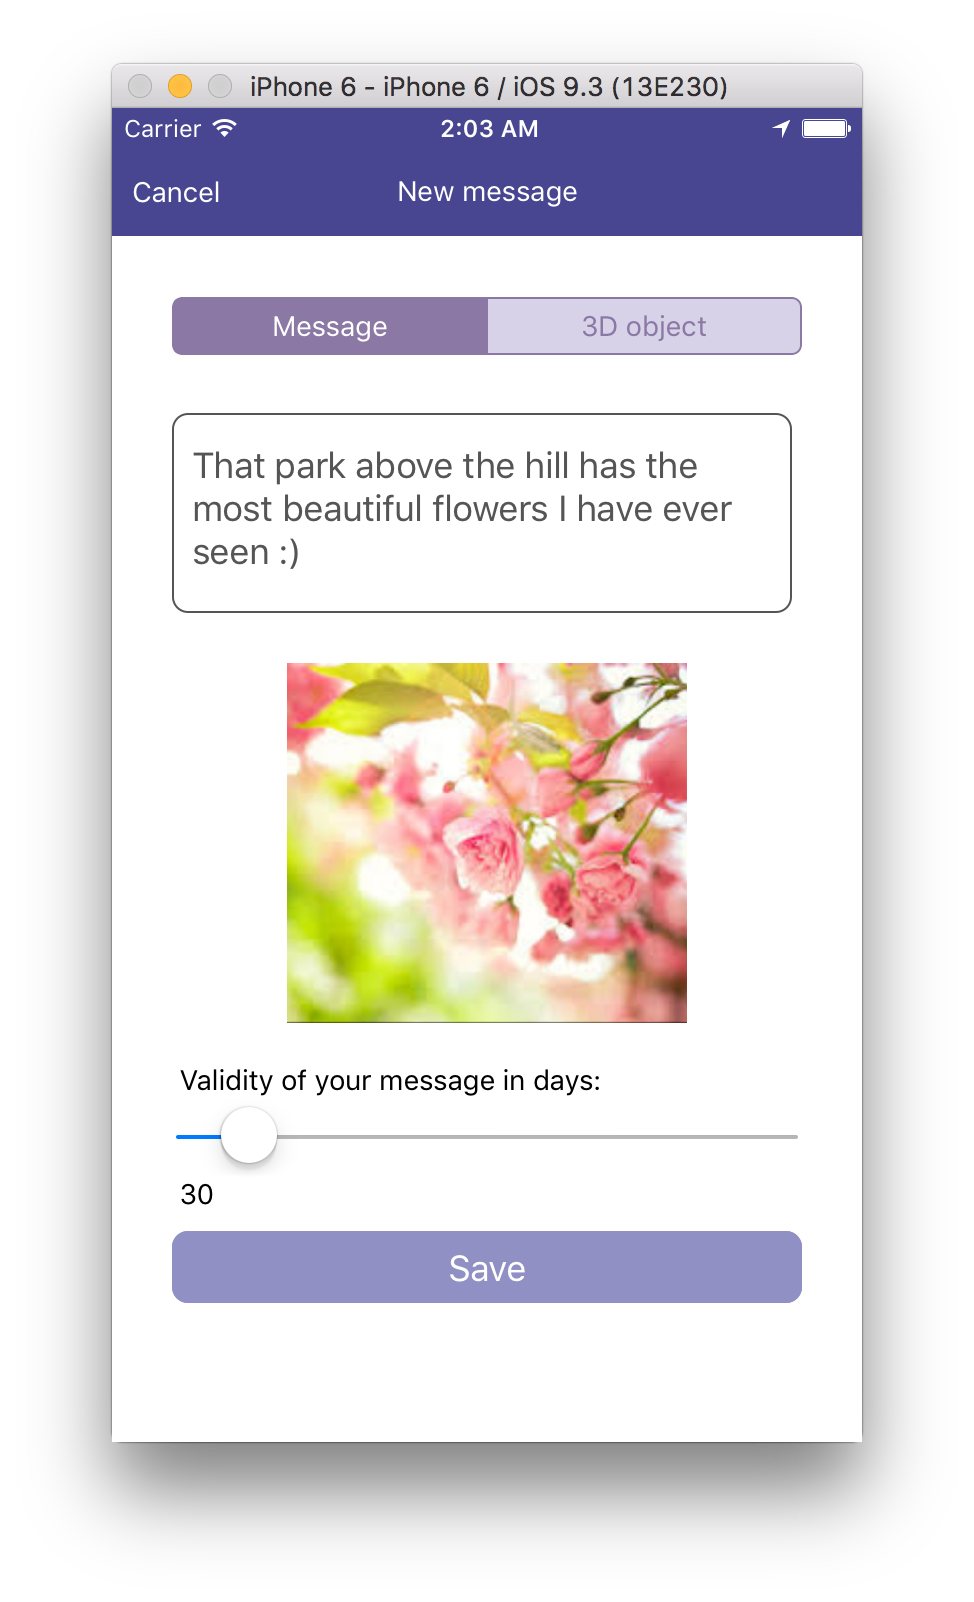
\includegraphics[width=0.8\textwidth]{assets/mobile_screens/message_with_image.png}}
	\caption{Mobile application. Message with image and text}
\end{figure}


\begin{figure}[!ht]
	\centering
	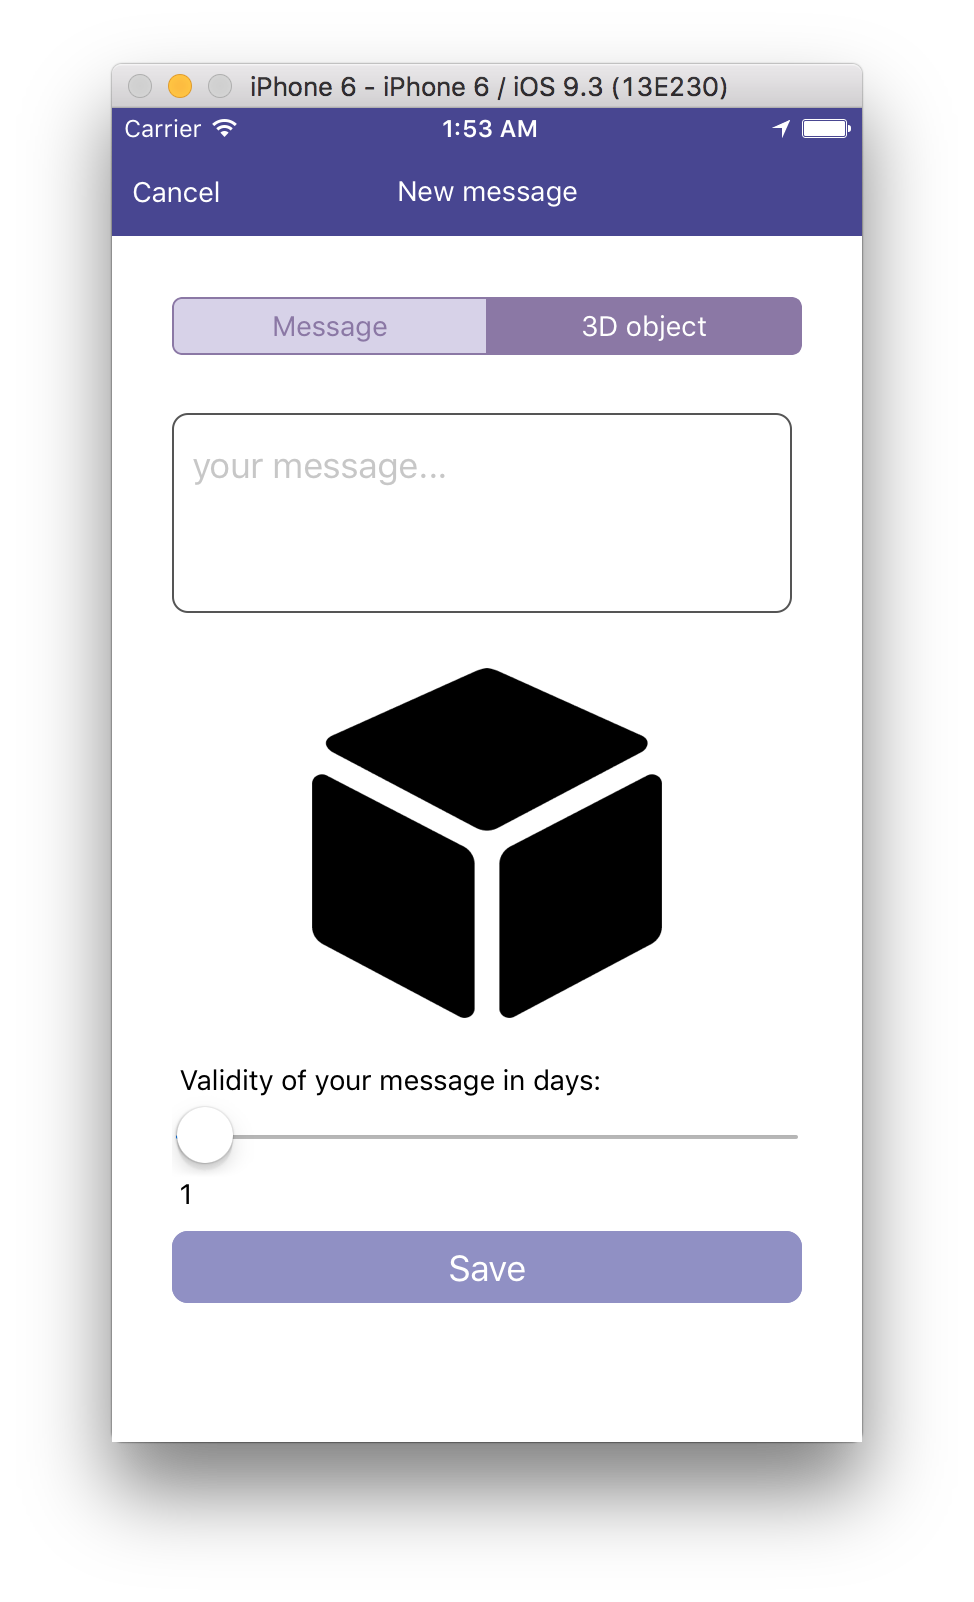
\includegraphics[width=0.8\textwidth]{assets/mobile_screens/3d_message.png}}
	\caption{Mobile application. 3D Message option chosen}
\end{figure}


\begin{figure}[!ht]
	\centering
	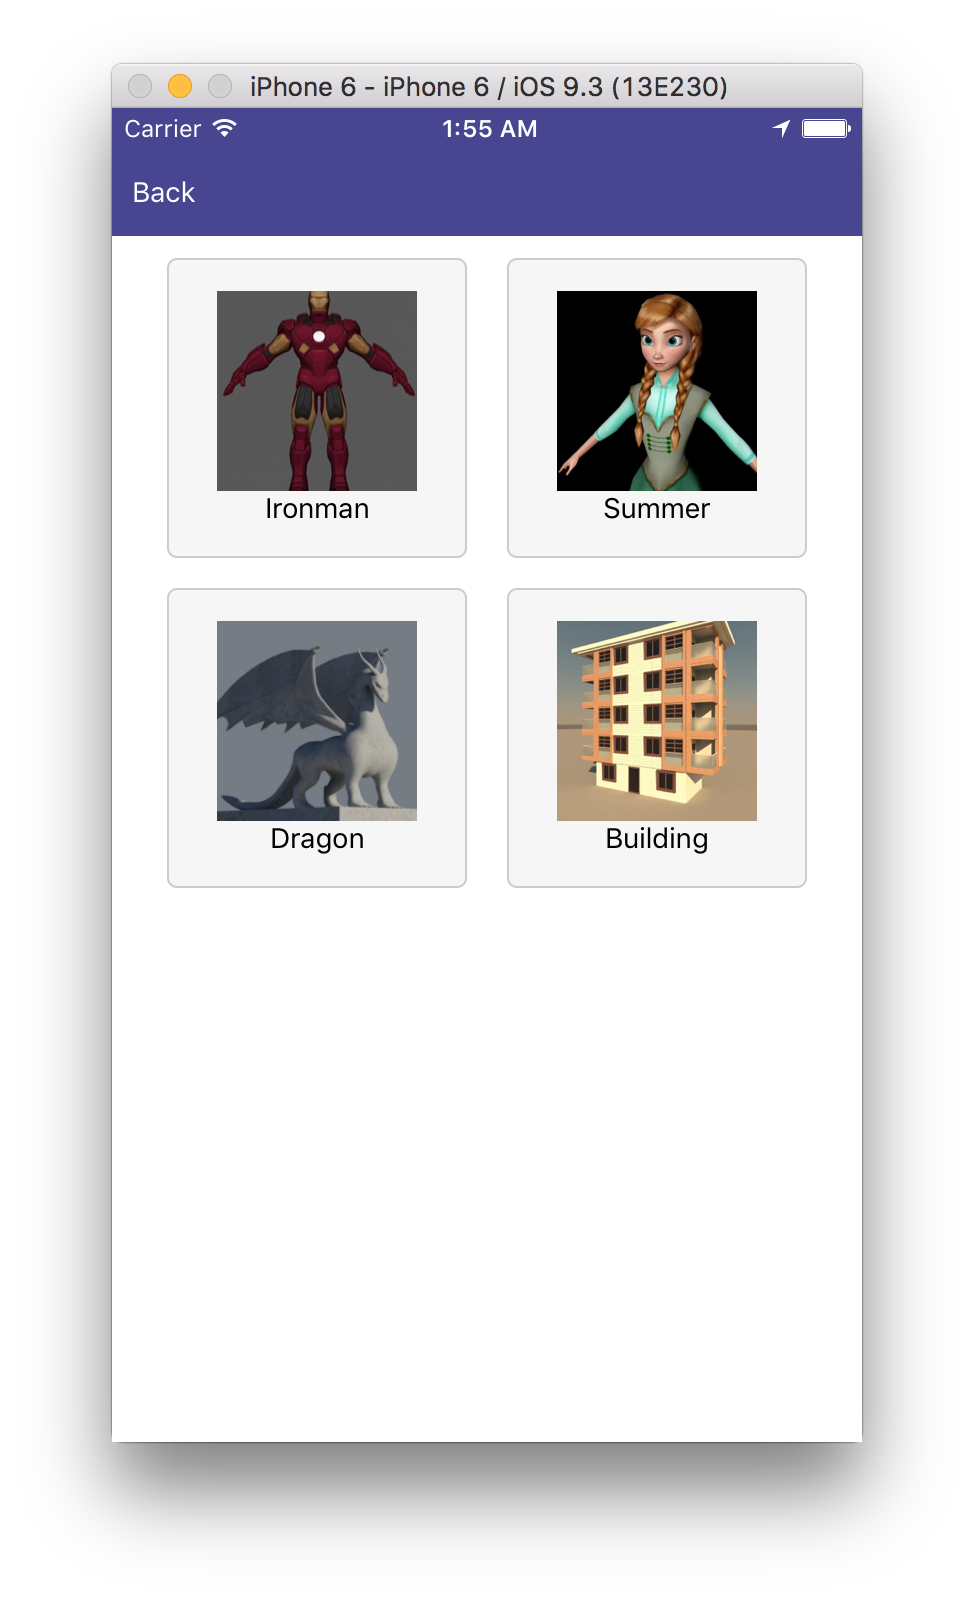
\includegraphics[width=0.8\textwidth]{assets/mobile_screens/object_gallery.png}}
	\caption{Mobile application. User's object gallery. It is accessible when attaching an object to the message.}
\end{figure}


\begin{figure}[!ht]
	\centering
	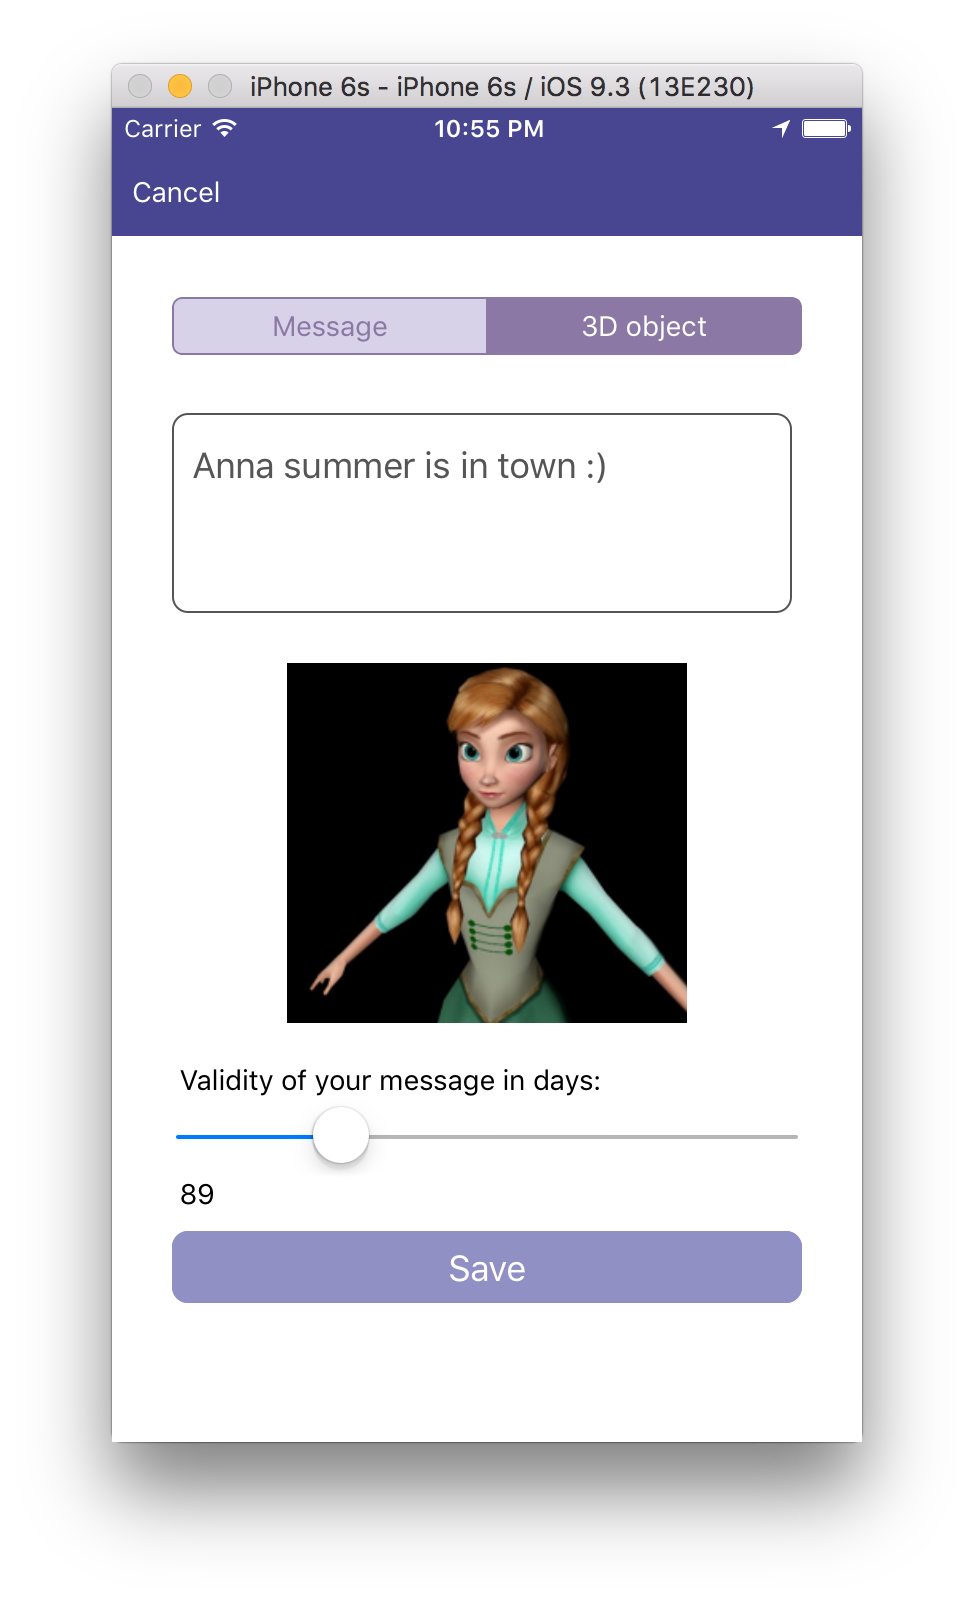
\includegraphics[width=0.8\textwidth]{assets/mobile_screens/3d_message_view.png}}
	\caption{Mobile application. 3D Message thumbnail preview}
\end{figure}


\begin{figure}[!ht]
	\centering
	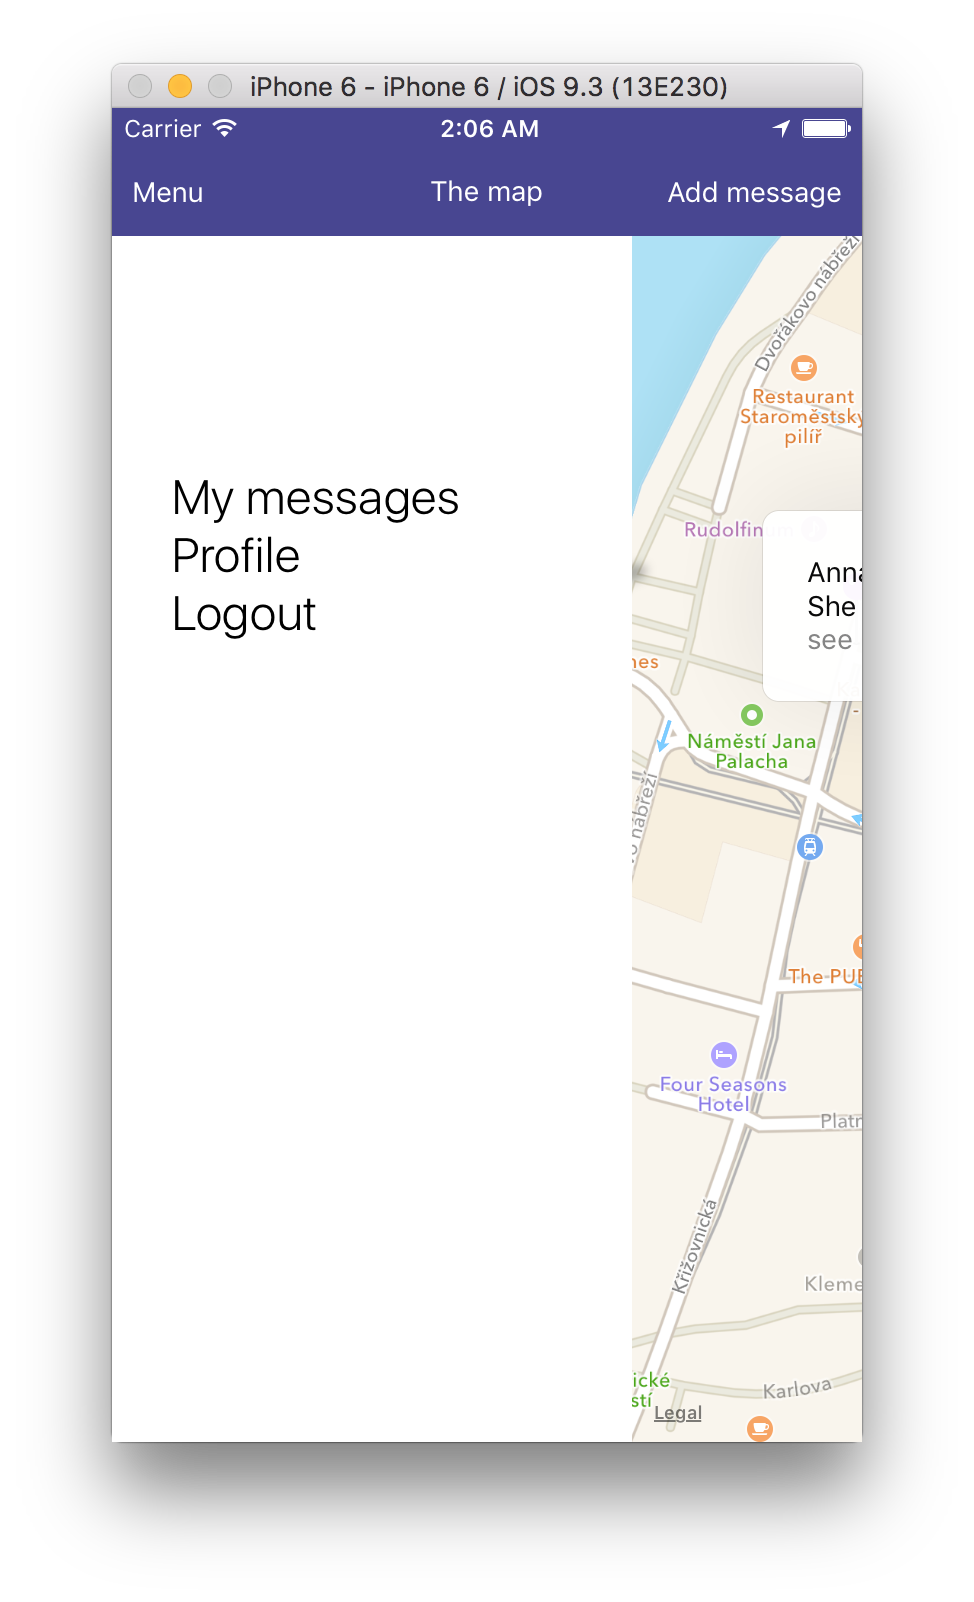
\includegraphics[width=0.8\textwidth]{assets/mobile_screens/menu.png}}
	\caption{Mobile application. Menu}
\end{figure}


\begin{figure}[!ht]
	\centering
	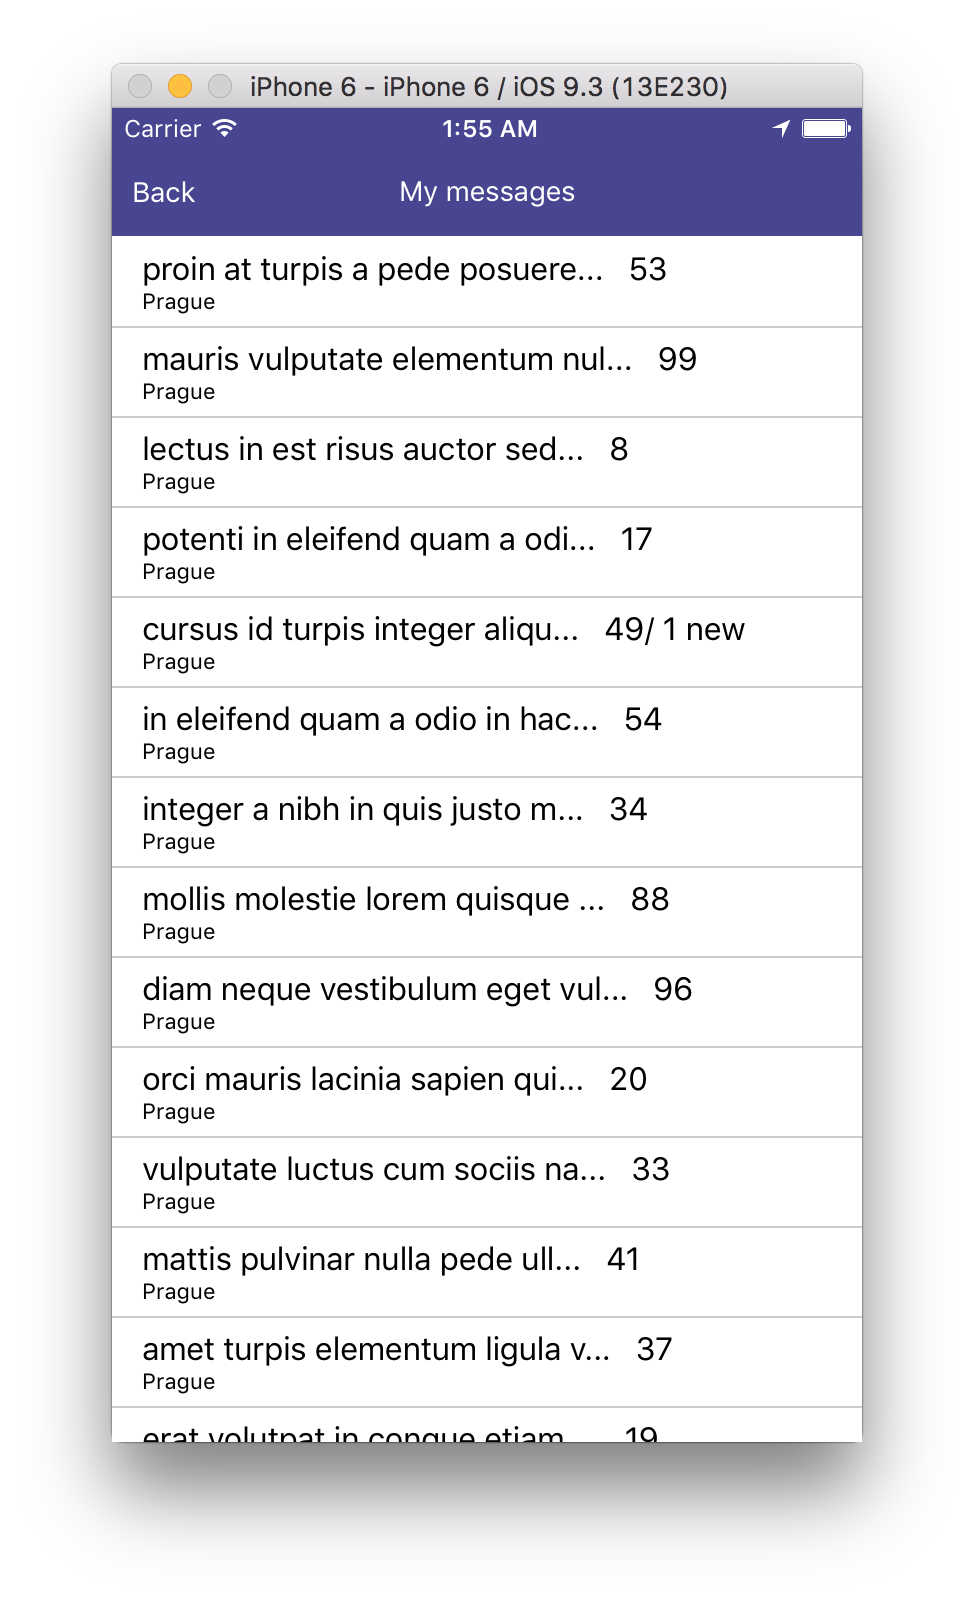
\includegraphics[width=0.8\textwidth]{assets/mobile_screens/my_messages.png}}
	\caption{Mobile application. My messages}
\end{figure}



\begin{figure}[!ht]
	\centering
	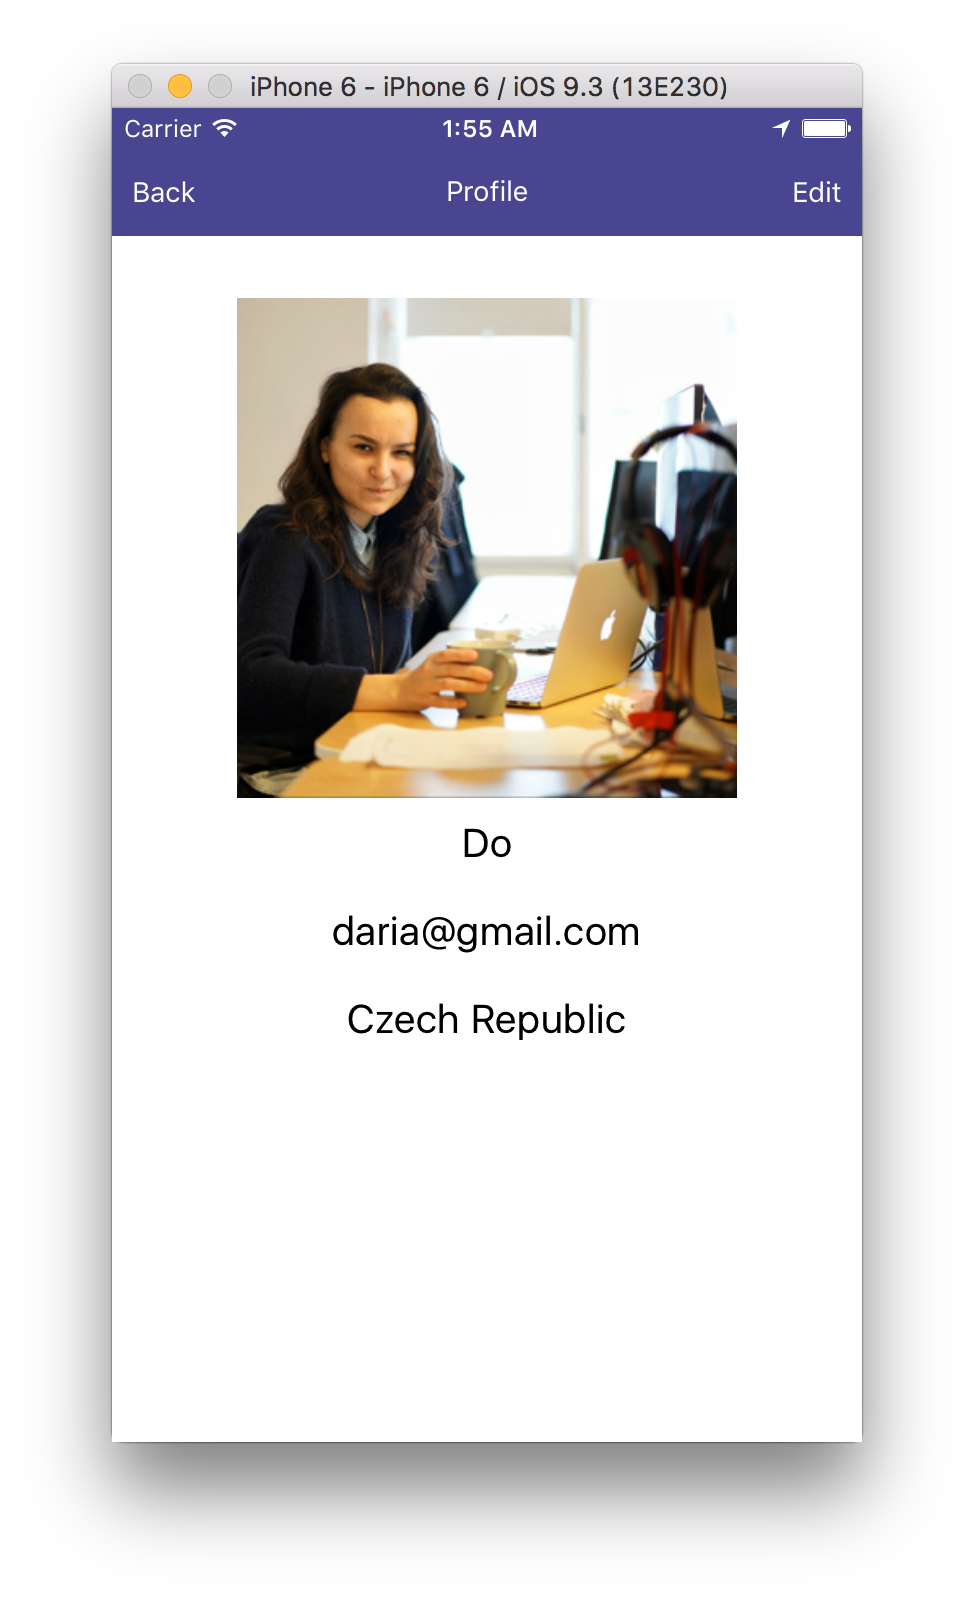
\includegraphics[width=0.8\textwidth]{assets/mobile_screens/profile.png}}
	\caption{Mobile application. Profile}
\end{figure}


\begin{figure}[!ht]
	\centering
	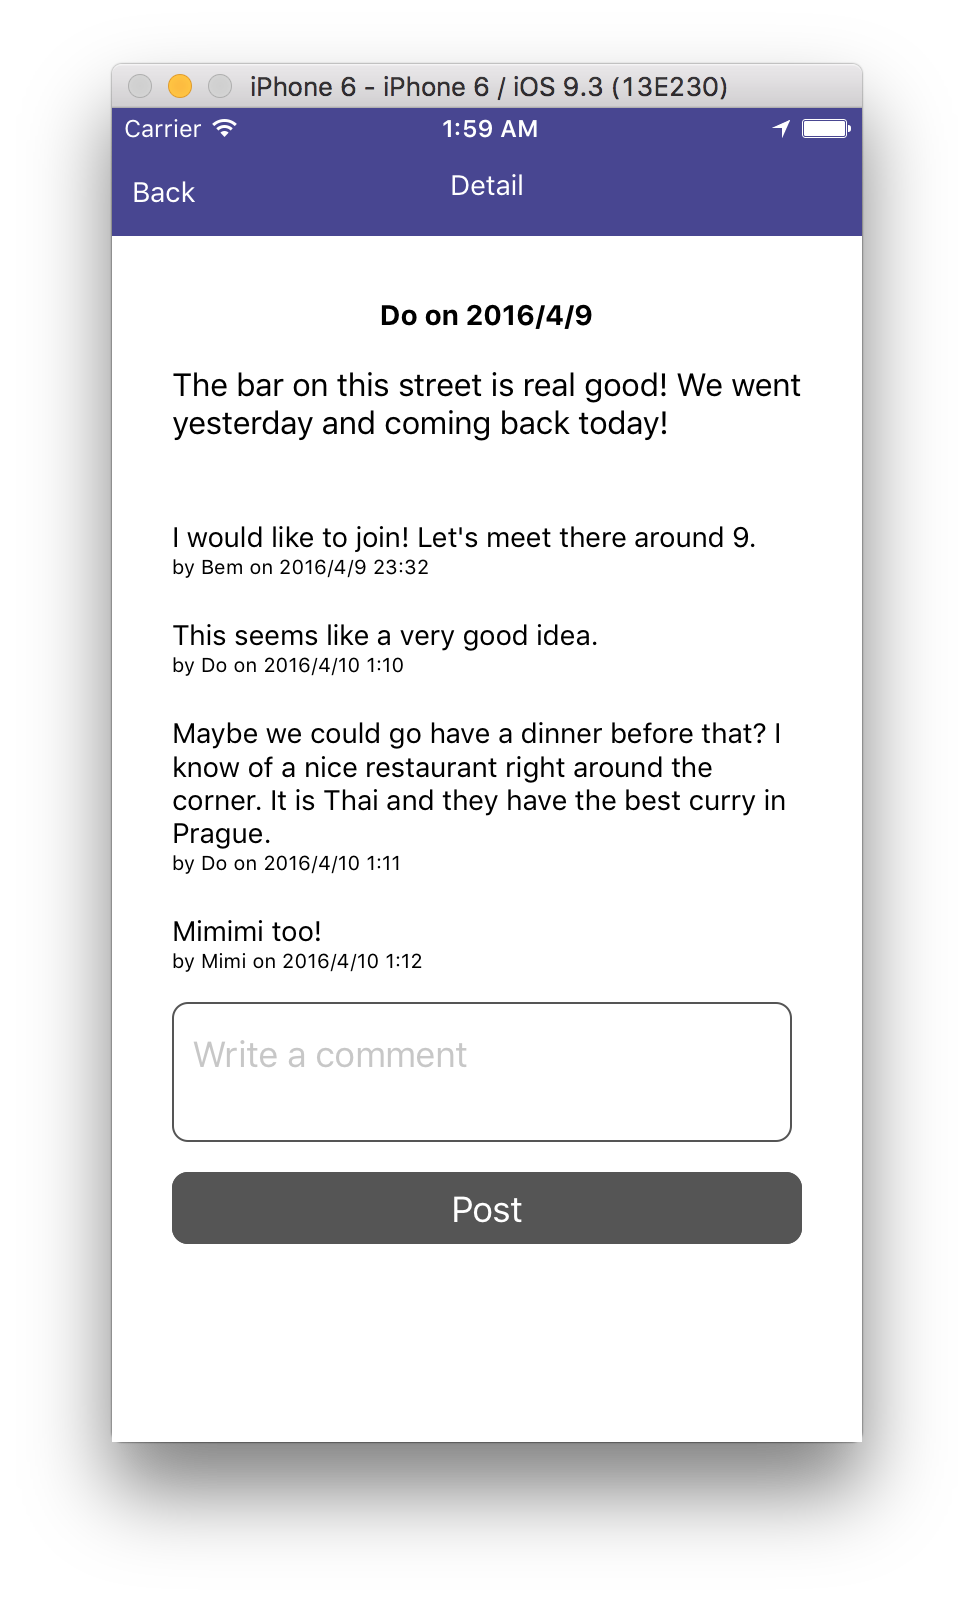
\includegraphics[width=0.8\textwidth]{assets/mobile_screens/detail.png}}
	\caption{Mobile application. Message detail}
\end{figure}



\begin{figure}[!ht]
	\centering
	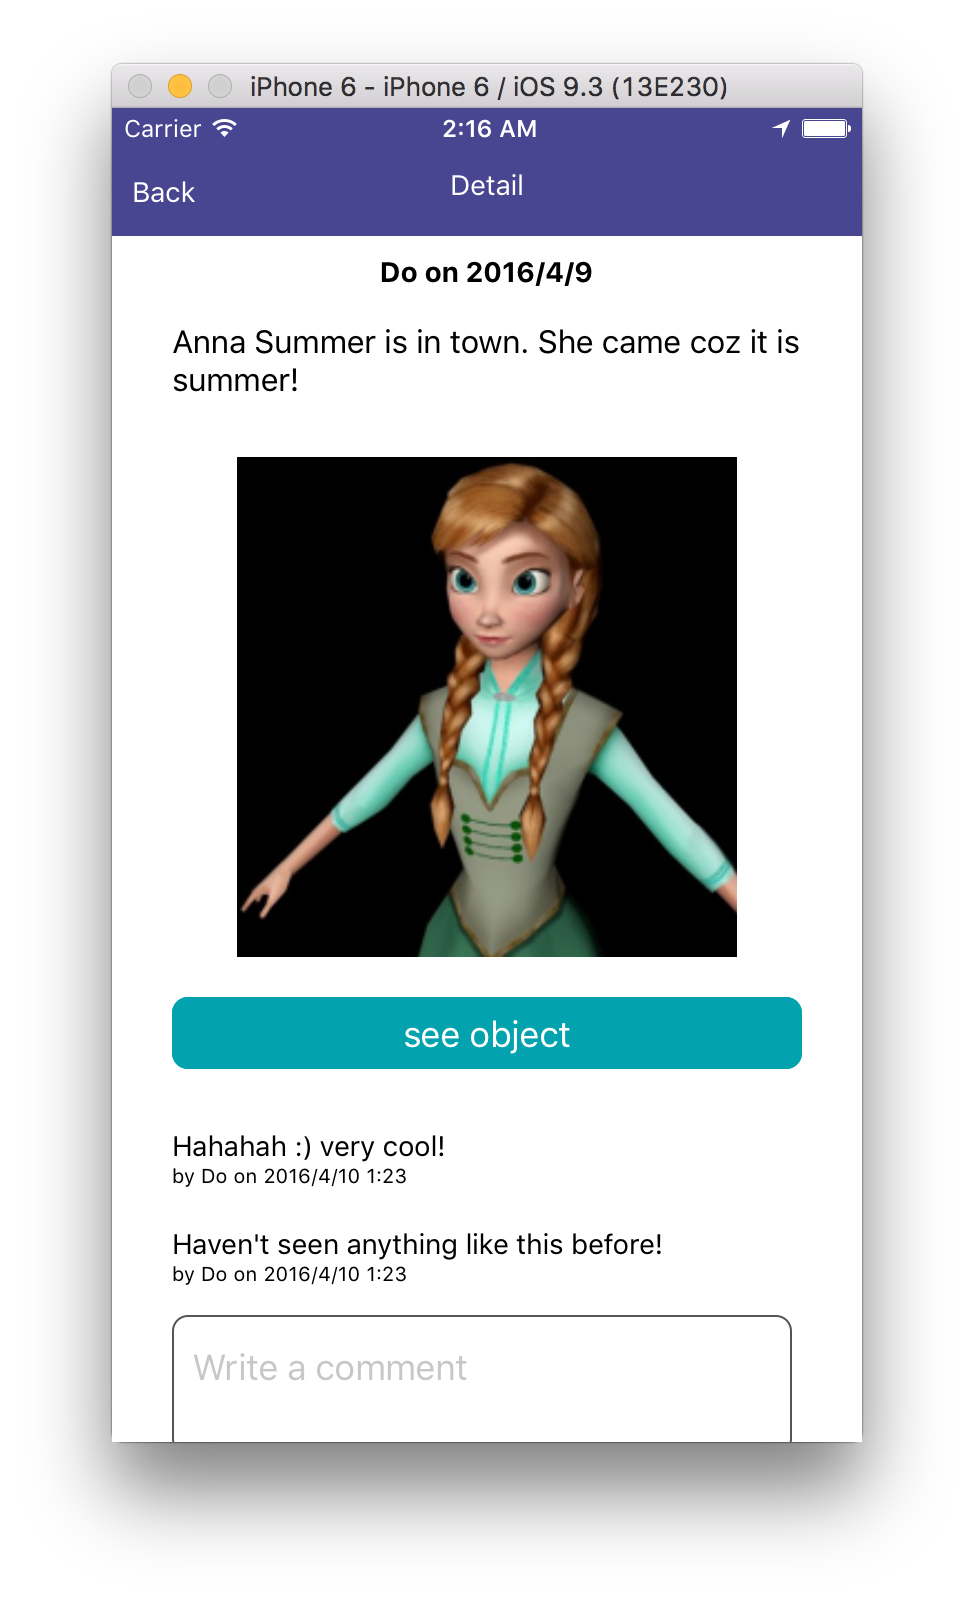
\includegraphics[width=0.8\textwidth]{assets/mobile_screens/3d_detail.png}}
	\caption{Mobile application. 3D Message detail. Augmented Reality starts when "see object" button is tapped.}
\end{figure}





\chapter{Web application screens}

Web application is made as a complimentary portal mainly to allow user to choose 3d objects from the common gallery, add these obejcts to his gallery or upload his own 3d objects, see information about his messages and view statistics by country and city.

\begin{figure}[!ht]
	\centering
	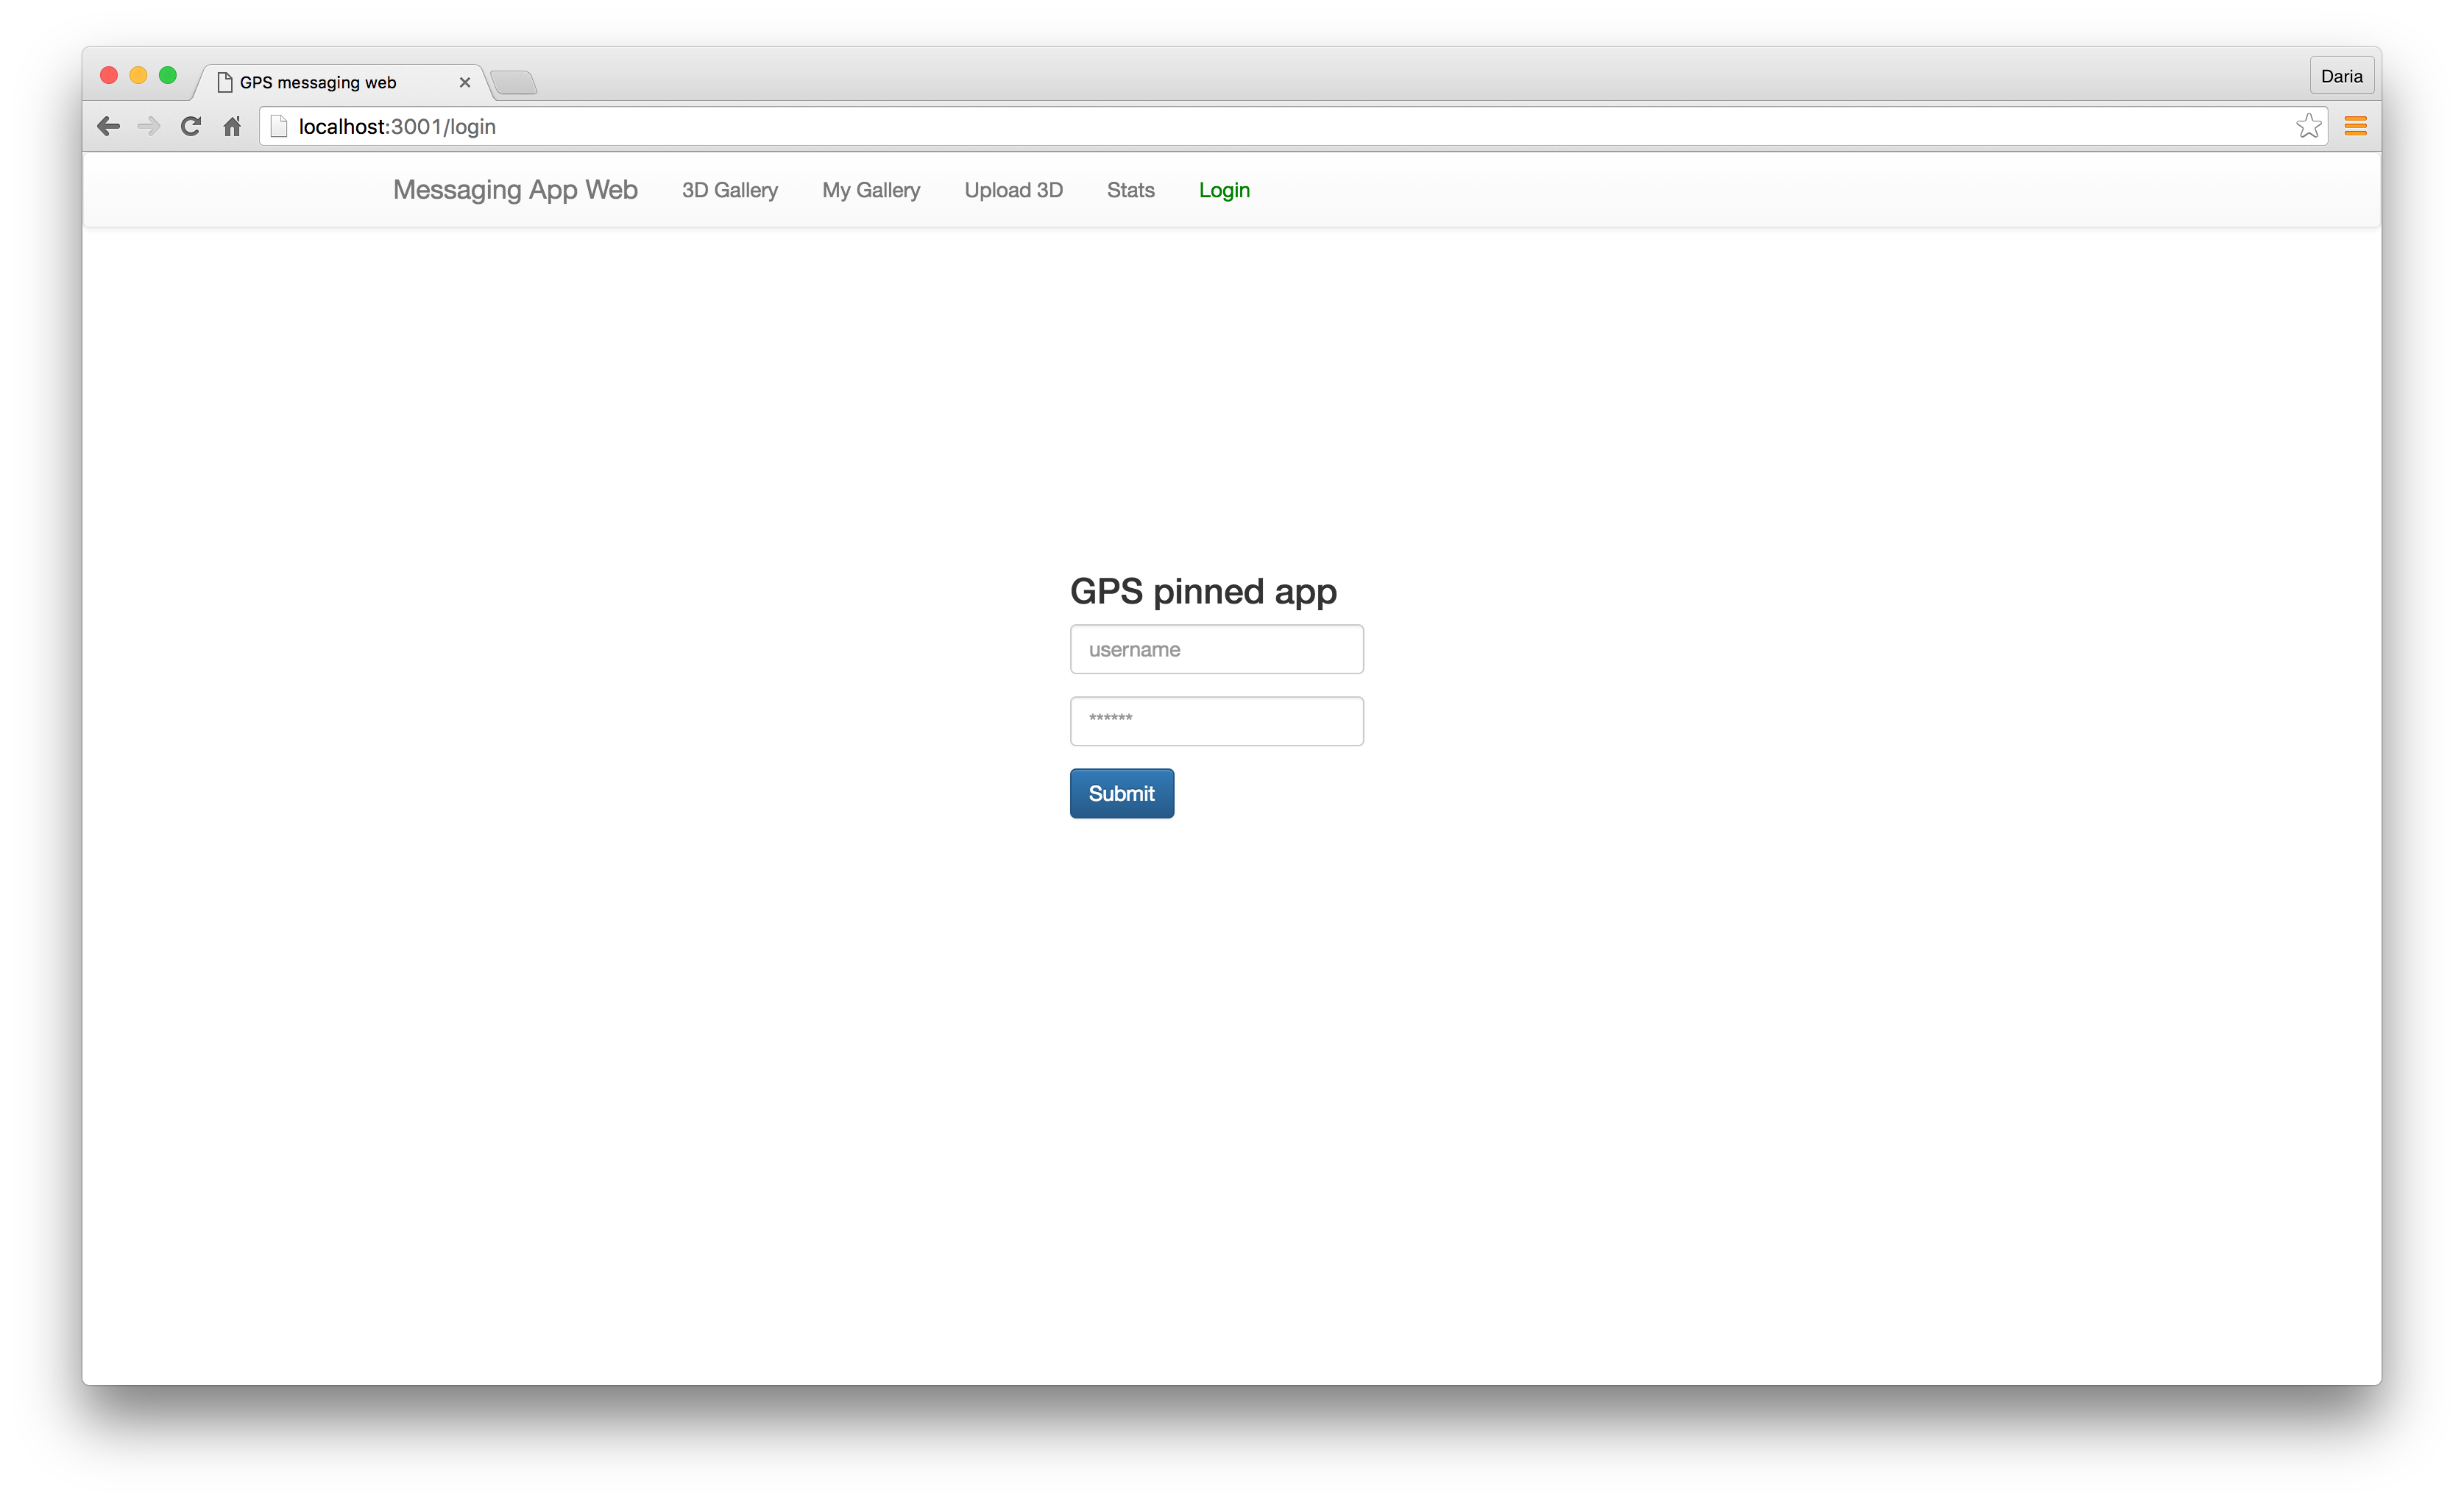
\includegraphics[width=0.8\textwidth]{assets/web_screens/login.png}}
	\caption{Web application. Login}
\end{figure}

\begin{figure}[!ht]
	\centering
	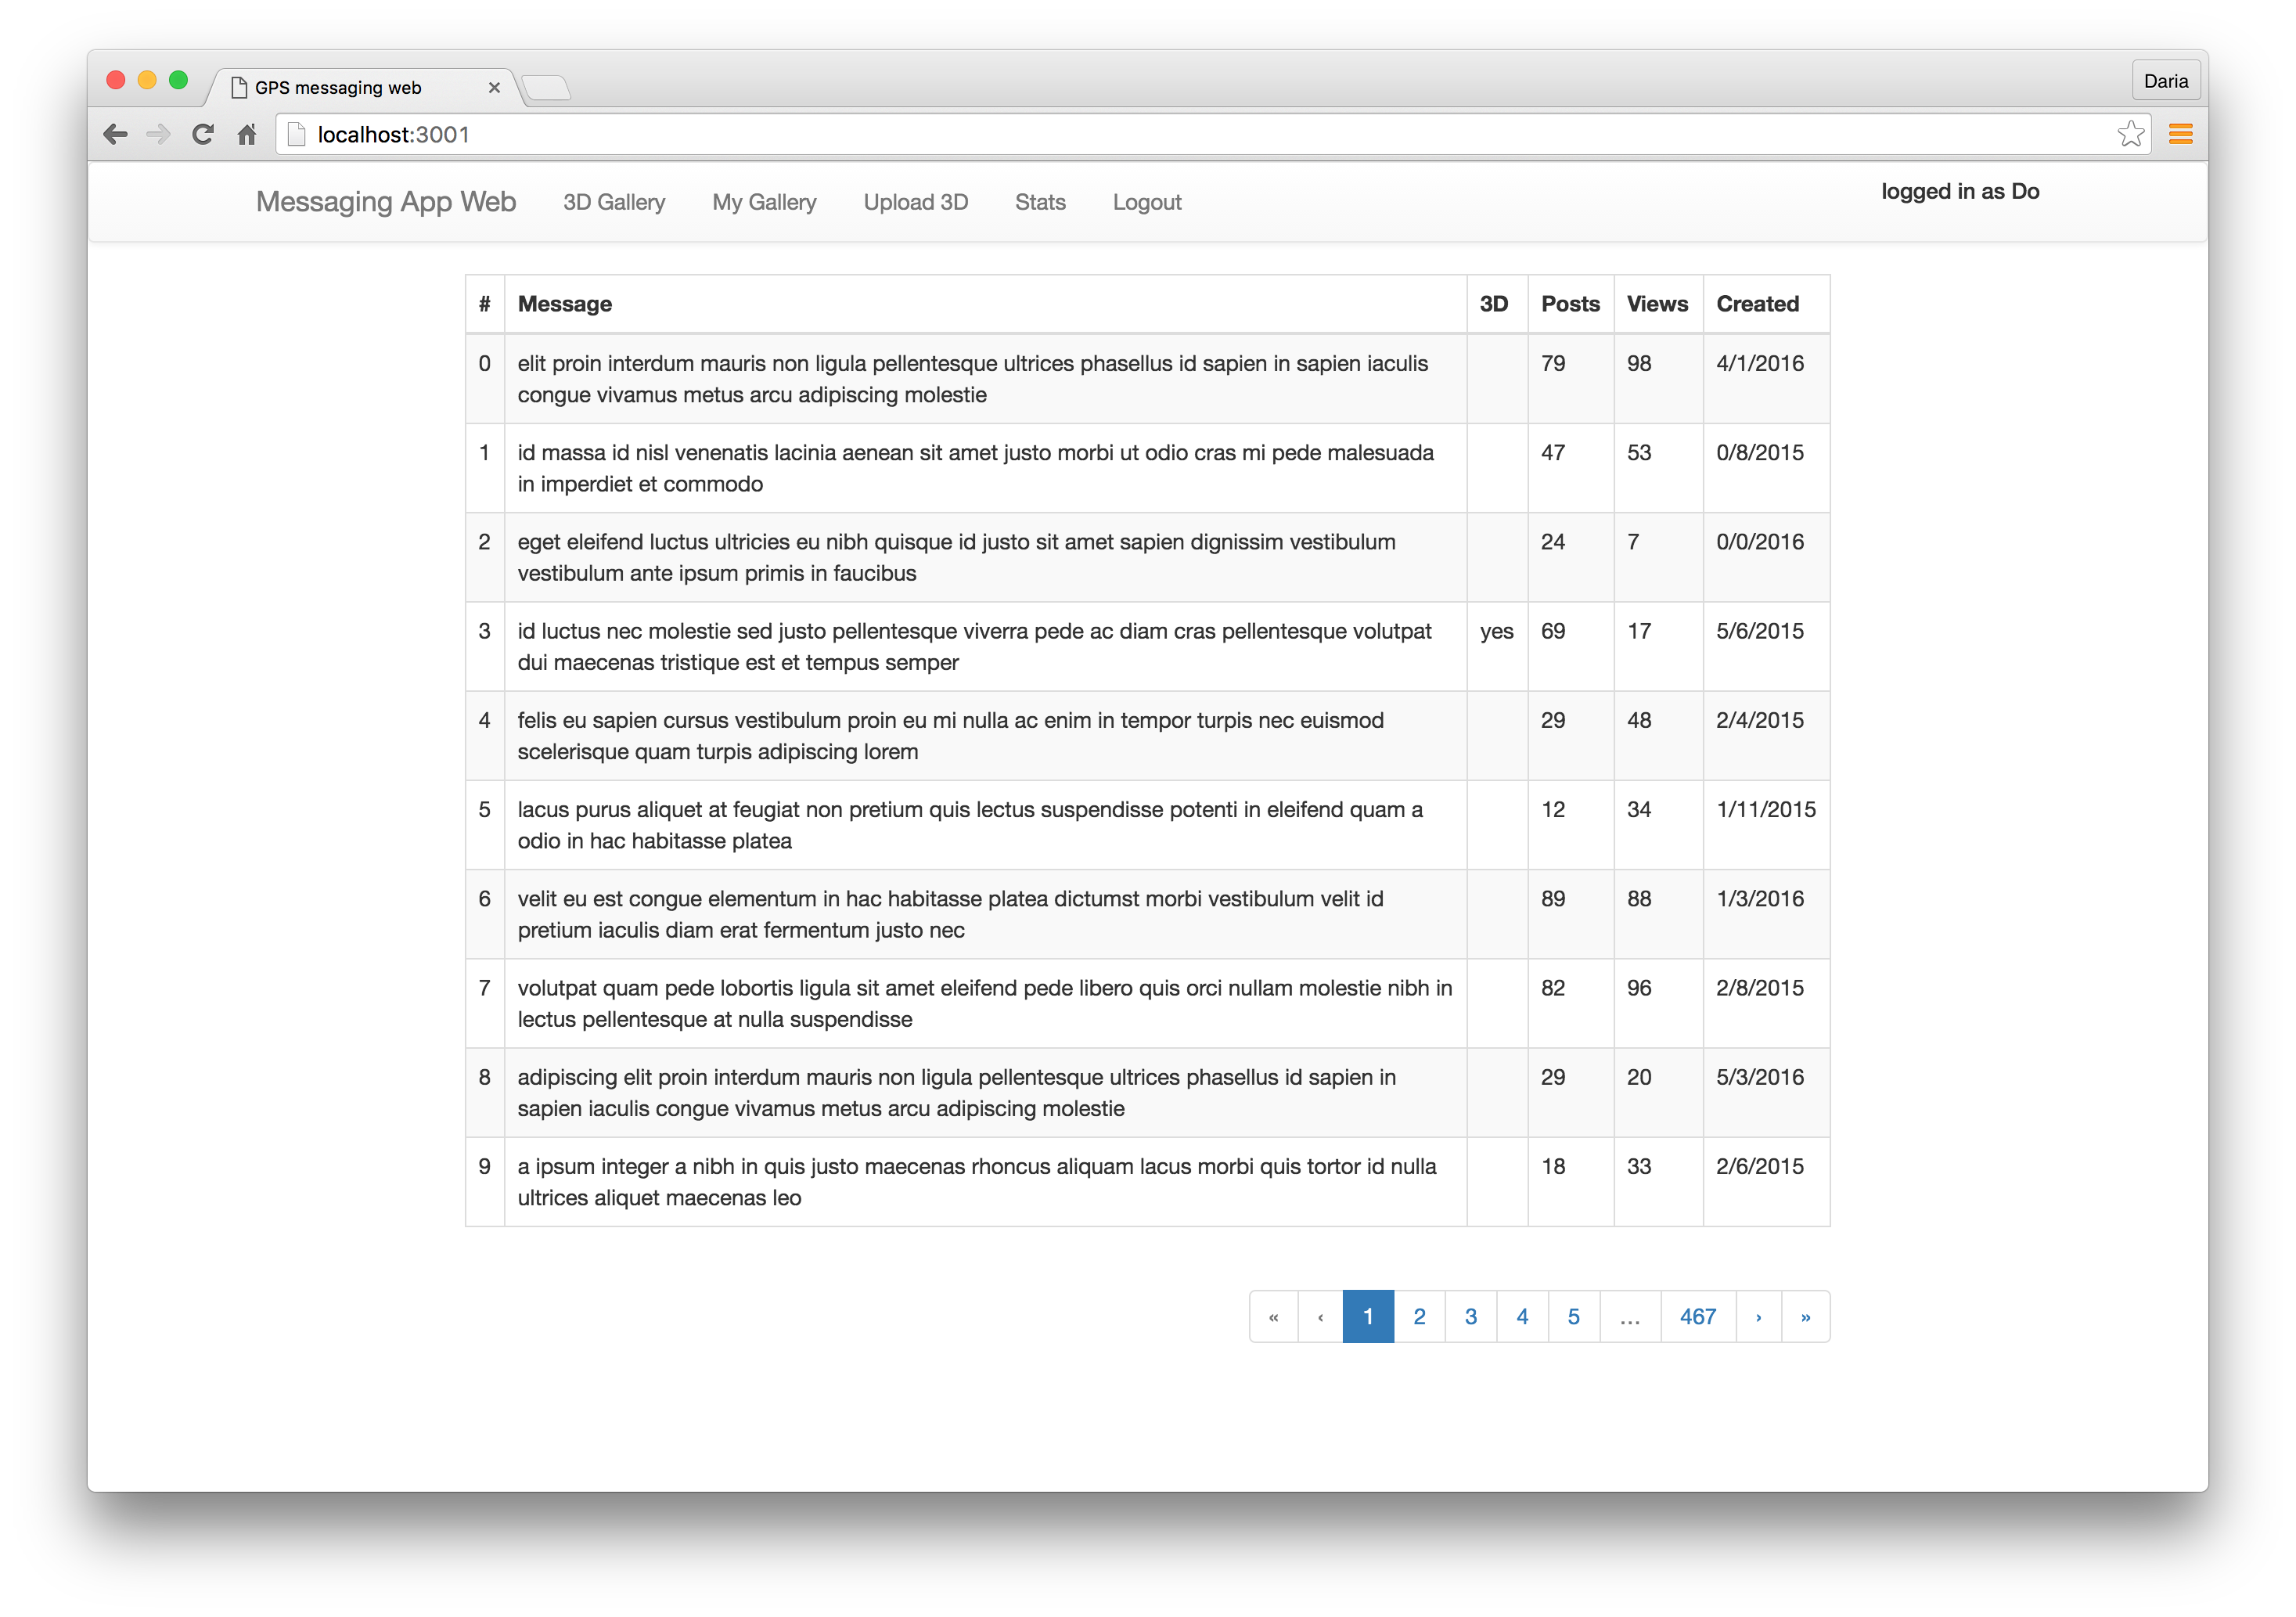
\includegraphics[width=0.8\textwidth]{assets/web_screens/index.png}}
	\caption{Web application. Index page with messages}
\end{figure}

\begin{figure}[!ht]
	\centering
	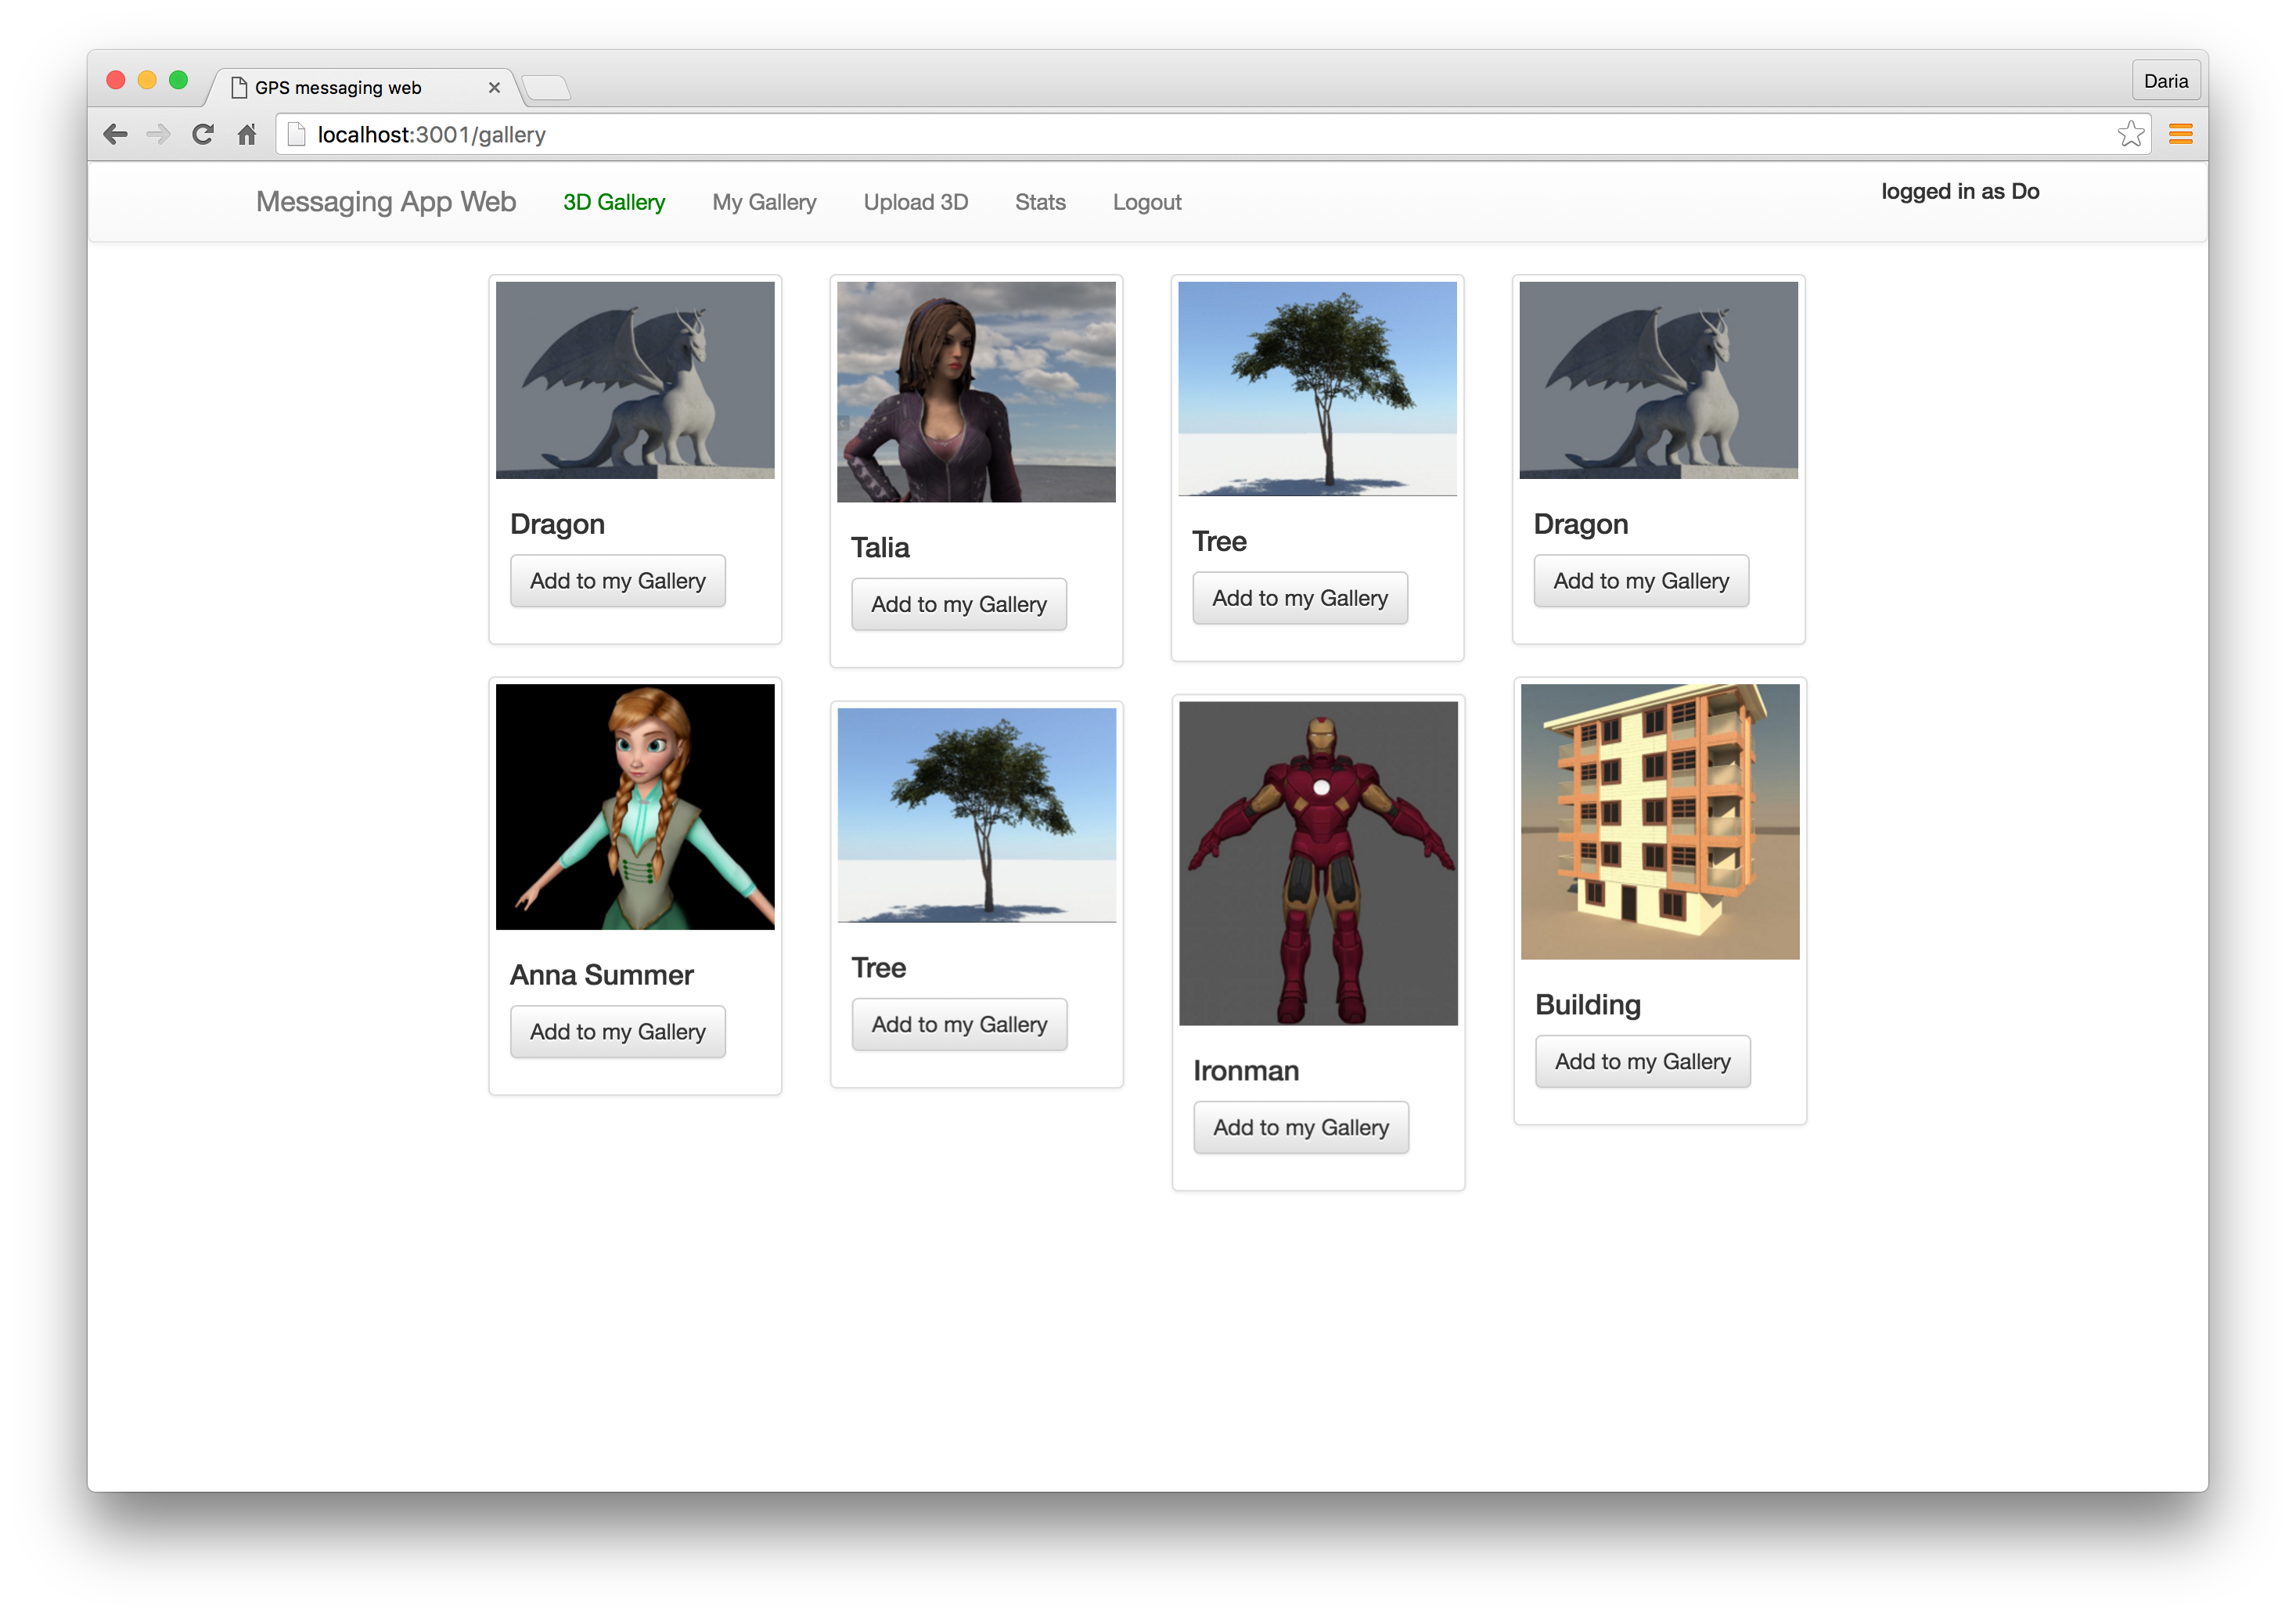
\includegraphics[width=0.8\textwidth]{assets/web_screens/3d_gallery.png}}
	\caption{Web application. 3D gallery with objects}
\end{figure}


\begin{figure}[!ht]
	\centering
	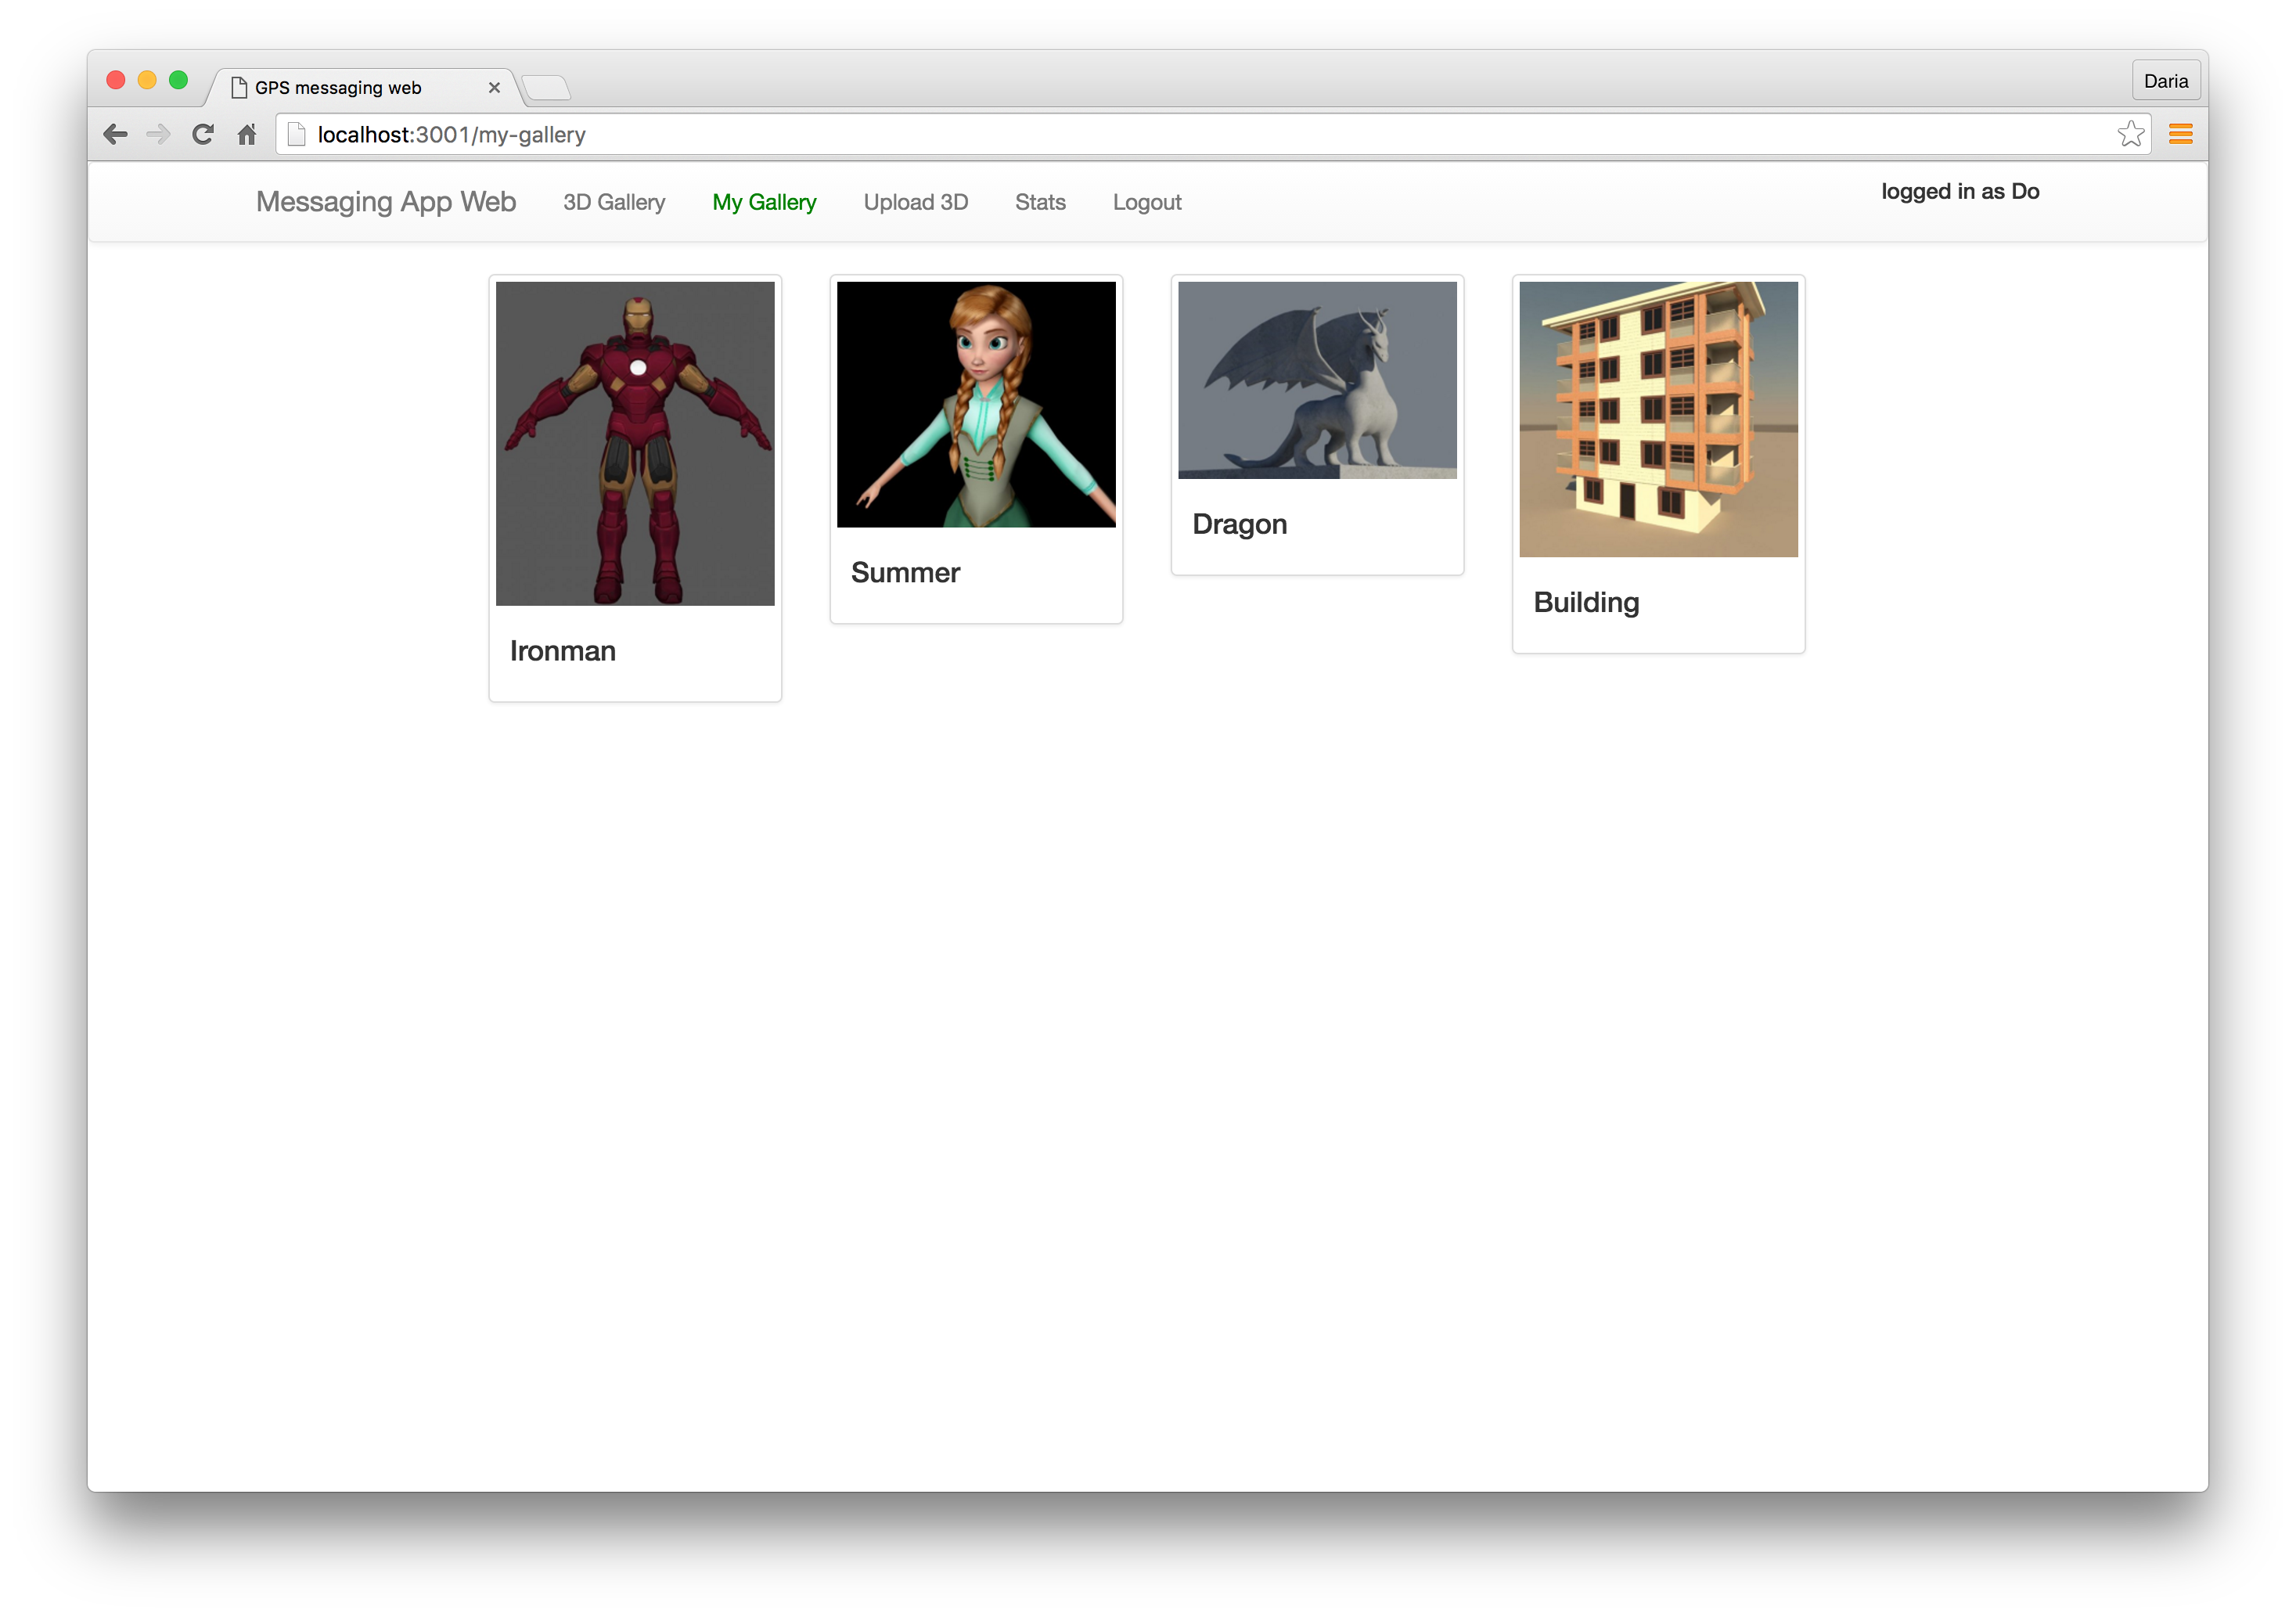
\includegraphics[width=0.8\textwidth]{assets/web_screens/my_gallery.png}}
	\caption{Web application. User's 3d gallery with objects}
\end{figure}


\begin{figure}[!ht]
	\centering
	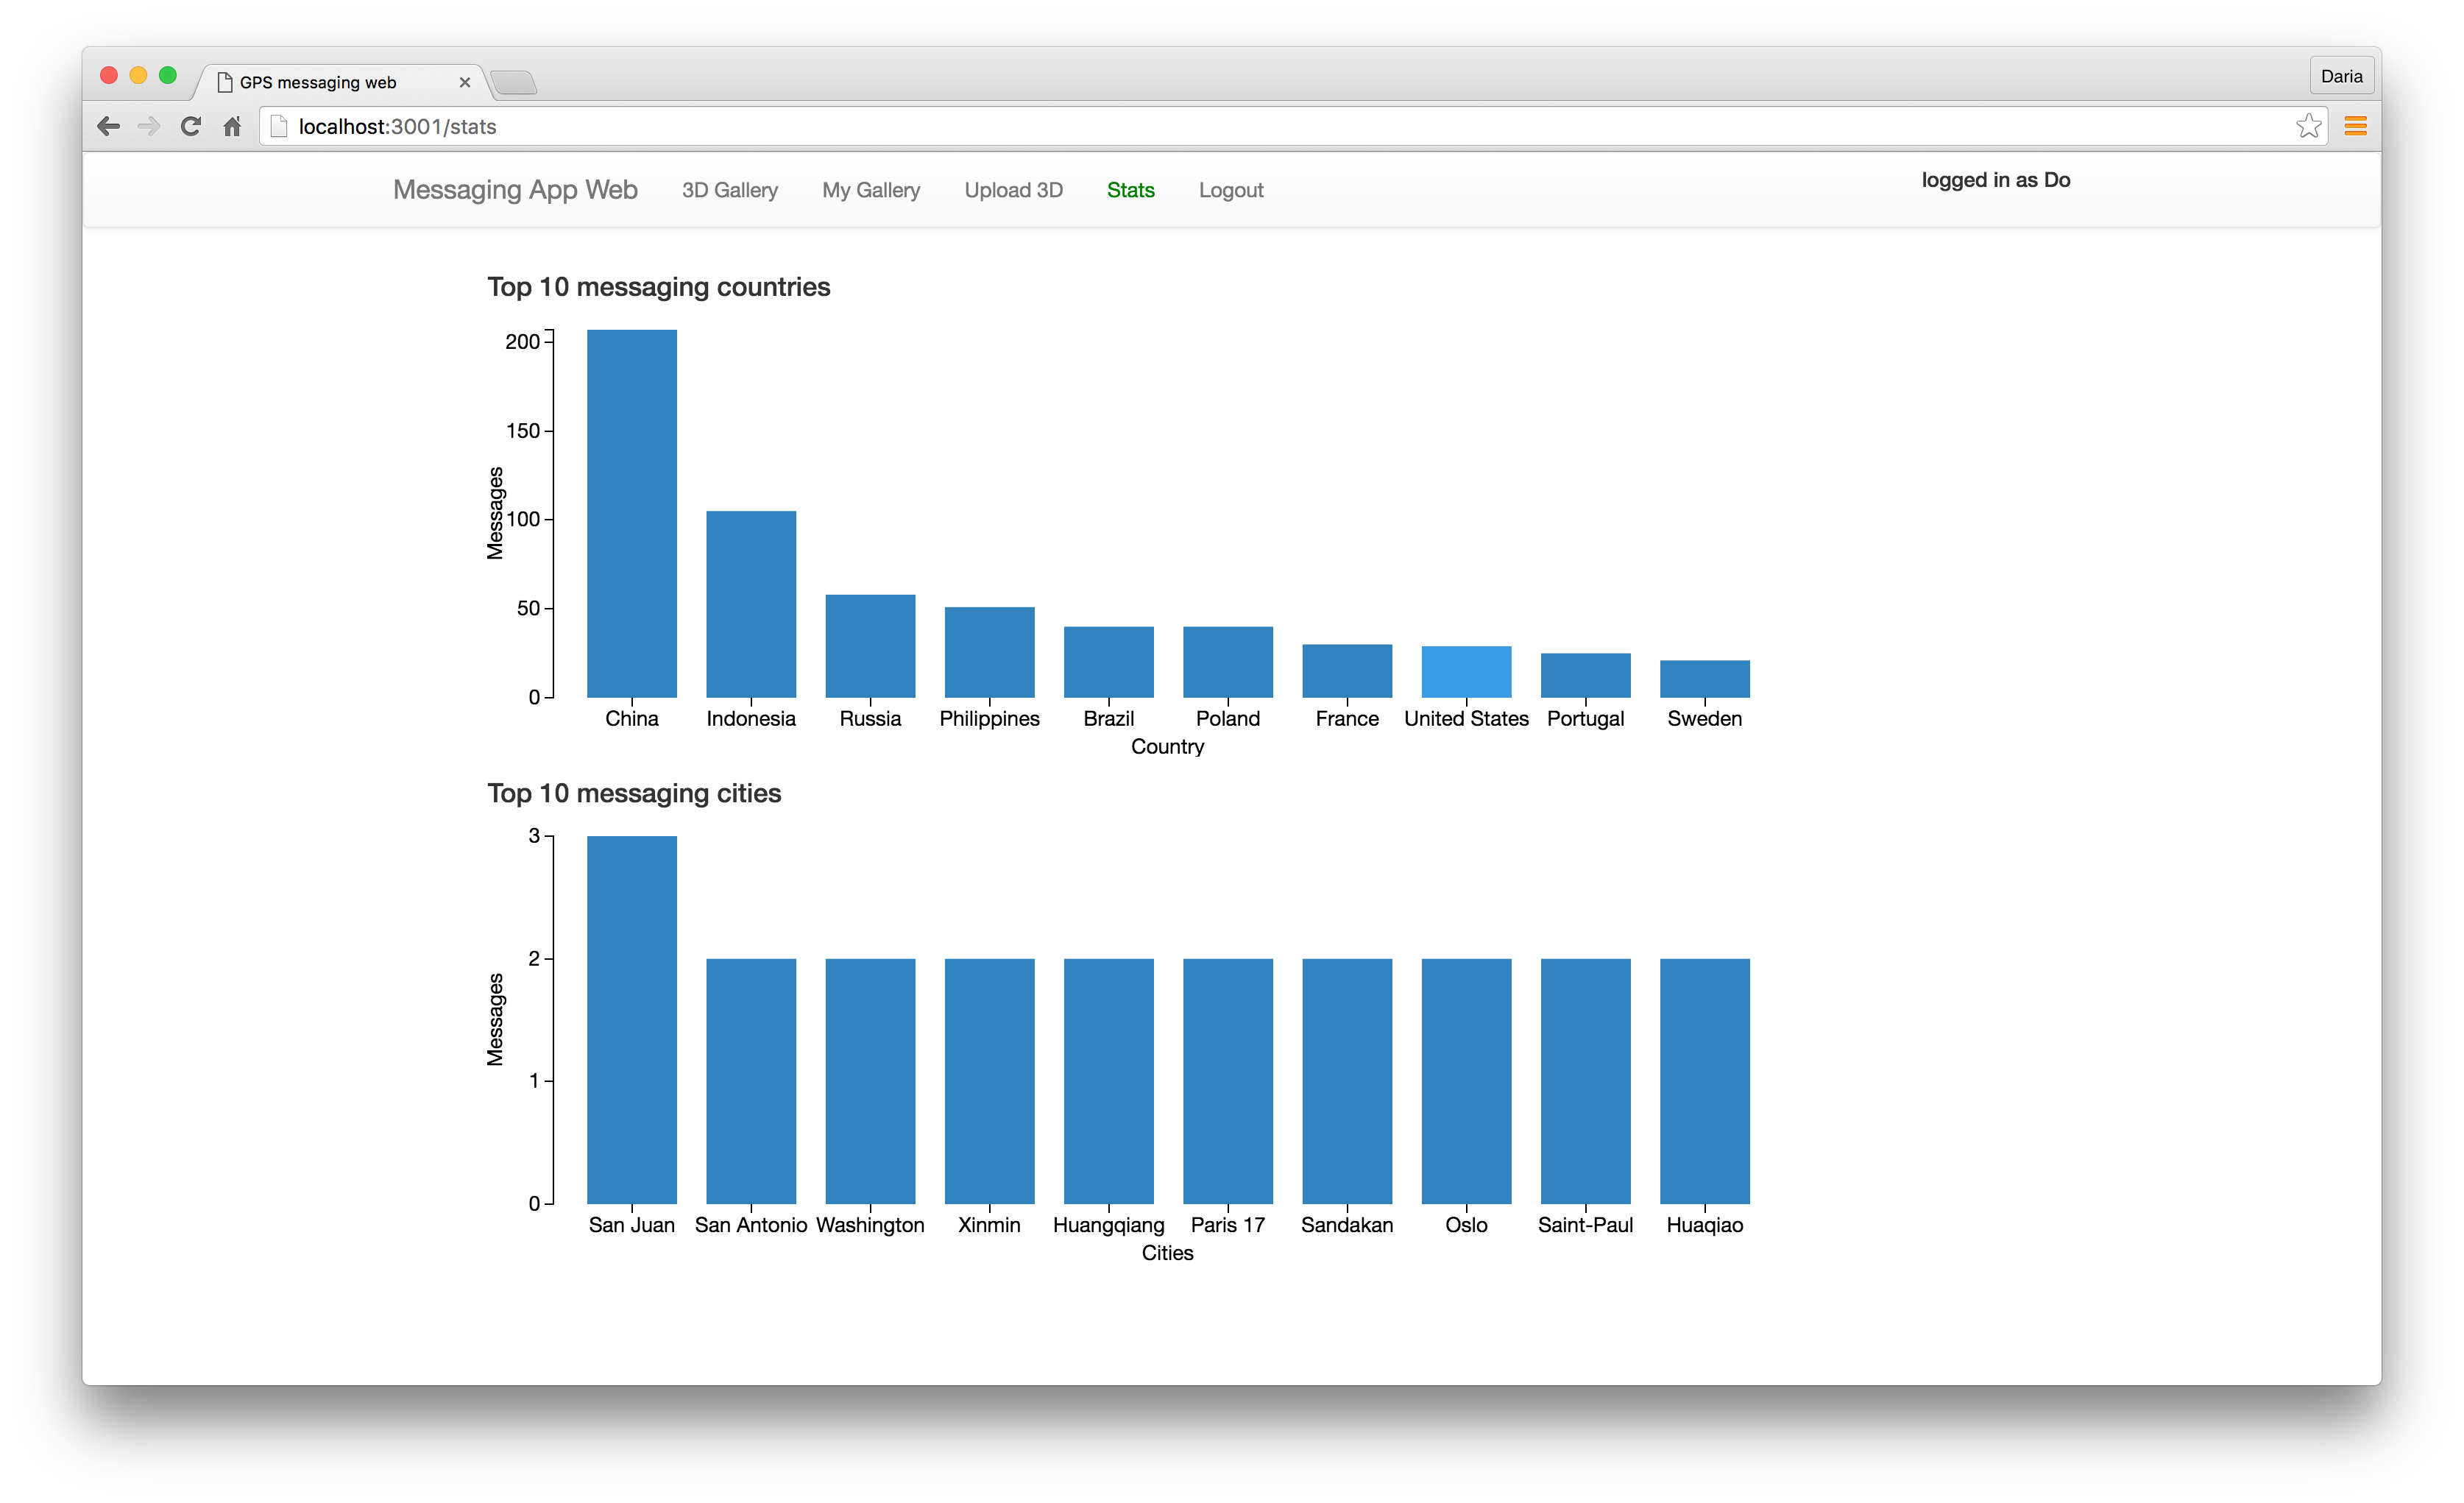
\includegraphics[width=0.8\textwidth]{assets/web_screens/stats.png}}
	\caption{Web application. Statistics}
\end{figure}

\chapter{Supervisor configuration}
\label{apx:supervisor}

Default directory for the supervisor is where the configuration file is. Most of the configuration is default, the only changed lines are 20 to 39, the program configuration.
\begin{lstlisting}[language=C]
[unix_http_server]
file=/tmp/supervisor.sock   ; (the path to the socket file)

[supervisord]
logfile=/supervisor/supervisord.log ; (main log file)
logfile_maxbytes=50MB        ; (max logfile bytes b4 rotation;)
logfile_backups=10           ; (main logfile rotation backups)
loglevel=info                ; (log level;default info;)
pidfile=/tmp/supervisord.pid ; (supervisord pidfile)
nodaemon=false               ; (start in foreground if true)
minfds=1024                  ; (min.  startup file descriptors)
minprocs=200                 ; (min.  process descriptors)

[rpcinterface:supervisor]
supervisor.rpcinterface_factory = supervisor.rpcinterface:make_main_rpcinterface

[supervisorctl]
serverurl=unix:///tmp/supervisor.sock ; use a unix:// URL  for a unix socket

[program:airServer]
command=npm start
autostart=true 
stdout_logfile=/logs/supervisor/server_out.log
stderr_logfile=/logs/supervisor/server_err.log  

[program:geoConsumer]
directory=/kue
command=node geoConsumer.js
autostart=true 
stdout_logfile=/logs/supervisor/geoConsumer_out.log
stderr_logfile=/logs/supervisor/geoConsumer_err.log  

[program:validConsumer]
directory=/kue
command=node validConsumer.js
autostart=true 
stdout_logfile=/logs/supervisor/validConsumer_out.log
stderr_logfile=/logs/supervisor/validConsumer_err.log  

\end{lstlisting}

\chapter{Express server for React routing}
\label{apx:react-server}

\begin{lstlisting}[language=JavaScript]
// required for converting JSX syntax
require("node-jsx").install();
require("babel-core/register")({"presets": ["es2015"]});
var express = require('express');
var path = require('path');
var app = express();

// serving static files
app.use(express.static(path.join(__dirname, 'public')));

app.get('*', function (request, response){
  response.sendFile(path.resolve(__dirname, 'public', 'index.html'))
});

// development error handler - will print stacktrace
if (app.get('env') === 'development') {
  app.use(function(err, req, res, next) {
    res.status(err.status || 500);
    res.render('error', {
      message: err.message,
      error: err
    });
  });
}

// production error handler - no stacktraces leaked to user
app.use(function(err, req, res, next) {
  res.status(err.status || 500);
  res.render('error', {
    message: err.message,
    error: {}
  });
});

module.exports = app;
\end{lstlisting}

\chapter{Integration of Wikitude and React Native}
\label{apendix:integration}
In order to integrate Wikitude and React Native I implemented the following files:
\begin{itemize}
\item \verb|ViewController.h| 
\item \verb|ViewController.m| - starting point for the Wikitude
\item \verb|ARViewManager.h|
\item \verb|ARViewManager.m| - exported view component for React Native
\end{itemize}

\begin{lstlisting}[language=C]
//  ViewController.h

#import <UIKit/UIKit.h>

@interface ViewController : UIViewController

@property (nonatomic, assign) NSString *objSrc;

@end

\end{lstlisting}

\begin{lstlisting}[language=C]
//  ViewController.m

#import "ViewController.h"

#import "View.h"
#import <WikitudeSDK/WikitudeSDK.h>
/* Wikitude SDK debugging */
#import <WikitudeSDK/WTArchitectViewDebugDelegate.h>

@interface ViewController () <WTArchitectViewDelegate, WTArchitectViewDebugDelegate>

/* Add a strong property to the main Wikitude SDK component, the WTArchitectView */
@property (nonatomic, strong) WTArchitectView               *architectView;

/* And keep a weak property to the navigation object which represents the loading status of your Architect World */
@property (nonatomic, weak) WTNavigation                    *architectWorldNavigation;

@end

@implementation ViewController


- (void)dealloc
{
  /* Remove this view controller from the default Notification Center so that it can be released properly */
  
  [[NSNotificationCenter defaultCenter] removeObserver:self];
}

- (void)loadView
{
  View *_view = [[View alloc] init];
  self.view = _view;
}


- (void)viewDidLoad {
  [super viewDidLoad];
  // Do any additional setup after loading the view, typically from a nib.
  
  /* It might be the case that the device which is running the application does not fulfil all Wikitude SDK hardware requirements.
   To check for this and handle the situation properly, use the -isDeviceSupportedForRequiredFeatures:error class method.
   
   Required features specify in more detail what your Architect World intends to do. Depending on your intentions, more or less devices might be supported.
   e.g. an iPod Touch is missing some hardware components so that Geo augmented reality does not work, but 2D tracking does.
   
   NOTE: On iOS, an unsupported device might be an iPhone 3GS for image recognition or an iPod Touch 4th generation for Geo augmented reality.
   */
  NSError *deviceSupportError = nil;

  if ( [WTArchitectView isDeviceSupportedForRequiredFeatures:WTFeature_Geo error:&deviceSupportError] ) {
    
    /* Standard WTArchitectView object creation and initial configuration */
    self.architectView = [[WTArchitectView alloc] initWithFrame:CGRectZero motionManager:nil];
    self.architectView.delegate = self;
    self.architectView.debugDelegate = self;
    
    /* Use the -setLicenseKey method to unlock all Wikitude SDK features that you bought with your license. */
    [self.architectView setLicenseKey:@"YOUR_KEY"];
    
    /* The Architect World can be loaded independently from the WTArchitectView rendering.
     
     NOTE: The architectWorldNavigation property is assigned at this point. The navigation object is valid until another Architect World is loaded.
     */
    
    NSURL *baseURL = [NSURL URLWithString:(@"http://192.168.0.3:3000/ArchitectWorld/index.html")];
    self.architectWorldNavigation = [self.architectView loadArchitectWorldFromURL:baseURL withRequiredFeatures:WTFeature_Geo];
    /* Because the WTArchitectView does some OpenGL rendering, frame updates have to be suspended and resumend when the application changes it's active state.
     Here, UIApplication notifications are used to respond to the active state changes.
     
     NOTE: Since the application will resign active even when an UIAlert is shown, some special handling is implemented in the UIApplicationDidBecomeActiveNotification.
     */
    [[NSNotificationCenter defaultCenter] addObserverForName:UIApplicationDidBecomeActiveNotification object:nil queue:[NSOperationQueue mainQueue] usingBlock:^(NSNotification *note) {
      
      /* When the application starts for the first time, several UIAlert's might be shown to ask the user for camera and/or GPS access.
       Because the WTArchitectView is paused when the application resigns active (See line 86), also Architect JavaScript evaluation is interrupted.
       To resume properly from the inactive state, the Architect World has to be reloaded if and only if an active Architect World load request was active at the time the application resigned active.
       This loading state/interruption can be detected using the navigation object that was returned from the -loadArchitectWorldFromURL:withRequiredFeatures method.
       */
      if (self.architectWorldNavigation.wasInterrupted) {
        [self.architectView reloadArchitectWorld];
      }
      
      /* Standard WTArchitectView rendering resuming after the application becomes active again */
      [self startWikitudeSDKRendering];
    }];
    [[NSNotificationCenter defaultCenter] addObserverForName:UIApplicationWillResignActiveNotification object:nil queue:[NSOperationQueue mainQueue] usingBlock:^(NSNotification *note) {
      
      /* Standard WTArchitectView rendering suspension when the application resignes active */
      [self stopWikitudeSDKRendering];
    }];
    
    /* Standard subview handling using Autolayout */
    [self.view addSubview:self.architectView];
    self.architectView.translatesAutoresizingMaskIntoConstraints = NO;
    
    NSDictionary *views = NSDictionaryOfVariableBindings(_architectView);
    [self.view addConstraints: [NSLayoutConstraint constraintsWithVisualFormat:@"|[_architectView]|" options:0 metrics:nil views:views] ];
    [self.view addConstraints: [NSLayoutConstraint constraintsWithVisualFormat:@"V:|[_architectView]|" options:0 metrics:nil views:views] ];
  }
  else {
    NSLog(@"This device is not supported. Show either an alert or use this class method even before presenting the view controller that manages the WTArchitectView. Error: %@", [deviceSupportError localizedDescription]);
  }
}

#pragma mark - View Lifecycle
- (void)viewWillAppear:(BOOL)animated {
  
  [super viewWillAppear:animated];
  View* test_view = [self view];
  NSString *src = [NSString stringWithFormat:@"%@%@%@%@%@", @"x(",@"\'" ,[test_view objSrc], @"\'", @");"];
  [self.architectView callJavaScript:(@"@a", src)];
  
  /* WTArchitectView rendering is started once the view controllers view will appear */
  [self startWikitudeSDKRendering];
}

- (void)viewDidDisappear:(BOOL)animated {
  [super viewDidDisappear:animated];
  
  /* WTArchitectView rendering is stopped once the view controllers view did disappear */
  [self stopWikitudeSDKRendering];
}

- (void)didReceiveMemoryWarning {
  [super didReceiveMemoryWarning];
  // Dispose of any resources that can be recreated.
}

#pragma mark - View Rotation
- (BOOL)shouldAutorotate {
  
  return YES;
}

- (NSUInteger)supportedInterfaceOrientations {
  
  return UIInterfaceOrientationMaskAll;
}

- (void)willRotateToInterfaceOrientation:(UIInterfaceOrientation)toInterfaceOrientation duration:(NSTimeInterval)duration {
  
  /* When the device orientation changes, specify if the WTArchitectView object should rotate as well */
  [self.architectView setShouldRotate:YES toInterfaceOrientation:toInterfaceOrientation];
}

#pragma mark - Private Methods

/* Convenience methods to manage WTArchitectView rendering. */
- (void)startWikitudeSDKRendering{
  
  /* To check if the WTArchitectView is currently rendering, the isRunning property can be used */
  if ( ![self.architectView isRunning] ) {
    /* To start WTArchitectView rendering and control the startup phase, the -start:completion method can be used */
    [self.architectView start:^(WTStartupConfiguration *configuration) {
      
      /* Use the configuration object to take control about the WTArchitectView startup phase */
      /* You can e.g. start with an active front camera instead of the default back camera */
      
//       configuration.captureDevicePosition = AVCaptureDevicePositionFront;
      
    } completion:^(BOOL isRunning, NSError *error) {
      
      /* The completion block is called right after the internal start method returns.
       
       NOTE: In case some requirements are not given, the WTArchitectView might not be started and returns NO for isRunning.
       To determine what caused the problem, the localized error description can be used.
       */
      if ( !isRunning ) {
        NSLog(@"WTArchitectView could not be started. Reason: %@", [error localizedDescription]);
      }
    }];
  }
}

- (void)stopWikitudeSDKRendering {
  
  /* The stop method is blocking until the rendering and camera access is stopped */
  if ( [self.architectView isRunning] ) {
    [self.architectView stop];
  }
}

/* The WTArchitectView provides two delegates to interact with. */
#pragma mark - Delegation

/* The standard delegate can be used to get information about:
 * The Architect World loading progress
 * architectsdk:// protocol invocations using document.location inside JavaScript
 * Managing view capturing
 * Customizing view controller presentation that is triggered from the WTArchitectView
 */
#pragma mark WTArchitectViewDelegate
- (void)architectView:(WTArchitectView *)architectView didFinishLoadArchitectWorldNavigation:(WTNavigation *)navigation {
  /* Architect World did finish loading */
}

- (void)architectView:(WTArchitectView *)architectView didFailToLoadArchitectWorldNavigation:(WTNavigation *)navigation withError:(NSError *)error {
  
  NSLog(@"Architect World from URL '%@' could not be loaded. Reason: %@", navigation.originalURL, [error localizedDescription]);
}

/* The debug delegate can be used to respond to internal issues, e.g. the user declined camera or GPS access.
 
 NOTE: The debug delegate method -architectView:didEncounterInternalWarning is currently not used.
 */
#pragma mark WTArchitectViewDebugDelegate
- (void)architectView:(WTArchitectView *)architectView didEncounterInternalWarning:(WTWarning *)warning {
  
  /* Intentionally Left Blank */
}

- (void)architectView:(WTArchitectView *)architectView didEncounterInternalError:(NSError *)error {
  
  NSLog(@"WTArchitectView encountered an internal error '%@'", [error localizedDescription]);
}


@end
\end{lstlisting}

\clearpage
\begin{lstlisting}[language=C]
//  ARViewManager.h

#import "RCTViewManager.h"

@interface ARViewManager : RCTViewManager

@end

\end{lstlisting}

\begin{lstlisting}[language=C]
//  ARViewManager.m

#import "ARViewManager.h"
#import "ViewController.h"
#import "View.h"

@implementation ARViewManager

RCT_EXPORT_MODULE()

RCT_EXPORT_VIEW_PROPERTY(objSrc, NSString);

- (UIView *)view
{
  ViewController *_controller = [[ViewController alloc] init];
  return _controller.view;
}

@end
\end{lstlisting}

\chapter{Contents of enclosed CD}

%change appropriately

\begin{figure}
	\dirtree{%
		.1 readme.txt\DTcomment{the file with CD contents description}.
		.1 exe\DTcomment{the directory with executables}.
		.1 src\DTcomment{the directory of source codes}.
		.2 wbdcm\DTcomment{implementation sources}.
		.2 thesis\DTcomment{the directory of \LaTeX{} source codes of the thesis}.
		.1 text\DTcomment{the thesis text directory}.
		.2 thesis.pdf\DTcomment{the thesis text in PDF format}.
		.2 thesis.ps\DTcomment{the thesis text in PS format}.
	}
\end{figure}

\end{document}
